% IEEE Paper Template for US-LETTER Page Size (V1)
% Sample Conference Paper using IEEE LaTeX style file for US-LETTER pagesize.
% Copyright (C) 2006-2008 Causal Productions Pty Ltd.
% Permission is granted to distribute and revise this file provided that
% this header remains intact.
%
% REVISION HISTORY
% 20080211 changed some space characters in the title-author block
%
\documentclass[10pt,conference,letterpaper]{IEEEtran}
\usepackage{times,amsmath,epsfig}
\usepackage{algorithm}
\usepackage{algorithmic}
\usepackage{epstopdf}
\usepackage{graphicx}
\renewcommand{\algorithmicrequire}{\textbf{Input:}} 
\renewcommand{\algorithmicensure}{\textbf{Output:}}
\usepackage[tight,footnotesize]{subfigure}
\usepackage{amsfonts}
\usepackage{xspace}
\newcommand{\tabincell}[2]{\begin{tabular}{@{}#1@{}}#2\end{tabular}}  
\newcommand{\frname}{GAT\xspace }
\newcommand{\idxname}{GTIDX\xspace }
\newcommand{\rangeq}{{{\cal Q}_r}\xspace}
\newcommand{\simq}{{{\cal Q}_k}\xspace}
\newcommand{\rangecand}{{{\cal Q}_r^c}\xspace}
\newcommand{\simcand}{{{\cal Q}_k^c}\xspace}
\newcommand{\alltraj}{{{\cal T}}\xspace}
\newcommand{\edr}{{\delta}\xspace}
\newcommand{\allcell}{{\cal C}\xspace}
\newcommand{\trajcell}{{f_c}\xspace}
\newcommand{\trajtable}{{\cal S}\xspace}
\newcommand{\quadtree}{{\cal P}\xspace}
\newcommand{\rangecandnode}{{{\cal C}_r^c}\xspace}
\newcommand{\eat}[1]{}
\newtheorem{definition}{Definition}
\newtheorem{theorem}{Theorem}

%
\title{An Efficient GPU-accelerated Framework for Answering Trajectory Queries}
%
\author{%
% author names are typeset in 11pt, which is the default size in the author block
{Bowen Zhang{\small $~$}, Yanmin Zhu{\small $~$}, Yanyan Shen{\small $~$} }%
% add some space between author names and affils
\vspace{1.6mm}\\
\fontsize{10}{10}\selectfont\itshape
% 20080211 CAUSAL PRODUCTIONS
% separate superscript on following line from affiliation using narrow space
$^{\#}$\,Department of Computer Science and Engeneering, Shanghai Jiao Tong University\\
Shanghai, China 200240\\
\fontsize{9}{9}\selectfont\ttfamily\upshape
%
% 20080211 CAUSAL PRODUCTIONS
% in the following email addresses, separate the superscript from the email address 
% using a narrow space \,
% the reason is that Acrobat Reader has an option to auto-detect urls and email
% addresses, and make them 'hot'.  Without a narrow space, the superscript is included
% in the email address and corrupts it.
% Also, removed ~ from pre-superscript since it does not seem to serve any purpose
\{zbw0046,yzhu,shenyy\}@sjtu.edu.cn\\
% add some space between email and affil
\vspace{1.2mm}\\
\fontsize{10}{10}\selectfont\rmfamily\itshape
% 20080211 CAUSAL PRODUCTIONS
% separated superscript on following line from affiliation using narrow space \,
%$^{*}$\,Second Company\\
%Address Including Country Name\\
%\fontsize{9}{9}\selectfont\ttfamily\upshape
%% 20080211 CAUSAL PRODUCTIONS
%% removed ~ from pre-superscript since it does not seem to serve any purpose
%$^{2}$\,second.author@second.com
}
%
\begin{document}
\maketitle
%
\begin{abstract} 
As the development of smart devices equipped with GPS, here comes a large amount of trajectory data, implying many useful information about our daily life. This calls for a trajectory analytics framework able to process mass of various kinds of queries efficiently. GPU, which has been widely equipped in data centers, can accelerate queries by handling them in parallel. However, existing GPU-accelerated trajectory storage systems are optimized for specific kind of query, suffering from the problem of efficiency when they are used for processing queries they are not optimized for. To solve this problem, we propose a framework optimized for the features of GPU which supports both two basic kinds of queries for big trajectory data. We design a unified storage component with an index called \idxname with a cell-based trajectory storage, which combines and links quadtree, grid and trajectories together to support pruning methods for two basic kinds of queries. Based on the storage component, to make full use of the parallel power of GPU, the query processing in our framework is optimized for the issues of GPU computing including load-balancing, coalesce memory accessing and less data transferring. We implement our framework and evaluate it on two real-life trajectory datasets, which shows our framework is able to conduct two basic types of queries on large scale trajectory data efficiently. Moreover, our framework achieves a speedup of 38x for range query and 67x for top-k similarity query than the implementation on CPU, demonstrating that our framework really achieves the goal of accelerating both two kinds of queries on large-scale trajectory data by GPU.
\end{abstract}

% NOTE keywords are not used for conference papers so do not populate them
% \begin{keywords}
% keyword-1, keyword-2, keyword-3
% \end{keywords}
%

\section{Introduction}
% no \IEEEPARstart

%What is the problem?
%Why is it interesting and important?

%the emergence of large volumes of trajectory data
%Two kinds of trajectory queries, range query and knn query, are essential operations in various applications..
%the objectives of trajectory query processing: (i) effciency; (ii) high throughput; (iii) others?? 

With the rapid development of wireless communication and mobile computing techniques, large amounts of spatial trajectories have been generated continuously from every corner of the world.
%shenyy:real-life statistics?
%zbw:add an example about DIDI
For example, a Chinese online transportation network company called DiDi is processing over 3 million trips every day in China~\cite{DidiExample}, and millions of trajectories produced by these trips are recorded in real time to improve the quality of service.
A \emph{trajectory} is typically represented as a sequence of successive points of moving objects, where each point consists of geospatial coordinates and a timestamp. 
The emergence of such trajectory data facilitates a wide spectrum of applications including route planing~\cite{RoutePlan}, trajectory pattern mining~\cite{DBLP:journals/tkde/ZhengZYSZ14} and travel time prediction~\cite{DBLP:conf/gis/LeeSCC12}.
%
In all these applications, two kinds of trajectory queries, \emph{range query} and \emph{similarity query}, serve as primitive, yet essential operations.

%Developing a unified framework tailored for answering two kinds of trajectory queries is challenging.
Range queries aim to identify trajectories overlapped with a given bounding area, while similarity queries determine $k$ trajectories that are closest to the query trajectory measured by a distance function. 
In some tasks, two kinds of queries are performed in a collaborative manner. For example, when planing driving routes, a backend system first needs to predict travel time by estimating real-time vehicle densities in all the relevant areas using range queries and then submits a top-$k$ similarity query to search for historical trajectories that require similar travel time to get the final results.

However, developing a unified framework tailored for answering both range and similarity trajectory queries is challenging. 
On the one hand, both queries are expansive to compute, in face of mountains (e.g., hundreds of millions) of candidate trajectories. Specifically, it is infeasible to perform sequential scan over all trajectory data to produce results.
On the other hand, in reality, it is very likely that a batch of trajectory queries are issued in a short time period that require parallel processing.
Examples include estimating trajectory density in different areas, extracting moving patterns using clustering methods, answering queries from concurrent users in location-based services, and so on.

%Why is it hard? (E.g., why do naive approaches fail?)
%why it fails? analysis.

%general query processing systems -- inefficiency
%specialized trajectory query processing systems -- examples (single-machine, distributed system, GPU-acclerated), limitations -- (i) (single machine): performance is bounded by CPU cores; low throughput, eg; (ii) problems of distributed solutions???

While traditional databases or data processing frameworks (e.g., SparkSQL~\cite{DBLP:conf/sigmod/ArmbrustXLHLBMK15}) provide generic and high-throughput solutions to coping with two kinds of trajectory queries, the performance is always suboptimal, probably due to the lack of delicately designed index for querying trajectories. 
Recently, considerable research efforts have been devoted to developing specialized trajectory query processing systems (e.g., Simba~\cite{DBLP:conf/sigmod/XieL0LZG16}, SharkDB~\cite{DBLP:conf/cikm/WangZXZZS14}).
%
However, these state-of-the-art solutions are typically designed for answering either range or similarity queries, but not both. To handle both trajectory queries, they rely on separate indices with different parameter settings, which may introduce problems such as data duplication and index inconsistency. Furthermore, the performance of these systems can be limited by the computational power of CPU cores and suffer from low throughput for processing queries in batch. It was reported in Sayan's work~\cite{EDWP15} that
the total execution time of 10 top-5 similarity queries exceeds 700 seconds.
%%shenyy: the result is based on what kind of method??



%using GPU to acclerate performance, why -- (i) recent success of GPU-based query processing systems; (ii)highly parallel and high thoughput, other reasons?
%problems with GPU-solutions: (i) optimized for one particular query; (ii) simple similarity function; (iii) seldomly consider a batch of incoming queries, not optimize througput
To scale up the performance, a natural solution is to exploit GPU to accelerate query processing. GPU has been widely applied in high performance computing areas, thanks to its large amounts of parallelism~\cite{DBLP:journals/pvldb/ZhangWYGLZ15,7498315,DBLP:conf/icde/ChenDS17,DBLP:conf/bigdataconf/LealGZY15}.
To our best knowledge, however, only one recent work~\cite{GPUTaxi} attempted at leveraging GPUs to accelerate trajectory query processing. They proposed a grid-based index for PIP-test and processed similarity trajectory queries using the Hausdorff distance function~\cite{munkres2000topology}. 
In spite of its simple calculation, Hausdorff distance is not robust to handle trajectories with local time shifting, which is a common phenomenon in almost all trajectories~\cite{EDWP15}.
Moreover, the framework cannot be applied to answering range queries efficiently.
%Consequently, various distance metrics have been proposed to retrieve similar trajectories in the presence of noise and local time shifting.


%What are the key components of my approach and results? Also include any specific limitations.

%In this paper, we propose an in-memory GPU-acclerate .. framework for answering two trajectory queries efficiently. 
%Objectives: 
%key components: (i) follow filtering-verification framework based on CPU-GPU architecture. At a high level, ...; (ii) cell-based trajectory representation + a unified indexing, GT-quadtree?? (iii) use XXX similarty function for similarity queries; 

%Challenging issues: (i) data transfer cost between main memory and GPU memory due to high latency of PCI interfaces; (ii) load balance among thousands of GPU cores.
%our solutions: 
%key results:



In this paper, we develop an efficient GPU-accelerated framework, named \frname, for answering range and similarity trajectory queries in a unified way. We adopt the EDR~\cite{DBLP:conf/sigmod/ChenOO05} as the distance function for top-$k$ similarity queries, which is widely used to achieve global alignment. At a high level, \frname follows the filter-and-refine framework where CPU is responsible for generating candidate trajectories via effective pruning rules and GPU performs parallel candidate verification to get the final results.
%The filtering basis of \frname is a novel \idxname index that subtly fuses the merits of PR-quadtree~\cite{DBLP:conf/gis/LettichOS15} and cell-level trajectory representations, to reduce the number of candidate trajectories.
The filtering basis of \frname is a novel \idxname index that subtly fuses the merits of a fixed grid, PR-quadtree~\cite{DBLP:conf/gis/LettichOS15} and cell-level trajectory representations, to reduce the number of candidates in the process of two kinds of queries.
%
During verification, for range queries, we leverage GPUs to determine whether each candidate trajectory is overlapped with a given bounding area in parallel; for top-$k$ similarity queries, we iteratively supply GPUs with a set of candidate trajectories, parallelize each EDR distance computation, and progressively refine a priority queue that maintains possible top-$k$ answers based on the verification results. 

%zbw:add challenge (iii) data placement and operation obeying coalesce access pattern
In terms of the implementation, we address several practical issues to further accelerate trajectory query processing. One challenging issue is the low latency for transferring data between main memory and the global memory in GPU via PCIe interface. In addition to the index, we build a Memory Allocated Table (MAT) to check the existence of candidate trajectories and avoid redundant data transfer effectively. 
High latency of global memory in GPU is also a considerable challenge. In range query processing, we apply the Morton-based encoding method~\cite{DBLP:conf/gis/LettichOS15} to reorganize trajectory data; In similarity query, we place the state data produced in EDR calculation according to the order of CUDA threads. By these designs the data requested by a GPU Streaming Multiprocessor (SM) reside in continuous memory space and the retrieval requests over such continuous data can be coalesced to a large extent, so the number of high-latency memory transactions can be reduced and the throughput is improved.
Another issue is to achieve load balance among GPU cores. We address this problem by grouping fine-grained cells into blocks with similar number of trajectories points, which guarantees the computation workload balance among different GPU SMs. 

The main contributions of this work is the following.
\begin{itemize}
	\item We develop an efficient GPU-accelerated framework named \frname to support both range and top-$k$ similarity queries. \frname follows the generic filter-and-refine framework, where we use CPU to compute candidate trajectories and leverage GPU to conduct parallel verifications to increase throughput.
	\item We design a \idxname index over large-scale trajectory data, which is effective in pruning invalid candidates for both kinds of trajectory queries.
	\item We incorporate two kinds of optimizations into \frname: 
	We propose an algorithm of accelerating the calculation of EDR based on the \idxname index on GPU.
	\item We conduct extensive experiments to evaluate the performance of \frname using real datasets. The results show that 
	our system on two real-life datasets and evaluate its performance, proving that it gets about 38x speedup for range query and 67x speedup for top-k similarity query respectively comparing to the implementation on single-core CPU with an acceptable memory occupation.
\end{itemize}

The remainder of this paper is organized as follows. Section~\ref{sec:prelim} provides definitions and background. 
After that, in Section~\ref{sec:archi} we briefly introduce the architecture of our framework. We propose our design of storage component in Section~\ref{sec:index}. The query processing component is described in detail in Section~\ref{sec:query}. Some optimization on implementation level is introduced in Section~\ref{sec:optimization}. In Section~\ref{sec:exp}, we evaluate our system and results are reported. Some related works are summarized in Section~\ref{sec:related}, while Section~\ref{sec:conclusion} concludes the paper. 


\eat{
\section{Introduction}
% no \IEEEPARstart

As the number of mobile location devices (e.g., smartphones, cars, public bicycles, etc.) grows, increasing amount of spatial-temporal sequential data called trajectories are collected from the every corner of the world. For example, some map-based services such as Uber, Didi and BaiduMap record the location of millions of users in real time to improve the quality of service. There are a large amount of interesting and valuable information inside these data to be exploited, such as the moving pattern of citizens and the hotspot location in a city. A series of interesting applications are based on big trajectory data, such as route planing~\cite{RoutePlan}, trajectory pattern mining~\cite{DBLP:journals/tkde/ZhengZYSZ14}, travel time prediction~\cite{DBLP:conf/gis/LeeSCC12} and so on. 

What plays an important role in the applications is trajectory query processing.  For example, in travel time prediction, the range query is needed to estimate the density of the cars of a given area, and a top-k similarity query is executed to search for a trajectory which is more likely to have a similar travel time. As the development of mobile Internet, thousands of queries are produced every second in these applications because of the sharply increasing users. This situation calls for a solution of trajectory analytical framework with high throughput over large-scale trajectory data. 

Most traditional databases and big data processing frameworks (e.g., MySQL, SparkSQL~\cite{DBLP:conf/sigmod/ArmbrustXLHLBMK15}) designed for structured data can be used to process queries on large-scale trajectory data. However, they usually show poor performance because of no specific index for trajecory. For example, to finish a range query, two sets need to be produced by scaning whole dataset on each dimension and then an intersection need to be performed, which are extremely time-consuming.

Recent years various kinds of indices and in-memory storage such as Simba~\cite{DBLP:conf/sigmod/XieL0LZG16} and SharkDB~\cite{DBLP:conf/cikm/WangZXZZS14} are proposed to increase throughput of spatial queries for trajectories. Most of them are designed for specific kind of query, e.g. range query or top-k similarity query. However, in many applications such as travel time prediction mentioned above, both range query and top-k similarity query are both required. In this situation, these approaches fail in the efficiency of executing queries which they are not optimized for. On the other hand, the performance of these approaches is limited by the computational power of CPU. For example, it is reported in Sayan's work~\cite{EDWP15} that the execution time of 10 top-5 similarity query is about 700 seconds, whose throughput is quite low. 

% Although multithread and multicore CPU technology mitigate this problem to some extent, but the speedup is limited to the number of cores on the CPU chip.

As a manycore processor, GPU can achieve high throughput by executing tasks on thousands of cores at a time. For example, Mega-KV\cite{DBLP:journals/pvldb/ZhangWYGLZ15} gets 2.8x higher throughput than state-of-the-art approach of hash table performance in KV-store by the acceleration of GPU. Having witnessed that GPU has been widely applied in some works~\cite{7498315}~\cite{DBLP:conf/icde/ChenDS17}~\cite{DBLP:conf/bigdataconf/LealGZY15}, it is an excellent idea to accelerate a large number of queries on big trajectory data by leveraging strong ability of parallel computing of GPU.

However, as far as we know, only Zhang et.al. proposed a grid-based index~\cite{GPUTaxi} and then developed several algorithms about PIP-test~\cite{DBLP:journals/is/ZhangYG14} and similarity query~\cite{DBLP:conf/bigdata/LealGZY16} which leveraging GPU to accelerate the query processing of trajectories. Moreover, the similarity metric called Hausdorff distance~\cite{munkres2000topology} used in this work is too simple to handle trajectories with local time shifting, which is a common phenomenon because of different speed and sample rate of sensors on cars\cite{EDWP15}. In these years various robust similarity metrics which are based on global alignment are proposed to handle local time shifting, such as \textit{Edit Distance on Real Sequence} (EDR)~\cite{DBLP:conf/sigmod/ChenOO05}, \textit{Longest Common Sub-Sequence} (LCSS)~\cite{DBLP:conf/icde/VlachosGK02}, \textit{Dynamic Time Warping} (DTW)~\cite{DBLP:conf/vldb/Keogh02} and \textit{Edit Distance with Projections} (EDwP)~\cite{EDWP15}. However, the computations of them are expensive because of the high complexity algorithm. It is highly valuable for trajectory analytics frameworks to accelerate these computations and reduce the time cost by some parallel computing devices such as GPU. 

%However, the performance of large-scale trajectory query processing is still limited by the single-core CPU, which can only handle queries serially. For example, it is reported in ~\cite{EDWP15} that the execution time of a top-5 similarity query is about x seconds, which is quite slow for some interactive applications. Although multithread and multicore CPU technology mitigate this problem to some extent, but the speedup is limited to the number of cores on the CPU chip. Having witnessed the growing application of GPU in large-scale data processing, it is a popular choice that use it to answer mass of queries in parallel~\cite{7498315}[...]. As a many-core architecture processor, GPU can achieve high throughtput by running thousands of threads at a time.

%However, it is not trivial to accelerate all query processing by using GPU. Although a mass of query algorithm are designed for different purposes recently, they can be concluded in two main types: range-based query and trajectory-based query, which can be represented by two basic type of spatial queries: range query and top-k trajectory similarity query respectively.~\cite{DBLP:journals/tist/Zheng15} This two kinds of query are both indispensable for many kinds of trajectory applications. For example, they are both invoked in the process of travel time prediction~\cite{DBLP:conf/gis/LeeSCC12}. In this situation, query delay is significantly important for user's experience. So, it is valuable to develope a trajectory storage system which can make use of GPU to efficiently execute those different kinds of queries in a short response time. However, existing GPU-accelerated trajectory storage systems are almost optimized for specific kind of query, causing that applications invoking different kinds of query lose efficiency when running on them. Also, the index designed for CPU can not be easily migrated to GPU because of the significantly different architecture. It is not wise to trivially add an additional query module to support the queries not included in their original optimization consideration because of the low pruning performance caused by mismatching index not optimized for this kind of query. 
% we lack a trajectory database which can handle all three kinds of queries. 

%(picture of two kinds of query)
%%???????????????????????????????????????GPU??????????????
%
%
%\textbf{challenge of solving problem}
%
%
%% ????????
%
%There are some main challenges for accelerating both range query and top-k similarity query in both storage designing and query algorithm designing.
%%(i) Firstly, there is no index optimized for both two types of query at the same time. In existing work, people use location-based index which is metric to handle range query, for example, kd-tree. This type of queries allows for the usage of triangle inequality because of its metric property. However, global-alignment based trajectory similarity query, such as ~\cite{DBLP:conf/sigmod/ChenOO05}, calls for pruning methods which is based on inequation derived from the properties of similarity measurements, which is usually not metric.
%%To solve this problem, it is intuitive to set two database for different kind of query respectively. Unfortunately, this will cause unneccessary space comsumption because of duplicate data are stored, which is harmful for memory efficiency. Considering that less space consumption means a mass of benefits for trajectory data mining, such as more trajectories can be persisted in main memory as training set to improve accuracy, it's neccessary to find a space-saving solution.
%% ?????????????SharkDB????????????????metric
%%kNN query and range query need location-based storage such as splitting whole trajectory into sub-trajectories. However, it is integral to read whole trajectory firstly for similarity query, which location-based storage can't support efficiently. One solution is use two independent indices for this three kinds of query, but noting that improving memory efficiency has many benefits for in-memory database(cited by Huanchen Zhang), it's too expensive for in-memory system because of high space consumption. 
%
%(i) Firstly, there is no proper task division strategy used to improve query performance for some queries oriented to data-level parallelization device such as GPU. We will take EDR, a global-alignment based similarity measurements, as an example. For some simpler similarity measurements such as Hausdorff distance~\cite{DBLP:conf/bigdataconf/LealGZY15}, parallelization of similarity query algorithm is easily implemented by dividing whole trajectory into segments first and then assigning each segment to a thread to handle.~\cite{DBLP:conf/bigdataconf/LealGZY15} However, different from this, calculation of EDR is correlated with all points of trajectory, which means a global optimal alignment, disallowing the division of the trajectory in the process of computation. 
%
%(ii) Secondly, because of the architecture limitation of GPU, there are many issues should be concerned when designing data layout method and index~\cite{7498315}. For example, memory accessing pattern is a main concern when designing algorithm oriented to GPU, which require us to coalesce the locations of data requests from a warp of threads to a continuous space in global memory of GPU to avoid the high latency when thousands of cores access memory. Sometimes an efficient index working on CPU may disallow this requirement, so it should be specially re-designed if we want to make it work efficiently on GPU.

% in traditional tree-based trajectory index such as R-tree, pruning is implemented by search every node recursively. However, recursive operation is not efficiently support by GPU because of different architecture from CPU. This claims that we should 

%	ii.
%	
%	iii.There are lots of barriers when using GPU to handle queries parallel such as low speed of PCI-Express between host memory and GPU. \textbf{It's impratical to store all data in GPU memory which is so small, so this gap between host memory to GPU can be a bottleneck of system.}
%	
%	iv.It is easy to develop index and data structure aiming at one given kind of query, but difficult when aiming at three kinds of query. Storing multiple indices for each kind of query may solve this problem but make it consume a large portion of main memory.


%\textbf{existing work about this problem}
% (?????????????????????)

% i.SharkDB propose a column-based data structure to store trajectory data leverageing the time-aggregation of queries. But it can't support trajectory-based query, such as trajectory similarity query because column-based storage makes it hard to access the whole trajectory sequence fastly, which is an important step in similarity query. Besides, the parallel query algorithm that SharkDB develope is only for thread pool, which can't easily migrate to GPU.

%i.There are some works about accelerating range queries on high-dimensional data with GPU. STIG~\cite{7498315} is an index adapted from traditional kd-tree, which replace point in leaf node with a block consisting a fix number of points to make them able to be checked by GPU in parallel at refine phase of range query. Zhang et.al~\cite{GPUTaxi} also propose a platform based on GPU to accelerate range queries on taxi data, which use adaptive quadtree as its spatial index. However, these two work do not consider the need for similarity query because the focus of them is high-dimensional points rather than trajectories. 

%ii.TKSimGPU~\cite{DBLP:conf/bigdataconf/LealGZY15} proposes a solution of executing similarity query on GPU. It divides the whole spatial space into thousands of cells, and then segments trajectories according to this division. Finally, parallel computation of Hausdorff distance is achieved on the cell level. However, Hausdorff distance, the similarity metric which TKSimGPU use, is outdated, because it doesn't take local time shifting into concern, which has been proved a significant issue for similarity measurement of trajectory~\cite{EDWP15} ~\cite{DBLP:conf/vldb/ChenN04} ~\cite{DBLP:conf/icde/YiJF98} ~\cite{DBLP:conf/icde/VlachosGK02}. Some similarity metrics based on global alignment such as EDR~\cite{DBLP:conf/sigmod/ChenOO05}, ERP~\cite{DBLP:conf/vldb/ChenN04} and EDwP~\cite{EDWP15} are more popular and robust than traditional metrics. Moreover, range query is not supported efficiently by TKSimGPU because of non-adaptive grid.

%\textbf{my idea}

%i.
Inspired by these developments and challenges, we design and implement the GFBTA (\underline{G}PU-accelerated \underline{F}ramework for \underline{B}ig \underline{T}rajectory \underline{A}nalytics) framework, which can accelerate both range queries and top-k similarity queries with the metrics which are based on global alignment for historical trajectory data. It should be noted that in our work we take EDR~\cite{DBLP:conf/sigmod/ChenOO05} as an example of metrics based on global alignment, and according to the work of Chen~\cite{DBLP:conf/sigmod/ChenOO05}, it is possible to extend our work to other metrics such as DTW, EDwP and LCSS in the future. 

%In the framework, we design a unified storage component and a GPU-friendly query processing component optimized for the objectives of low query latency with acceptable memory occupation. Moreover, our design is friendly with GPU, which means we can make full use of parallel computing ability of it to accelerate query processing. As far as we have known, we are the first work which accelerates top-k similarity query with global alignments by leveraging GPU. 

%For different kinds of query, we try to develope uniform index through analysing the features of reading trajectory samples under corresponding query. For example, it is worth to note that the most state-of-the-art similarity measurement between different trajectories,such as DTW,LCSS and EDR, are based on dynamic programming. This observation inspires us to use data structure which is friendly when accessing the whole trajectory. 

% \textbf{main solutions}

We propose an index called GT-quadtree to support both two basic types of queries for trajectories on GPU. Observing that the histogram approach~\cite{DBLP:conf/sigmod/ChenOO05} used in pruning unnecessary EDR calculation is similar to the fixed grid which has been widely used as the index for GPU-accelerated range query, we subtly fuse the merits of PR-quadtree~\cite{DBLP:conf/gis/LettichOS15} and fixed grid to develop GT-quadtree, which can be helpful for reducing the computational cost for both range query and top-k similarity query. We apply Morton-based encoding to the cells' identifies in GT-quadtree and store points within a cell continuously in memory to reach the goal of achieving a coalesce access pattern when they are needed to copied to GPU, which is a requirement of efficient GPU programming. Moreover, by importing Morton-based encoding to GT-quadtree it also benefits the load balancing in range query and the tradeoff between the elapsed time in filter phase and refinement phase in top-k similarity query.

To achieve a high throughput, we design a special query engine making full use of parallel computing ability of GPU. For range query, we improve the algorithm used for traditional quadtree to GT-quadtree by adding consideration of load balancing and coalesce accessing pattern. For top-k similarity query, we leverage the potential independence of the procedure to design a scalable task division strategy to accelerate the calculation of EDR under high throughput. Otherwise, we design a special placement of elements for the state matrix stored in global memory of GPU, which satisfies coalesce accessing pattern when calculating EDR. We also maintain a buffer table for two types of queries respectively to reduce duplicated data transferring on PCI-E interface which is quite slow. 
%We use partition-based index to handle range query and kNN query, and use bounds which are derived from similarity query's definition to pruning for similarity query. From this design we can save memory space comparing to widely used tree-based index. Inspried from the phenomenon that GPU has been widely equipped on PC and server, we can use GPU to make up the performance loss caused by absence of tree-based index.
%	
%	ii. We use xxx tree to index sample points in each column because this data structure can divide the all points into several parts according to the (location/xxx) features. We can deal with skew data with no performance loss because only a small part(tight) of points are collected as candidate dataset for queries.
%	
%	iii....(some improvement based on GPU parallel programming)
%	
%	iv.For different kinds of query, we try to develope uniform index through analysing the features of reading trajectory samples under corresponding query. For example, it is worth to note that the most state-of-the-art similarity measurement between different trajectories,such as DTW,LCSS and EDR, are based on dynamic programming. By the time, range query and kNN query .This observation inspires us to use data structure which is friendly when accessing the whole trajectory. 

The main contributions of our work can be concluded as follows:

\begin{itemize}
	\item We propose a GPU-accelerated framework for big trajectory data analytics which supports both range query and top-k similarity query with more robust metric. 
	\item We design GT-quadtree index over large-scale trajectory data, which supports indexing for both two basic kinds of queries.
	\item We propose an algorithm of accelerating the calculation of EDR based on the GT-quadtree on GPU.
	\item We implement our system on two real-life datasets and evaluate its performance, proving that it gets about 38x speedup for range query and 67x speedup for top-k similarity query respectively comparing to the implementation on single-core CPU with an acceptable memory occupation.
\end{itemize}

The rest of paper is organized as follows. In Section 2 we introduce some background of our work. After that, in Section 3 we briefly introduce the architecture of our framework. We propose our design of storage component in Section 4. The query processing component is described in detail in Section 5. In Section 6, we evaluate our system and results are reported. Some related works are summarized in Section 7, while Section 8 concludes the paper. 
}

\section{Preliminaries}\label{sec:prelim}

\begin{table}[t]
	\centering
	\caption{Notations and Their Meanings}     % NOTE!  caption goes _before_ the table contents !!
	\label{tab:notations}
	\begin{small}
		\begin{tabular}{|l|l|}
			\hline
			{\bfseries Notation} &   {\bfseries Description}  \\
			\hline
			$p$ &  \tabincell{l}{a sample point with latitude, longitude and\\timestamp}\\
			\hline
			$t$ &  \tabincell{l}{a trajectory, the sequence of some sample\\ points} \\
			\hline
			$MBR$ & \tabincell{l}{a rectangle range in geography} \\
			\hline
			$\mathbb{D}$ &\tabincell{l}{a trajectory dataset} \\
			\hline
			$RQ(MBR,\mathbb{D})$ & \tabincell{l}{points in trajectories of $\mathbb{D}$ and within $MBR$} \\
			\hline
			$EDR(t_1,t_2)$ &\tabincell{l}{the EDR between two trajectories, $t_1$ and $t_2$} \\
			\hline
			$TSQ(t_q,k,\mathbb{D})$ &\tabincell{l}{$k$ most similar trajectories of $t_q$ in $\mathbb{D}$} \\
			\hline
			$dist(p_1,p_2)$ &\tabincell{l}{euclidean distance between $p_1$ and $p_2$} \\
			\hline
		\end{tabular}
	\end{small} 
\end{table}

In this section, we first define trajectory range and similarity  queries formally and then provide some background on GPU techniques. Table~\ref{tab:notations} lists the notations and their meanings used in this paper.


\subsection{Trajectory Range and Similarity Queries}

%trajectory
\begin{definition}[Trajectory $T$]\label{def:traj}
	A trajectory $T$ is the sequence of spatial points that captures the trace of a moving object over time, i.e., $T=[(p_1, t_1), \cdots, (p_n, t_n) ]$, where $p_i=(x_i, y_i)$ records the geospatial coordinates and $t_i$ is a timestamp, for $i\in[1,n]$. We denote by $|T|$ the number of points in $T$ and by $\alltraj$ the set of all trajectories.
\end{definition}

%range query
\begin{definition}[Trajectory Range Query $\rangeq$]\label{def:range}
	Given a query region $R$ and trajectory dataset $\alltraj$, a range query $\rangeq(R)$ returns a set of trajectories that are overlapped with $R$, i.e., 
	\begin{equation}\label{eq:range}
	\rangeq(R) = \{ T\in \alltraj | \exists p_i\in T, ~s.t. ~p_i\in R\}
	\end{equation}
\end{definition}
For simplicity, we consider query regions as two-dimensional rectangles in this paper, but our approach can be easily adapted to handle regions in arbitrary shapes.

%EDR
We use Edit Distance on Real sequence (EDR) to measure the similarity between two trajectories, which is robust and accurate than other distance functions~\cite{DBLP:conf/sigmod/ChenOO05}.
\begin{definition}[EDR $\edr$]\label{def:edr}
	Given two trajectories $T, T'$, the EDR between $T$ and $T'$ is the minimum number of insert, delete or replace operations that are needed to transform $T$ to $T'$, as follows.
	\begin{equation}\label{eq:edr}
	\small
	\edr(T,T') = 
	\begin{cases}
	|T| & \mbox{if $|T'|=0$} \\
	|T'| & \mbox{if $|T|=0$} \\
	\min \{\edr(\bar{T}, \bar{T'})+subcost, \\ \edr(\bar{T}, T')+1, \edr(T,\bar{T'})+1\} & \mbox{otherwise}
	\end{cases}
	\end{equation}
	where $\bar{T}=[(p_2, t_2), \cdots, (p_n, t_n)]$, same to $\bar{T'}$. $subcost=0$ iff $|x_1-x'_1|\leq \epsilon \wedge |y_1-y'_1|\leq \epsilon$ and $\epsilon$ is a given matching threshold.
\end{definition}

%similarity query
\begin{definition}[Top-$k$ Trajectory Similarity Query $\simq$]\label{def:simq}
	Given $\alltraj$, a query trajectory $T$ and a positive integer $k$, the top-$k$ trajectory similarity query $\simq$ returns $k$ most similar trajectories from $\alltraj$,  denoted by $\simq(T)\subseteq \alltraj$, such that $\forall T'\in \simq(T)$, $\forall T''\in \alltraj-\simq(T)$, $\edr(T, T')\leq \edr(T, T'')$.
\end{definition}


\eat{
	\begin{definition}[Sample Point]
		A sample point of trajectory $p=(x,y,time)$ is a three-dimensional data which include spatial information represented by $(x,y)$ and time stamp $time$. For simplicity, we assume that all coordinates of sample points have been transformed into Euclidean plane.
	\end{definition}
	
	\begin{definition}[Trajectory]
		A trajectory of the object $t=\{p_{1},p_{2},\ldots,p_{n}\}$ is a sequence of sample points, where $n$ is the length of this trajectory. Meanwhile, we say that $p_i \in t$ if $p_i$ is a sample point of trajectory $t$. To make the trajectories meaningful, we raise a regulation that the delta of timestamp between two consecutive sample points should be always within 30 minutes. 
	\end{definition}
	
	Given a large dataset $\mathbb{D}$ including trajectories $\{t_{1},t_{2},\ldots,t_{|\mathbb{D}|}\}$, our goal is answering the range query and top-k similarity query. Here we formulate these two kinds of query. The range query takes an Minimum Bounding Rectangle (MBR) as a condition, then retrieves the sample points from trajectories whose coordinates are within the MBR. Here we formulate the range query as follow.
	
	\begin{definition}[Range Query]
		Given the the MBR of range $MBR$ and the trajectory dataset $\mathbb{D}$, the range query $RQ(MBR,\mathbb{D})$ is defined as:
		\begin{equation}
		RQ(MBR,\mathbb{D}) = \{p|\exists t\in \mathbb{D}\  s.t. \ p \in t, p\in MBR\}
		\end{equation}
	\end{definition}
	
	
	Top-k similarity query retrieves a set of k trajectories $R_{sim}=\{t_{1},t_{2},\ldots ,t_{k}\}$ which are most similar with given trajectory $t_{q}$. We first define EDR, the metric of similarity between trajectories used in our work.
	
	\begin{definition}[EDR~\cite{DBLP:conf/sigmod/ChenOO05}]
		Given two trajectories $t_{1}=\{p_{1},p_{2},\ldots,p_{n1+1}\},t_{2}=\{p_{1},p_{2},\ldots,p_{n2+1}\}$, the EDR between them is calculated by:
		\begin{equation}
		EDR(t_{1},t_{2}) = 
		\begin{cases}
		n & \text{if $m=0$} \\
		m & \text{if $n=0$} \\
		\min \{EDR(Rest(t_{1}),\\Rest(t_{2})+subcost),\\EDR(Rest(t_{1}),t_{2})+1,\\EDR(t_{1},Rest(t_{2}))+1\} & \text{otherwise}
		\end{cases}
		\end{equation}
		where $subcost = 0$ if $dist(t_{1}.p_{1},t_{2}.p_{1})\leq \varepsilon$ and $subcost = 1$ otherwise, and $Rest(t)=\{t.p_{2},\ldots ,t.p_{n+1}\}$, noting that $\varepsilon$ is a threshold set by users.
	\end{definition}
	
	Based on the definition of EDR, we define the problem of top-k similarity query as follow.
	%	\begin{*}[!t]\centering
	%	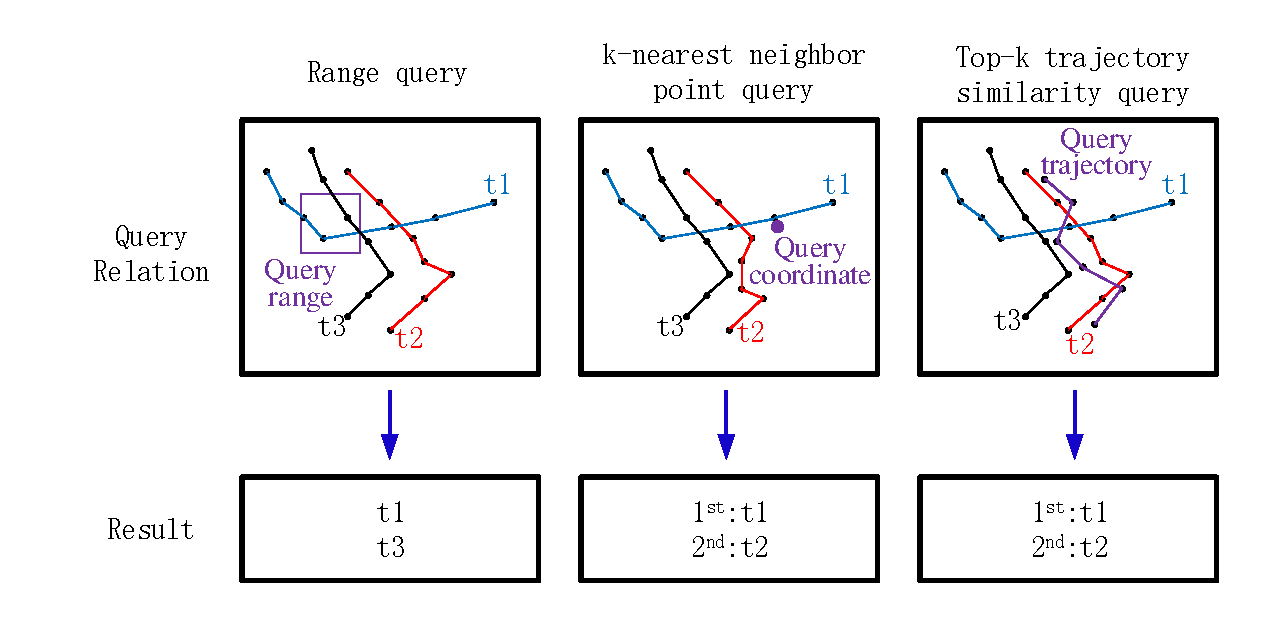
\includegraphics{querykind.pdf}
	%	\caption{three kind of query\label{fig:1}}
	%	\end{figure*}
	
	\begin{definition}[Top-k Similarity Query]
		Given a trajectory $t_q$, the $k$ value and the trajectory dataset $\mathbb{D}$, the top-k similarity query $TSQ(t_q,k,\mathbb{D})$ is defined as:
		\begin{equation}
		\begin{split}
		TSQ(t_q,k,\mathbb{D}) = &  T_s\subseteq \mathbb{D} \; s.t. \; \forall t_1 \in \mathbb{D}/T_s , \forall t_2 \in T_s, \\ &EDR(t_q,t_2) \leq EDR(t_q,t_1),|T_s|=k
		\end{split}
		\end{equation}
	\end{definition}
}

\subsection{Parallel Programming for GPUs}

\noindent{\bf GPU architecture and programming model.}
%
A GPU typically consists of tens of Streaming Multiprocessors (SMs) where each SM includes a number of cores running threads concurrently. All threads execute the same set of instructions over different data, following the Single Instruction Multiple Data (SIMD) parallelism model. Each SM has its local memory and 64 or 128 cores, and all SMs share global memory, establishing a complicated memory hierarchy.
Data requested by threads must be transferred from main memory to global memory first, via PCIe bus (the bandwidth is lower than 10GB/s).

We adopt CUDA~\cite{nvidia2014toolkit} proposed by NVIDIA as our programming model over GPUs. A GPU program is also referred to as a \emph{kernel}. When executing a kernel program, a grid of CUDA threads are launched immediately. We divide all CUDA threads into blocks and further into warps explicitly. During GPU computing, each CUDA block will be assigned to one SM which maintains a warp scheduler to determine which warp to be executed over the cores in next clock cycle. 



\noindent{\bf Challenging issues in GPU programming.}
%
The performance of a GPU program can be affected by the following factors. 

(1) \emph{DRAM-global memory data transfer.}
The capacity of global memory in GPU is too limited to keep a large number of trajectories, thus requiring frequent data transfer between main memory and global memory via PCIe bus. However, the high latency and low bandwidth of PCIe bus may easily become the bottleneck of the GPU program. We notice that when executing a batch of queries, the data to be accessed may overlap. Hence, it is desirable to develop a checking method to avoid redundant data transfer. 

(2) \emph{Global memory access pattern.}
When the data accessed by different threads in the same warp resides continuously in the global memory, the responding requests can be coalesced into a few data transactions. Otherwise, a large number of individual requests are issued, which increase the required global memory bandwidth significantly.



(3) \emph{Load balance.}
It is important to assign similar computational workloads to different GPU SMs. In particular, an SM with heavier workload may become a straggler, hindering the overall performance.

All the above factors pose great challenges in developing GPU-accelerated approaches to trajectory query processing. We will show how our framework addresses these challenges in the following sections.




\eat{
	We develop \frname based on CUDA~\cite{nvidia2014toolkit} proposed by NVIDIA, which is a popular programming framework for GPU computing. To  we introduce some background of GPU programming in the context of CUDA. 
	
	GPU follows Single Intruction Multiple Data (SIMD) parallelism model, indicating all of the cores in an Stream Microprocessor (SM) executing the same instruction on different data at the same time. There are tens of SMs in one GPU, each of which has 32 or 64 cores, forming a two-level parallel architecture. In CUDA, this architecture is reflected in the division of CUDA grid, CUDA block and CUDA thread. When one program is loaded in CUDA, a grid including mass of CUDA blocks is generated. Each CUDA block contains a fixed number of CUDA threads, which execute the same instruction in parallel. A SM execute some CUDA blocks, while each core of SM runs a CUDA thread of that CUDA block. The CUDA threads within the same CUDA block share a low volume but low latency local memory, while all CUDA threads in a CUDA grid share a global memory, whose latency is higher but capacity is larger. This special architecture of GPU requires us to divide the task properly into different CUDA blocks. There are three main issues when using GPU.
	
	\noindent \textbf{Memory Access Pattern} It is important to access the global memory in a proper pattern. If the bytes accessed by hundreds of threads are nearby in global memory, hundreds of data transactions generated by these threads will be coalesced into several large data transactions. Because the high bandwidth but high latency feature of global memory, this coalescing reduce the data fetching time significantly. For example, if thread 0 - 31 access the data at offset 32 - 63 respectively, 32 data fetching transactions will be combined into a transaction. In our framework, we aim to achieve this coalesce access pattern when designing the index and the procedure of query processing.
	
	\noindent \textbf{Load Balance} To best utilize GPU to achieve a high throughtput, the load balance should be achieved to make sure that all cores are not idle. This issue requires the task assigned to each CUDA block should has a similar scale in our framework.
	
	\noindent \textbf{Data Transfer and Store} The capability of GPU global memory is limit, and meanwhile the bandwidth of PCI-E is much lower than that of global memory, which proposes a dilemma between storing all data in main memory and global memory. Meanwhile, this requires us to reduce data transferring through PCI-E to avoid the performance loss. 
	
	Comparing to other parallel computing tools based on multi-core CPU such as MPI, these three issues raise a challenge for \frname to get a high speedup ratio on GPU.
}

\section{\frname Framework}\label{sec:framework}

\begin{figure}[t]
	\centering
	\includegraphics[width=\linewidth]{pdf/Architecture_V4.pdf}
	\caption{\frname Framework}\label{fig:arch}
\end{figure}

Figure~\ref{fig:arch} provides an overview of our \frname framework, which consists of two components: offline pre-processing and online trajectory query processing.

\subsection{Offline Pre-processing}

There are two main steps in this component:

\noindent $\bullet$ {\bf Building global grid and reorganizing trajectory points}:
As discussed in Section~\ref{sec:intro}, our index structure depends on cell-level trajectory representation. This is archived by constructing a squared \emph{global grid} covering all the trajectory points. We divide this grid into $4^\lambda$ disjoint \emph{cell}s in the same size along the two geospatial coordinates, where $n$ can be pre-defined to control the total number of cells and point density per cell. Given raw trajectories, we map each trajectory point to its covering cell accordingly. All the points in the same cell are sorted by their belonging trajectory ids and timestamps in ascending order. Let $\allcell$ denote all the cells in the global grid and $P(C)$ denote a sequence of points residing in cell $C\in \allcell$.

\noindent $\bullet$ {\bf Building \idxname index}:
Our index structure contains two parts: PR-quadtree~\cite{DBLP:conf/gis/LettichOS15} and cell-based trajectory table, both of which are connected to a grid of cells as mentioned above.
PR-quadtree organizes uniform cells into coarse-grained \emph{block}s. Each leaf node in PR-quadtree corresponds to a block. While the number of cells in each block differs, the number of the involving trajectory points per block is similar. This benefits load balance for range query processing. The cell-based trajectory table is used to reconstruct trajectories from cell data, which facilitate efficient processing of top-$k$ similarity queries.

\subsection{Online Trajectory Query Processing}

Without loss of generality, we illustrate the major steps of trajectory query processing by considering a single query. The processing of a batch of queries is independent and concurrent.
We first introduce how to perform trajectory range query, which involves two steps. 

\noindent $\bullet$ {\bf Candidate block generation}:
The input to this step is a query region $R$ and the output is a set of blocks (i.e., each block contains several cells) involving candidate trajectory points, denoted by $\rangecand$. To do this, we first traverse PR-quadtree in \idxname to locate leaf nodes in which the corresponding blocks are overlapped with $R$. 
We then identified the block as a candidate block and put into $\rangecand$, and check if points within it are already retained in global memory of GPU. If not, the points in that block are transferred into GPU and corresponding item in MAT is updated.
\eat{
We then check if the block is already retained in global memory of GPU. If not, the block is identified as a candidate block and put into $\rangecand$.
}

\noindent $\bullet$ {\bf GPU-accelerated point refinement}:
In this step, we verify all the points in the candidate blocks $\rangecand$ using GPU. If a point resides in $R$, we retrieve the corresponding trajectory based on trajectory id and add it into the final result set $\rangeq(R)$. For load balance purpose, we assign a block of trajectory points to one GPU SM for verification. 
Each CUDA thread is responsible for several points in the same block, while nearby points in global memory are verified by nearby threads to achieve a coalesce access pattern and increase data access throughput.
\eat{
Each CUDA thread is responsible for several continuously stored points in the same block to increase data access throughput.
}

To handle trajectory top-$k$ similarity query, we maintain a $k$-sized priority queue $PQ$ in main memory and perform the following three steps, where step 2 and 3 are executed iteratively.

\noindent $\bullet$ {\bf Frequency distance (FD) computation}:
The input to this step is a query trajectory $T$ and a positive integer $k$.
In this step, we compute a lower bound of $\edr(T, T')$ for each $T'\in \alltraj$, which will be used for pruning unnecessary EDR computation. To derive a lower bound, we follow the approach proposed by~\cite{} that calculates frequency distances first. However, applying FD computation in cell granularity can be time-consuming when the number of cells is large. We address the problem by constructing a virtual grid scheme to make a tradeoff between pruning power and FD computation cost.


\noindent $\bullet$ {\bf Candidate trajectory generation}:
In each iteration of this step, we select a set of trajectories with the smallest EDR lower bounds, because they are more likely be to the top-$k$ answers. We reconstruct these candidate trajectories, denoted by $\simcand$, from a grid of cells.

\noindent $\bullet$ {\bf GPU-accelerated ERR computation}:
In each iteration, the input to this step is query trajectory $T$ and several candidate trajectories $\simcand$. We distribute EDR computation tasks among CUDA blocks uniformly and the each state in every independent step within the computation is performed by each CUDA thread. Due to the high computation cost of EDR, we propose a parallel algorithm to further improve the performance. 

In the end of each iteration, we insert candidate trajectories into priority queue $PQ$ based on their EDR values. The iteration terminates when (1) $PQ$ contains $k$ trajectories, and (2) none of the candidate trajectories in the current iteration has lower EDR value than the tail trajectory in $PQ$.


\eat{
	In this section, we introduce the overview of our framework briefly. Our framework has three main components: storage component, range query processing and top-k similarity query processing.
	
	
	
	\subsection{Storage Component}
	There are two main steps in this component:
	
	\noindent \textbf{Generating Global Grid and Splitting Trajectories}
	We firstly build a grid and then split trajectories into it. Given the raw trajectory dataset $\mathbb{D}$, we detect the range of coordinates of whole dataset to set a square area. Based on this area, a fixed grid $G$ called Global Grid which contains $4^{\lambda}$ cells is built, acting as the base of \idxname index. After that, the trajectories in $\mathbb{D}$ are split according to the $G$, and points within each cell $c_i$ are accumulated to a data block $b_i$ with some $tID$ tags distinguishing which trajectory the points belong to. 
	%The frequency vectors of trajectories in $\mathbb{D}$ are also generated in this step.
	
	\noindent \textbf{Constructing PR-Quadtree}
	The load balancing is strongly required in GPU computing. To achieve this characteristic, we build a PR-quadtree \cite{DBLP:conf/gis/LettichOS15} $QT$ based on $G$ in which cells are linked to each node according to the location, with a constrain that for each node $N_i$, the number of points within the cells linked to it does not exceed a given threshold $M_{node}$. Morton-based encoding is performed to the identifies of cells for the purposes including coalesce access pattern and fast traverse of quadtree, and the characteristic of it permits us to get the identifies of cell directly from a coordinate. Finally, a memory allocated table (MAT) recording which data block retained in global memory is initialized and maintained to avoid duplicated data transferring from main memory to GPU, which use a LRU strategy to cache the data blocks.
	%Our system includes two parts, storage component and query processing component. As the Figure \ref{fig:Archi} shows, raw trajectories are preprocessed and divided into sub-trajectories according to quadtree index, with the corresponding sequence of cell stored as cell-based trajectories. After raw trajectories are loaded into storage component, thousands of queries are processed in query processing component, with the acceleration of GPU, outputing query results. It's worth noting that our system is designed for query-only applications, and we do not concern about the manipulation of data after building index. We then introduce these two components briefly.
	
	\subsection{Range Query Component}
	There are two main steps in this component:
	
	\noindent \textbf{Candidate Blocks Generation}
	In this step, a set of MBRs of queries $MBR_q$ is given and the output is a set of data blocks $\mathbb{B}_q$ called candidate blocks. This step consists two substeps. Firstly, for each MBR $mbr_i$ in $MBR_q$, a set of overlapped nodes $N_i$ is retrieved from \idxname. Next, the data blocks $B_i$ corresponding to the cells linked to these nodes are added to $\mathbb{B}_q$ and checked if they retain in global memory. Data blocks not in global memory are then transferred into it to be ready for the refinement. 
	
	\noindent \textbf{GPU-accelerated Points Refinement}
	In this step the candidate blocks in $\mathbb{B}_q$ are verified whether the points in them are within the corresponding MBR, and a set $tID$ which has points within given MBR is produced. Each data block is assigned to a CUDA block, and a CUDA thread checks several points in this data block whether they are within MBR. 
	
	%In the design of storage component, we exploit the potential oppotunities of quadtree with Morton encoding~\cite{DBLP:conf/gis/LettichOS15} with the consideration of GPU and propose an index called GT-quadtree. We divide all trajectories into sub-trajectories with small cell, after which each cell in quadtree is related to a set of sub-trajectories. To rebuild the whole trajectory from sub-trajectories easily, we propose a data structure named "cell-based trajectories" for each trajectory, storing the cell's identification it goes through, according to its original order. All data are stored in host memory, because in our strategies it is CPU that executes pruning process. The detail of storage component will be introduced in Section IV.
	
	\subsection{Top-k Similarity Query Component}
	In this component, a priority queue $PQ$ and a candidate set $\mathbb{C}$ are maintained for each query, storing the current top-k result and trajectories whose EDRs have been calculated respectively for this query. The frequency distance is firstly calculated, then the loop of candidate trajectories generation and GPU-accelerated EDR calculation continues until none of trajectories in $\mathbb{D}\backslash \mathbb{C}$ can be chosen as the candidate.
	
	\noindent \textbf{Frequency Distance (FD) Calculation}
	Given a query trajectory $t_q$, to prune unneccessary EDR computation, the FDs between $t_q$ and trajectories in dataset $\mathbb{D}$ are calculated as the lower bound of EDR in this step. We use the generated FVs and leverage an algorithm proposed in ~\cite{DBLP:conf/sigmod/ChenOO05} to calculated the FDs for all queries. Considering that this calculation may be time-consuming when the number of cells is large, we propose a virtual grid scheme to make a tradeoff between pruning power and computational cost of FDs.  
	
	\noindent \textbf{Candidate Trajectories Generation}
	In this step, $l$ candidate trajectories $t_c$ with lowest FD are extracted from $\mathbb{D}$ for each query trajectory $t_q$, because they are more likely to be the top-k result. After that, these trajectories are reconstructed according to corresponding cell-based trajectory and transferred into global memory.
	
	\noindent \textbf{GPU-accelerated EDR calculation}
	The input of this step is a set of candidate trajectories $T_c$ and the query trajectory $t_q$. The EDR between $t_q$ and each $t_c \in T_C$ are calculated in parallel by GPU, then they are inserted to the priority queue $PQ$ and correspondding candidate trajectories are inserted to $\mathbb{C}$.
	
	%Our query engine is designed for handling thousands of queries including two basic kinds in parallel, optimizing for executing time per query. Different kinds of queries are executed in different query components, based on the same storage component. In both two query components, we use GT-quadtree index to filter the candidates, then accelerate refinement by leveraging GPU. We will illustrate query engine in Section V.
}

\section{Spatial Index for Trajectory Queries}\label{sec:index}
In this section, we describe our spatial index \idxname developed for answering trajectory queries with GPUs.

%We firstly introduce the index structure, and then the process of index construction. 

\subsection{Structure of \idxname}

% Index performs as an important role in storage system by pruning unnecessary accessing of data. However, existing works about index on trajectories can not be easily used to solve our problem. First, in previous researches about trajectory storage system, different kind of query need different type of index, because of different characters of pruning strategies. Pruning on range query and k-nearest neighbor point query concern more about the relation between one query location and a trajectory. On the other hand, pruning on top-k similarity query concerns about the relation between two trajectories, which are sequences of locations, make it differentiated from two kinds of queries mentioned. Second, as mentioned in background, programming framework of CUDA raises a mass of claims about storage.


Grid-based spatial indices are known to have low construction/maintained costs and facilitate effective pruning for range and similarity queries~\cite{}. 
Our index \idxname is thus developed based on a squared \emph{global grid}, covering all the trajectories. In our design, we simply partition the grid into $4^\lambda$ cells of the same size along two geospatial coordinates, which can be visualized into a $2^\lambda \times 2^\lambda$ cell matrix (see Figure~\ref{}).
Each cell $C$ has an identifier $cid$, which is determined by the Morton-based encoding method~\cite{}.
As mentioned in Section~\ref{sec:framework}, we denote by $\allcell$ the set of cells.

%We associate each cell $C\in\allcell$ with an identifier $cid$, which determines the

Based on a grid $\allcell$ of cells, we develop our spatial index \idxname following a two-part structure: cell-based trajectory table and PR-quadtree. Figure~\ref{fig:Index} shows our index structure.

%introduce part1
\noindent {\bf Cell-based trajectory table $\trajtable$}.
This table is used to store all trajectories in cell-level representation. We adopt such representation to facilitate pruning strategies for both range and similarity queries. 
We also associate the table with a trajectory index to reconstruct any trajectory efficiently. 
To get cell-level representation for any trajectory in $\alltraj$, we map each trajectory point to its covering cell. 
We then define a cell-based trajectory table $\trajtable$ as a sequence of cells ordered by cell identifiers, i.e., $C_1\rightarrow\cdots\rightarrow C_{|\allcell|}$, where $C_i.cid < C_{i+1}.cid$ for $i\in[1,|\allcell|-1]$.
Within a cell $C\in\allcell$, we keep all the trajectory points belonging to it, denoted by $P(C)$, in ascending order of (trajectory id, timestamp).
In this manner, $\trajtable$ stores points from the same trajectory in each cell continuously in memory.

To reconstruct raw trajectories, we maintain a trajectory index over $\trajtable$. The index maps a trajectory id $tid$ to a vector $L_{tid}$. Each element in $L_{tid}$ is a triplet of ($cid, offset, length$), representing a subsequence of the raw trajectory $T_{tid}$. Specifically, $offset$ and $length$ specify a continuous part in $\trajtable$, which contains all the points from trajectory $T_{tid}$ that are within cell $C_{cid}$. By traversing vector $L_{tid}$, we are able to obtain all the points in trajectory $T_{tid}$. Note that the size of $L_{tid}$ is typically smaller than the number of trajectory points, especially when the points from a trajectory are aggregated into a few cells.
We illustrate an example of $\trajtable$ in Figure~\ref{fig:Index}... [give an example?]

\begin{figure}[t]
	\centering
	\includegraphics[width=\linewidth]{pdf/Index_V2.pdf}
	\caption{The \idxname Index\label{fig:Index}}
\end{figure}

%introduce part2

\noindent  {\bf PR-quadtree $\quadtree$~\cite{}}.
While cell-based trajectory table provides a way to organize trajectory data, it is easy to see that the number of points per cell may differ greatly. 
%Intuitively, cells in central areas of a city can have high point density and those in remote areas may contain zero point. 
Such differences result in imbalanced workload on GPU during query processing (see details in Section~\ref{sec:query}). To alleviate the problem, we leverage PR-quadtree~\cite{DBLP:conf/gis/LettichOS15} to group cells into coarse-grained \emph{node}s.

PR-quadtree can be pruned from a complete-quadtree $QT$. As figure~\ref{fig:Index} shows, based on Global Grid, we can organize all cells of $G$ in a $QT$ in which each leaf node is corresponding to a cell. We can see the depth of $QT$ is $\lambda+1$, because there are total $4^\lambda$ cells in $G$. In each level of $QT$, each node $N=(nid,level,isLeaf,block)$ is assigned with an ID $nid$ according to the ascending order from 0. The level of the node $level$ from 0 and a binary label $isLeaf$ indicating whether the node is leaf or not are also stored in each node. Each node has a $block$ corresponding to $4^k$ cells, where $k=\lambda + 1 - level$. 
In $QT$, the ID of cells in $N.block$ can be computed from $N.nid$ through binary shifting operations, according to the theorem~\ref{theo:nodeToCell}.

\begin{theorem}{\label{theo:nodeToCell}}
	Given Node $N=(nid,level,isleaf,block)$, the set of the ID of cells corresponding to $N$ is:
	$$block=\{4^{\lambda-level}\times nid + j|j\in \mathbb{N},0\leq j< 4^{\lambda-level}\}$$
\end{theorem}

For example, ...[give an example?]

PR-quadtree is generated by \textit{merge} some nodes in $QT$. We first define the operation ``merge'' to the node $N$ of $QT$:
\begin{definition}[merge]\label{def:merge}
	Given a non-leaf node $N$ in $QT$, a merge operation indicates:
	(1) drop all the daughters of $N$;
	(2) set $N.isLeaf$ to $TRUE$.
\end{definition}

From $QT$, we scan the nodes $N$ in the same level and merge them from level $\lambda$ to the level 1 if following rules are satisfied:
(1) $N$ is a non-leaf node;
(2) all the daughters of $N$ are leaf nodes;
(3) the total number of points within all the cells $c\in N.block$ is less than a given parameter $M_{node}$.

After this process, the complete-quadtree $QT$ is transformed into a PR-quadtree $\quadtree$. It can be easily seen that PR-quadtree satisfies the theorem~\ref{theo:Mnode}.

\begin{theorem}\label{theo:Mnode}
	Let $LN$ be any leaf node of $\quadtree$, the total number of points within all the cells $c\in LN.block$ is less than $M_{node}$.
\end{theorem}


We define two operations for traversing PR-quadtrees: $findParent$ and $findDaughter$.
\begin{definition}[findParent]\label{def:findParent}
	Let $N=(nid,level,isLeaf)$ be a node of PR-quadtree $\quadtree$ where $level>0$, $findParent$ is a map from the node $N$ to another node $N_p$, where $N_p.level=N.level-1$ and $N_p.nid=\lfloor N.nid/4\rfloor$.
\end{definition}

\begin{definition}[findDaughter]\label{def:findDaughter}
	Let $N=(nid,level,isLeaf)$ be a node of PR-quadtree $\quadtree$ where $isLeaf=FALSE$, $findDaughter$ is a map from the node $N$ to a set of node $N_D$, in which all $N_d\in N_D$ satisfy: $N_d.level=N.level+1$ and $N.nid=\lfloor N.d/4\rfloor$.
\end{definition}

From these two definitions, we can see that PR-quadtree can be traversed by binary shifting operations, which means the pointers among nodes are not neccessary when storing it, reducing the memory cost in implementation. For example, ...[give an example?]


%PR-quadtree is a $4$-ary tree, where the root node represents the global grid. Each node $N$ in the tree has several attributes: the node level $l$ in the tree, the node id $nid$ within the level, and a binary label $isleaf$ indicating whether the node is leaf or not. Each node $N$ corresponds to a virtual block $B_N\subseteq\allcell$ containing a set of cells. A node $N$ can have $4$ child nodes if we split the block $B_N$ uniformly by two coordinates.
%One can easily see that in PR-quadtree, (1) any two nodes following the ancestor-descendant relationship satisfy the spatial inclusive policy, i.e., $B_{N_1}\subseteq B_{N_2}$ iff $N_1$ is a descendant of $N_2$; (2) any cell in $\allcell$ belongs to exactly $1$ leaf node.

\noindent {\bf Benefits of \idxname}.
%summarize the benefits of two parts.
There are three main benefits of \idxname:
% cell-based trajectory table can recover the whole trajectory and FV, which are very useful information when choosing candidates in similarity query
(1) Cell-based trajectory table $S$ provides the cell-based trajectories, which is very useful when recovering whole trajectories from $\trajtable$ and calculating the lowerbound of EDR when running similarity query. For range query, $\trajtable$ stores trajectories according to the cells continuously, meaning that it is convenient to achieve coalesce access pattern during the refinement of candidates.
% quadtree leads to the load balancing for range query
(2) Through PR-quadtree, we can leverge theorem~\ref{theo:Mnode} to achieve a load balanced task division for range query processing, which is an important issue of improving the throughtput of GPU.
% coalesce access pattern because of the continuous cells in a node
(3) Also, according to theorem~\ref{theo:nodeToCell}, cells corresponding to the same node have continuous ID, so in $\trajtable$ the data of the points in these cells are nearby. This is benefical for achieving coalesce access pattern during the refinement on GPU.

\subsection{Construction of \idxname}
As the index for the query on historical data, the index is constructed before all query processing starting. In this section, we illustrate the procedure of constructing the index. The procedure is shown in Algorithm 1.

\begin{algorithm}[t]
	\algsetup{linenosize=\tiny}
	\scriptsize
	\caption{Index Construction}
	\label{alg:constr_index}
	\begin{algorithmic}[1]
		\REQUIRE ~~\\
		Global Grid $\allcell$; Trajectory Dataset $\mathbb{D}$; parameters $M_{node}$, $\lambda$;
		\ENSURE ~~\\
		Cell-based Trajectory Table $\trajtable$; PR-quadtree $\quadtree$;
		\FOR{$t\in \mathbb{D}$}
			\STATE $SEG \leftarrow splitTraj(t,\allcell)$
			\FOR{$s \in SEG$}
				\STATE $cid \leftarrow getCID(s)$
				\STATE $offset \leftarrow \allcell[cid].insert(s.points)$
				\STATE $\trajtable.L[t.tid].insert(triplet(cid,length(s),offset))$
			\ENDFOR
		\ENDFOR
		\STATE $QT \leftarrow buildCompQuadTree(\allcell,\lambda,\trajtable)$
		\FOR{$level$ from $\lambda-1$ to $0$}
			\FOR{$nid$ from $0$ to $4^{level}-1$}
				\STATE $merge(locateNodeInQuadTree(level,nid))$
			\ENDFOR
		\ENDFOR
		\STATE $\quadtree \leftarrow QT$
		\RETURN $\trajtable,\quadtree$
	\end{algorithmic}
\end{algorithm}

Cell-based Trajectory Table $\trajtable$ is built during building global grid $\allcell$. Trajectories in the dataset are split into a set of segments $SEG$ according to $\allcell$. For each trajectory whose ID is $tid$, a segment $s\in SEG$ contains points within the same cell $C$, and they are inserted into $P(C)$. Meanwhile, a triplet $(cid,num,offset)$ is appended into the $L_{tid}$, where $cid$ is the identify of $C$, $num$ is the length of $s$ and $offset$ is the offset of the first point of $s$ in $P(\allcell)$. After processing all trajectories, the construction of $\trajtable$ is finished.

In next step we construct the PR-quadtree. Firstly a complete-quadtree $QT$ is built based on $\allcell$.
The root node $root$ of $QT$ is initialized with $level=0$ and $cid=0$, corresponding to all cells of $\allcell$ in $block$. The descendant nodes of $root$ are generated recursively, whose procedure is shown in algorithm \ref{alg:buildQT}. During generating descendant node $N_{des}$ of $N$, the cells in four quandrants of $N$ are divided into four sets, then they are inserted to the $block$ of four daughters respectively. (line 5 - 8) According to the Definition~\ref{def:findDaughter}, $level$ and $cid$ can be directly computed, which are used to locate and insert $N_{des}$ into $QT$. (line 9) If $N_{des}.level$ is equal to $\lambda$, it will be set as a leaf node and the daughters will not be generated, and in this situation there is only one cell in $N_{des}.block$.

After all descendant nodes of $QT$ are generated, the merge operations are performed to nodes of $QT$ from level $\lambda-1$ to level 0. Then the construction of PR-quadtree $\quadtree$ is finished.

\subsection{Space Requirements}
Let $N_t$ and $L_t$ represent the number and the average length of trajectories in $\mathbb{D}$. Given the parameter $\lambda$ and the average number of points within in a cell for one trajectory $M_{cell}$, assuming in the worst situation that PR-quadtree is a complete quadtree, the memory cost of \idxname can be calculated as equation (4).

\begin{equation}
	\begin{split}
		Cost(\idxname )=&4\times N_t\times L_t + 3\times \frac{L_t\times N_t}{M_{cell}}\\&+ 4^\lambda + 3\times \frac{4^\lambda -1}{3}
	\end{split}
\end{equation}

The first fraction is the cost of all data blocks, and four elements (longitude, latitude, timestamp and trajectory ID) need to be stored for a point. And it is also the cost of the raw trajectories. The second fraction represents the cost of cell-based trajectory table, because each node in it has three elements ($cid$, $number$, $offset$) and there are $\frac{L_t\times N_t}{M_{node}}$ nodes. In Global Grid, only an pointer of data block need to be stored, so the cost is $4^\lambda$. At last, there are $\frac{4^\lambda -1}{3}$ nodes in complete PR-quadtree, and in each node $level$, $id$ and $isLeaf$ are neccessary to be retained, so the last fraction represents the cost of PR-quadtree.

From above analysis, we can see space requirements are much smaller than trajectory dataset itself at a proper configuration. For example, in a dataset containing 100,000 trajectories with average length of 800 in a range of $51.2km\times 51.2km$, $\lambda = 9$ (the length of cell side is 100m), and $M_{cell}=10$, we can find raw trajectories need 1280MB to be stored, while in our framework the total memory consumption is 99+1280MB.
 
%Storage component construction starts initially with an empty fixed grid covering the whole spatial plane. We first set the length of each cell is set to $m$ times of specified noise threshold of EDR distance $\epsilon$. It make the cell equivelent as two-dimensional bin. Then we build a grid containing $4^{m}$ cells, to guarantee that we can build a quadtree on it. Identifiers of cells are assigned according to the rule of Morton encoding, as figure \ref{Grid} shows.
%
%After that, we split the input trajectories into sub-trajectories. For each trajectory, we allocate sample points to corresponding cell of the grid, in order of cell's identify one by one. Sample points within the same cell are stored continuously in sub-trajectory array, with the offsets of each trajectories are marked in the cell. In this process, we record the sequence of cells allocated, generating the cell-based trajectory. We transfer all cell-based trajectories to GPU global memory, forming the cell-based trajectory list. 
%
%Based on this fixed grid, similar with the method in ~\cite{DBLP:conf/gis/LettichOS15}, we build a new quadtree as our final index, in which the number of each cell not exceeding a given threshold $M_{cell}$, assuring load balancing when dividing range query into multiple tasks. In the process of building quadtree, we start with creating an empty root node which covers all of the cells as the root of quadtree, identified as (0,0). Then we calculate the volumes for all nodes in quadtree, which indicates the number of sample points the node contains. We say a node contains a sample point if this point is within the cell which this node covers. Then, nodes whose volume is larger than $M_{cell}$ will be divided into four quadrants, forming the children nodes in next level, meanwhile other nodes are labeled as leaf nodes, containing less than $M_{cell}$ points. This procedure will be invoked recursively until there is no node to be divided. For example, in figure \ref{GTQuadtree}, node (1,1) in \ref{NodesL1}is divided into (2,4), (2,5), (2,6) and (2,7) in \ref{NodesL12}.




\section{GPU-accelerated Query Processing}\label{sec:query}

In this section, we introduce the strategy of query processing of our framework on CPU-GPU hybrid environment. The goal is to handle both range queries and top-k similarity queries and get a high throughput. 

\subsection{Overview}

Various spatial indices increase throughput by pruning a considerable amount of computation in the query execution. However, the computational cost of refinement still occupies a large propotion in the execution time of query processing even if there is an efficient indexing scheme. In range query, millions of points wait to be verified after the filter phase under the situation of large-scale queries. This phenomenon is more obvious for top-k similarity query processing, because the complexity of calculating EDR is quadratic. In our experiment, only 10 top-5 similarity query on a 9GB dataset spends about 700s, although the state-of-the-art pruning scheme is applied.

It is an oppotunity to utilize GPU to accelerate the refinement phase in query processing. A straightforward method may be directly assigning each query task to a CUDA thread. However, this method cannot make full use of GPU because of some special issues mentioned in the background. For range query, different queries may have different area $R_q$ and different dense of points, which means the workloads of them are not balanced and leads to a low speedup. For similarity query, there exists some dependence between the procedure of calculating EDR. If we directly dispatch computational tasks to CUDA threads, a large amount of synchronization between them will make some cores idle during the computation and reduce the overall throughput. Moreover, the data placement and layout have big effects on the efficiency, because the requirement of coalesce access pattern and the low transferring speed between main memory and global memory.

To get a better usage of GPU under these issues, we design a series of strategies in query processing based on the storage component of \frname. In this section, they will be introduced through the illustration of how CPU and GPU work together and some details of implementation on GPU. We firstly introduce the procedure of range query and then following top-k similarity query.

\subsection{Range Query}
% (This part is simple and similar with work in other works, so use several sentence to describe.)

\begin{algorithm}[t]
	\algsetup{linenosize=\tiny}
	\scriptsize
	\caption{Range Query}
	\label{alg:RQ}
	\begin{algorithmic}[1]
		\REQUIRE ~~\\
		queryIDs $Q$; query ranges $R_Q$; dataset $\mathbb{D}$; PR-quadtree $\quadtree$, Cell-based Trajectory Table $\trajtable$;
		\ENSURE ~~\\
		Result Trajectories $T_{result}$;
		\STATE $C_P\leftarrow initTable()$
		\FOR{$q\in Q$ \textbf{parallelly}}
			\STATE $C_N,\rangecandnode \leftarrow initSet()$
			\STATE $C_N.insert(\quadtree.root)$
			\WHILE{$C_N\neq \phi$}
				\STATE $N\leftarrow C_N[0]$
				\STATE $A_R\leftarrow AR(R_q.mbr,N.level)$
				\STATE $CR_N\leftarrow CR(N)$
				\IF{$CR_N.N_x\in A_R.x_r$ \textbf{AND} $CR_N.N_y\in A_R.y_r$}
					\IF{$N.isLeaf=TRUE$}
						\STATE $\rangecandnode.insert(N)$
						\STATE $C_P.insert(pair(N,q))$
					\ELSE
						\STATE $DC\leftarrow findDaughter(N)$
						\STATE $C_N.insert(DC)$
					\ENDIF
				\ENDIF
			\ENDWHILE
		\ENDFOR
		\STATE $transferDatatoGPU(C_P,\trajtable)$
		\STATE $transferPairsToGPU(C_P)$
		\STATE ${Tid} \leftarrow verifyTrajOnGPU(R_Q,C_P)$
		\STATE $T_{result}\leftarrow recoverTraj(L_{Tid},\trajtable)$
		\RETURN $T_{result}$
	\end{algorithmic}
\end{algorithm}

Similar to the most of works about range query, we use a filter-and-refine scheme when processing range queries as Algorithm~\ref{alg:RQ} shows. Considering that there are a large amount controlling instructions such as judgement, looping and branching in the traverse of PR-quadtree, it is better to finish the filter phase by CPU because many divergences are generated in controlling instructions, which hurts the efficiency significantly (line 1-21). Tasks in refinement phase are almost computational operations, so this phase is accelerated by GPU in our framework (line 22-23).

%achieve this in two step. There have been a solution~\cite{GPUTaxi} leveraging GPU to handle range query based on quadtree. However, this solution is based on a fact that all the points will be transfered into GPU memory, which is not realistic at a big data scene. In our solution, by integrate a usage table technique, we can also achieve a similar speedup even if data are not all in GPU memory. 
%

\subsubsection{Filter by CPU}

In this phase a query ranges $R$ are input and candidate blocks $\rangecand$ are retrieved, then a set of candidate points $\rangecand$ are transferred to global memory, waiting for verifying in the refinement phase.

\begin{figure}[!t]\centering
	\scriptsize{
		\begin{minipage}{0.5\linewidth}
			\centering
			\includegraphics[width=\linewidth]{pdf/AR_lv2.pdf}
			(a) Example of procedure of $AR(mbr,2)$ in level 2
		\end{minipage}
		\hfill
		\begin{minipage}{0.46\linewidth}
			\centering
			\includegraphics[width=\linewidth]{pdf/MBR_lv2.pdf}
			(b) Example of procedure of $CR(N)$ in level 2
		\end{minipage}
	}
	\caption{Examples of the procedure $AR(mbr,l)$ (left) and $CR(N)$ (right)\label{fig:ARCR}}
\end{figure}

Given $mbr_R$, we can judge in each layer which nodes overlap the MBR. We firstly define a map $AR$ from MBR and level $l$ to a tuple of range. 

\begin{definition}[$AR(mbr,l)$]\label{def:AR}
	Given all the nodes in the level $l$ in a complete-quadtree $QT$, the area of Global Grid can be divided into an $2^l\times 2^l$ grid and coordinates in each axis are divided into $2^l$ ranges $R_X$ and $R_Y$ identified from 0 to $2^l-1$ respectively. Then, given an MBR $mbr=(x_{min},y_{min},x_{max},y_{max})$, the $AR(mbr,l)$ is defined as 
	$$AR(mbr,l)=(x_{R},y_{R}), ~s.t.$$
	$$x_{R}=\{R_X[i]|R_{X_{min}}\leq i\leq R_{X_{max}},~i\in \mathbb{N}\}$$
	$$y_{R}=\{R_Y[i]|R_{Y_{min}}\leq i\leq R_{Y_{max}},~i\in \mathbb{N}\}$$
	where $R_{X_{min}}$, $R_{X_{max}}$, $R_{Y_{min}}$, $R_{Y_{max}}$ are the range that $x_{min},y_{min},x_{max},y_{max}$ located respectively.
\end{definition}

Then we define the a map $CR(N)$ from $N$ to its ranges in x-axis and y-axis, called the \textit{range coordinate}.
\begin{definition}[$CR(N)$]\label{def:CR}
	Given node $N$ with ID $nid$ in the level $l$, $CR(N)$ is defined as:
	$$CR(N)=(N_x,N_y), ~s.t.$$
	$$N_x=\sum_{i\in N_{even},0\leq i\leq 2l-1}(\lfloor \frac{nid}{2^i}\rfloor \mod 2)\times 2^{\lfloor \frac{i}{2}\rfloor}$$ 
	$$N_y=\sum_{i\in N_{odd},0\leq i\leq 2l-1}(\lfloor \frac{nid}{2^i}\rfloor \mod 2)\times 2^{\lfloor \frac{i}{2}\rfloor}$$ 
\end{definition}


Figure~\ref{fig:ARCR}(a) shows an example of $AR(mbr,l)$ in level 2 of a complete-quadtree. $mbr$ is represented as the red dotted rectangle, and we could get the ranges in x-axis and y-axis that two vertexes locate in. After that, $x_R$ and $y_R$ can be calculated and output as the result of $AR(mbr,2)$.
Figure~\ref{fig:ARCR}(b) shows an example of $CR(N)$ in level 2 of a complete-quadtree. Given an cell `6', the range coordinate of it is $(10,01)_2$. It can be seen that these two maps are able to implemented by some trivial bit-wise operations with a low computational cost. 

Based on these definitions, we introduce the procedure of the filtering phase. We firstly maintain two sets $C_{N}$ and $\rangecandnode$, and add the root of PR-quadtree $\quadtree$ to $C_N$ (line 3-4). Then, for each $N\in C_{N}$, we generate $AR(R.mbr,N.l)$ as the $A_{R}$, and generate $CR(N)$ as the $CR_{N}$ (line 6-8). If $CR_N.N_x\in A_{R}.x_{R}$ and $CR_N.N_y\in A_{R}.y_{R}$, we say that $N$ \textit{overlap}s $R$. Then, if this $N$ is a leaf as well, it will be added to $\rangecandnode$, else the daughters of it are extracted by $findDaughter(N)$ and added to $C_{N}$ (line 9-17). This process terminates when $C_{N}=\phi$. Finally, $\rangecandnode$ is the set of all leaf nodes that overlaps the MBR of $R$.

\eat{
We traverse the PR-quadtree $\quadtree$ from the root, and for each $N$ we access, we  to the layer $\lambda$ to find leaf nodes whose block intersect or overlap the MBR $mbr_R$ of $R$. This process can be finished by several $findDaughter$ operations. 


Figure \ref{fig:MBR_FindCell}(a) shows the example of nodes in level 2 in a complete PR-quadtree. The coordinates of two vertexes are transformed to binary \{(00, 01), (10, 11)\}, then we can find that from the transformation shows at upper right, the ID of nodes containing two vertexes can be generated. Applying this transformation to the range of coordinates generated from MBR, as the table at lower right shows, we can generate all the nodes which the MBR overlap or intersect. In non-complete quadtree some ID of nodes may not exist, so these invalid IDs will then be eliminated. Another example of nodes in level 1 is shown in figure \ref{fig:MBR_FindCell}(b). 

For leaf nodes overlapping or intersecting $mbr_q$, they are added into the candidate set $Cand_q$. For the non-leaf nodes overlapping or intersecting $mbr_q$, we check their daughters recursively. The ID of daughters can be generated by applying a two-bit leftshift to the parent's ID, then adding ``00'', ``01'', ``10'', ``11''. For example, the daughters of $N=(1,2)$ can be found by equation (5).

\begin{equation}
	\begin{split}
		(1,2) &= (1,10_2)\\&\Rightarrow 
		\begin{cases}
			(2,1000_2) = (2,8)\\
			(2,1001_2) = (2,9)\\
			(2,1010_2) = (2,10)\\
			(2,1011_2) = (2,11)
		\end{cases}
	\end{split}
\end{equation}
}

For each query $q\in Q$ a $\rangecandnode$ can be generated parallelly in multiple threads of CPU, and we make the pair of node $N\in \rangecandnode$ and query $(N,q)$ and add it to a new table $C_P$. For each node $N$ in $C_P$, the cells in $N.block$ are searched and points of them are extract from cell-based trajectory table $\trajtable$ and transferred into global memory. Reminding that the number of points within a node is smaller than $M_{node}$, the tasks of verifying points in these pairs are in even scale. Finally, the information about table $C_P$ and the query ranges of $q\in Q$ denoted as $R_q$ are transferred into global memory.

\subsubsection{Refine by GPU}

\begin{algorithm}[t]
	\algsetup{linenosize=\tiny}
	\scriptsize
	\caption{verifyTrajOnGPU}
	\label{alg:verifyTrajRQ}
	\begin{algorithmic}[1]
		\REQUIRE ~~\\
		query ranges $R_Q$; table $C_P={pair(N,q)}$; Point Data $DB$;
		\ENSURE ~~\\
		Result Trajectories $T_{result}$;
		\FOR{$cudaBlockID \in [0,size(C_P)-1]$ \textbf{parallelly}}
			\STATE $blockDB \leftarrow DB[cudaBlockID]$
			\STATE $queryID \leftarrow C_P[cudaBlockID].q$
			\STATE $blockRange \leftarrow R_Q[queryID]$
			\FOR{$i\in [0,size(blockDB)/N_{thread}]$}
				\FOR{$cudaThreadId \in [0,N_{thread}-1]$ \textbf{parallelly}}
					\STATE $p \leftarrow blockDB[i*N_{thread} + cudaThreadID]$
					\IF{$p\in blockRange$}
						\STATE $T_{result}[queryID][p.tID]\leftarrow TRUE$
					\ENDIF
				\ENDFOR
			\ENDFOR
		\ENDFOR
		\RETURN $T_{result}$
	\end{algorithmic}
\end{algorithm}

At the second step, we refine the candidates on GPU in parallel and get the final results. The procedure is shown in Algorithm~\ref{alg:verifyTrajRQ}. Each CUDA block is assigned with a $(N,q)$ pair, which indicates a task of checking which points in the cells of $N.block$ are truely within the query range $R_q$. In each CUDA block, points are assigned evenly to CUDA threads in loops. As mentioned in \ref{sec:index}, points within the same cell are stored continuously, and the identifies of cells in a node are consecutive because of Morton-based encoding. For this reason, we propose an strategy that in a single loop, $N_{thread}$ threads verify $N_{thread}$ points in parallel, and the loop continues until all the points are verified. In this strategy memory request of the threads are nearby, so the coalesce accessing pattern is achieved. For example, in the first loop, thread 0 reads point 0, thread 1 reads point 1, and so on. In addition, reminding that the quantity of points within a node is smaller than $M_{cell}$ points, the load balance is achieved in this step. 

\subsubsection{Complexity Analysis}
We analyse the complexity of our approach of range query. Given the length of a cell $L_cell$, the density of points $\rho$, the number of cores in an SM $N_{core}$, the number of SM in a GPU $N_{SM}$, the parameter $M_{node}$ and the area of query range $S_q$, the overall computational cost is calculated as equation~\ref{eq:costRangeGPU}, while the cost on CPU approach is calculated as equation~\

\begin{equation}\label{eq:costRangeCPU}
	\begin{split}
		Cost_{RQ(CPU)} = \sum_{q=1}^{N_Q} \rho S_{q}
	\end{split}
\end{equation}


\begin{equation}\label{eq:costRangeGPU}
	\begin{split}
		Cost_{RQ(GPU)} = &\frac{\max \{\rho L^2_{cell}, M_{node},N_{core}\}}{N_{core}}\\ &\times \sum_{q=1}^{N_Q}  \frac{\rho S_{q}}{N_{SM} M_{node}}
	\end{split}
\end{equation}

% maybe it is not neccessary to analysis the cost of CPU.

\subsection{Top-k Similarity Query}

Given a query trajectory $T_q$, the goal of the top-k similarity query is retrieve k closest trajectories $\simq(T_q)$ measured by EDR. As shown in Algorithm~\ref{alg:TSQ_1}, the FDs between $T_q$ and trajectories $T_d\in \alltraj$ are firstly calculated as the lower bound of EDR, then we iterate between generating candidates and calculating real EDRs in batch, until none of the candidate trajectories in current iteration has lower possible EDR value than the trajectories whose EDRs have been calculated. 

\subsubsection{Frequency Distance Calculation}

In this component, we firstly use cell-based trajectory table $CT$ in \idxname to generate the frequency vectors (FV) of $T_q$ and $T_d$, which indicate the number of points within each cell for a trajectory. For trajectory $T_d\in \alltraj$, because in $L_d\in \alltraj$ there is a value $num$ storing the number of points belonging to trajectory $T_d$ within each cell, we can get its FV $FV_d$ through a scan in $L_d$. This step can be performed during offline pre-processing, because FVs of $T\in \alltraj$ will be reused many times during large-scale similarity query. For query trajectory $T_q$, owing to the Morton-based encoding of Global Grid, given the point sequence of $T_q$ including coordinates, the identifies of cells that the points reside in can be computed using method shown in figure x. So, we can generate FV $FV_q$ easily as well.

After $FV_q$ and $FV_d$ are generated, the FD $FD(FV_q,FV_d)$ between them can be calculated by CompHisDist algorithm\cite{DBLP:conf/sigmod/ChenOO05} with linear complexity. According to the Theorem~\ref{theo:LB}~\cite{DBLP:conf/sigmod/ChenOO05}, $FD(FV_q,FV_d)$ is the lower bound of $EDR(T_q,T_d)$.

\begin{theorem}\label{theo:LB}
	Let $T_r$ and $T_s$ be two trajectories, $FV_r$ and $FV_s$ be the frequency vector of $T_r$ and $T_s$ respectively. We have $FD(FV_r,FV_s)\leq EDR(T_r,T_s)$.
\end{theorem}

However, FV will be very long if $\lambda$ of Global Grid is big because of large number of cells, and in this situation the cost of computing FD is high, although the complexity of ComHisDist algorithm is linear. For example, in Shanghai private cars dataset, an area of $51.2\times 51.2 km^{2}$ is divided into $2^18$ cells, if the length of a cell is set as $100m$. Inspired by the solution about alter the granularity of histogram proposed in ~\cite{DBLP:conf/sigmod/ChenOO05}, we build a Virtual Grid $\allcell_V$, in which the number of cells is smaller than Global Grid, to reduce the length of FV. Under our \idxname index, we do not need extra memory to store virtual grid because the information of it can be obtained by computation directly. 

The virtual grid can be seen as all of nodes in one layer of complete-quadtree, so we can use $findParent$ operation of range query to obtain the corresponding ID of cell in $\allcell_V$ for the cell in $\allcell$. Figure \ref{fig:VirtualGrid} is an example: a virtual grid with 4 cells is built based on a fixed grid with 16 cells. Chen~\cite{DBLP:conf/sigmod/ChenOO05} has proved that FD is a looser lower bound of EDR as long as the length of cell in grid is the multiple of $\epsilon$. So, FV can be redefined as the number of points within each cell in virtual grid, and under this definition FD is looser lower bound of EDR but cheaper to be computed. We set a parameter VC, which indicates $\lambda-i$, to control this tradeoff: 

if we use the virtual grid to calculate FD, the cost of computation will decrease. Owing to the Morton encoding of GT-quadtree, the virtual grid can be used without the requirement of extra memory consumption, because we can directly get which cell in the virtual grid contains a given point and then generate FVs. For example, in figure \ref{fig:VirtualGrid}, the original FV of the trajectory can be simplified into [1,5,0,0], whose length is decreased from 16 to 4, just by a transformation implemented by right shifting. However, it should also be pointed out that a tradeoff should be found between too large and too small cells because the larger cells are, the looser bound is. We set a parameter called VC permitting the configuration of this tradeoff, which indicates how many right shifting operations are performed to get the transformation from original FV to simplified one in virtual grid. In above example, the VC parameter is 2.

% For a trajectory $t_i$ within the corresponding cell,  whose cell-based trajectory $L_i$ has $m$ nodes, we maintain an length-$m$ array $V_{freq}$ and initialize it to all-zero firstly. Then, we get the sequence of cells from $L_i$, and for each node $(cid,num,offset)$ we add $num$ to the cid-th value of $V_{freq}$. After processing the whole $L_i$, the array $V_{freq}$ becomes the FV of trajectory $t_i$. The FV of $t_q$ and $t_d$ can be generated by this method, and then the FD between them are calculated by CompHisDist algorithm\cite{DBLP:conf/sigmod/ChenOO05} with linear complexity.



\subsubsection{Candidate Generation}

Based on the FD between $T_q$ and all $T_d\in \alltraj$, we generate the candidates which are likely to be the one of top-k closest trajectories of $T_q$ in every loop and then invoke GPU to calculate the real EDR between $T_q$ and them to reduce the times of complex EDR calculation.

We use a xxx scheme in the process of candidate generation with the lowerbound FD to make sure that there are no trajectories probable to be one of the results are omitted. We firstly maintain a priority queue $FDPQ$ to store the FDs between $T_q$ and all trajectories of $\alltraj$, with all calculated FDs together with the trajectory ID added into it. Then, in each iteration, different from traditional xx scheme which chooses one candidate once, we extract $l>1$ trajectories whose FDs are the smallest from $FDPQ$ to a candidate set $Cand_q=(T_{c},T_q)$ waiting for calculating real EDR, because in traditional situation the scale of candidates is small, while GPU can only get a remarkably high speedup under a large number of tasks. After $Cand_q$ is extracted, the candidate trajectories $T_{c}$ in it are recovered with the help of $CT$ form cell-based trajectory table and transferred into global memory of GPU, together with the information about $T_q$ and some parameters such as $\epsilon$ needed in the calculation of EDR. At the end of this iteration, the tasks of calculating EDR between each $T_c$ and corrsponding $T_q$ are uniquely assigned to CUDA blocks. 






\begin{algorithm}[t]
	\algsetup{linenosize=\tiny}
	\scriptsize
	\caption{Top-k Similarity Query}
	\label{alg:TSQ_1}
	\begin{algorithmic}[1]
		\REQUIRE ~~\\
		Query trajectory set $T_q=\{t_{q_i}|0\leq i< size(T_q)\}$; Cell-based Trajectory Table $\alltraj$; k value $k$; EDR parameter $\epsilon$;
		\ENSURE ~~\\
		Top-k Result $Result_{T_q}=\{result_i|0\leq i< size(T_q),result_i=\simq(t_{q_i})\}$
		\FOR{$i\in [0,size(T_q)-1]$ \textbf{parallelly}}
			\STATE $Vq_{freq}\leftarrow generateFVFromTraj(t_{q_i})$
			\STATE $FDPQ_q\leftarrow initPriorityQueue()$
			\STATE $EDRPQ_q\leftarrow initPriorityQueue()$
			\FOR{$L_j \in \alltraj$}
				\STATE $V_{freq_j}\leftarrow generateFV(L_j)$
				\STATE $FDPQ_i.push(j,calculateFD(V_{freq_j},Vq_{freq}))$
			\ENDFOR
		\ENDFOR
		\STATE $isFinished \leftarrow initArray(FALSE,size(T_q))$
		\WHILE{$isFinished$~is~not~all~$TRUE$}
			\STATE $candPair=[]$
			\FOR{$i\in [0,size(T_q)-1]~AND~(!isFinished[i])$ \textbf{parallelly}}
				\STATE $Cand_q\leftarrow popLowest(FDPQ_i)$
				\FOR{$key\in Cand_q$}
					\STATE $t_{key}\leftarrow recoverTraj(L_{key},G)$
					\STATE $candPair.insert(key,i)$
					\STATE $transferTrajtoGPU(t_{key})$
				\ENDFOR
				\STATE $transferTrajtoGPU(t_{q_i})$
			\ENDFOR
			\STATE $EDR_{result}\leftarrow calculateEDRbyGPU(candPair,\epsilon)$
			\FOR{$result\in EDR_{result}$}
				\STATE $qID\leftarrow result.qid$
				\STATE $EDRPQ_{qID}.push(result.tid,result.EDR)$
				\STATE $isFinished[qID]\leftarrow checkFinish(FDPQ_{qID},EDRPQ_{qID})$
			\ENDFOR
		\ENDWHILE
		\RETURN $EDRPQ.popLower(k)$
	\end{algorithmic}
\end{algorithm}

\eat{
The goal of the top-k similarity query is generating the result of top-k similarity queries in a short time, leveraging the parallel power of GPU. We use EDR as the similarity measurement, which is popular and performs well in most of recent works. ~\cite{EDWP15}[] Our work can be migrated to other measurements whose calculation is based on dynamic programming algorithm, such as LCSS~\cite{DBLP:conf/icde/VlachosGK02}. However, considering that GPU efficiency is low if the task load is small, it is suboptimal to directly migrate algorithm proposed by ~\cite{DBLP:conf/sigmod/ChenOO05} to GPU, because this algorithm execute only one EDR calculation after a filter phase. As a solution, we adapt this algorithm to fit with GPU architecture and design a new filter and refine scheme, which is shown in Algorithm \ref{alg:TSQ_1}. The initial idea of this scheme is filtering some trajectories which can be assured not appearing in the result to avoid unnecessary expensive EDR computing. 

First, for each query, we use cell-based trajectories to calculate the lower bounds of EDR between query trajectory and trajectories in storage and add all trajectories to candidate set (line 3-5). After that, we find $\eta$ trajectories from candidate set whose lower bounds are the lowest, calculating the real EDR between query trajectory. Obtaining the upper bound of current top-k EDR distance of trajectories efficiently is a frequent operation for pruning, so a size-k priority queue of real EDR distance is maintained to handle this operation. (line 7-8). We then prune trajectories in candidate set whose lower bound is bigger than upper bound of current top-k EDR distance safely because we can assure they will never be chosen in following iterations (line 9). We repeat this process of choosing top-$\eta$ trajectories from candidate set and pruning until candidate set is empty. Finally trajectories in the priority queue are results of this top-k similarity query.
	
	
There is some challenges of performance in our proposed algorithm 1. In the most setting in actual situation, the number of cells are usually large, making the computation of lower bound a time-consuming process. For example, in Shanghai private cars dataset, an area of $45\times 55 km^{2}$ is divided into $247500$ cells, if threshold $\epsilon$ in EDR is set as $100m$. Besides, although through filtering, massive expensive EDR computations are still neccessary to execute. Attention that the computation cost of EDR between two trajectories is O($mn$)(m is the length of trajectory 1 and n is the length of trajectory 2), an efficiency issue arises as the length of trajectories become longer. 

To overcome these challenges, we use GPU to accelerate EDR calculation with GT-quadtree. However, this migration is not trivial because of the special architecture and programming model of GPU. Aiming to overcome these challenges and get better performance, we will introduce our strategies and implementation in detail at following part of this section.


\subsubsection{Lower Bound Generation}
% candidate set and priority queue, calculate lower bounds in parallel.
\begin{figure}[t]
	\centering
	\includegraphics[width=0.48\linewidth]{pdf/VirtualGrid.pdf}
	\caption{An example of virtual grid with 4 cells and the transformation between IDs in different grids\label{fig:VirtualGrid}}
\end{figure}

The lower bound of EDR can be derived from cell-based trajectories. This process is proposed in ~\cite{DBLP:conf/sigmod/ChenOO05}. We first generate frequency vector (FV) for each trajectory, storing the sample points the trajectory has in each cell. For example, in figure \ref{fig:VirtualGrid}, suppose the depth of GT-quadtree is 3. For a trajectory whose cell-based trajectory is [1,4,4,5,7,7,7], its frequency vector would be [0,1,0,0,2,1,0,3,0,...] of length 16. Frequency distance (FD), defined as the edit distance between two FVs, has close relationship with EDR between two corresponding trajectories. It is easy to find that insert, delete and replace operations in EDR is similar to adding one, subtracting one and subtracting one in one element then adding one in other element on FV correspondingly. But one adjacent case is special. If there is an replace operation between two adjacent elements of FV, indicating these two corresponding cells are adjacent in grid, it may cause one unnecessary operation in EDR. For example, given two FVs, $v_{1}=<1,0,0,0>$, $v_{2}=<0,1,0,0>$, and corresponding trajectories $R_{1}=(t_{1},0.9)$, $R_{2}=(t_{2},1.1)$ and $\epsilon =1$, replace operation is needed in FD but unnecessary in EDR. So, we can derive that FD is the lower bound of EDR.

Although the calculation cost of FD is lower than EDR, it still spends lots of time. There are two reasons. One is there are lots of trajectories in storage and for each of them an FD should be calculated. The other is if a small $\epsilon$ is set by user, the length of FV will be very long, causing even one FD is also computational cost. Aiming to these two issues, we proposed the strategies respectively. Firstly, widely used multicore CPU allows us to distribute the FD computation workload of all queries to different cores evenly, and then the calculation of all FD can finish in shorter time because the tasks are divided. Secondly, for the FD computation in each query, inspired by a solution proposed in ~\cite{DBLP:conf/sigmod/ChenOO05}, we build a virtual grid, in which the length of cell is larger than that of GT-quadtree's fixed grid, to reduce the length of FVs. It is trivial to execute FD calculation of different queries by using multithreading technology, so we then introduce the virtual grid in detail. 

The virtual grid can be seen as all of nodes in one layer of GT-quadtree. Figure \ref{fig:VirtualGrid} is an example: a virtual grid with 4 cells is built based on a fixed grid with 16 cells. Chen~\cite{DBLP:conf/sigmod/ChenOO05} has proved that FD is still the lower bound of EDR as long as the length of cell in grid is the multiple of $\epsilon$, no matter how large it is. So, if we use the virtual grid to calculate FD, the cost of computation will decrease. Owing to the Morton encoding of GT-quadtree, the virtual grid can be used without the requirement of extra memory consumption, because we can directly get which cell in the virtual grid contains a given point and then generate FVs. For example, in figure \ref{fig:VirtualGrid}, the original FV of the trajectory can be simplified into [1,5,0,0], whose length is decreased from 16 to 4, just by a transformation implemented by right shifting. However, it should also be pointed out that a tradeoff should be found between too large and too small cells because the larger cells are, the looser bound is. We set a parameter called VC permitting the configuration of this tradeoff, which indicates how many right shifting operations are performed to get the transformation from original FV to simplified one in virtual grid. In above example, the VC parameter is 2.
}

\subsubsection{GPU-accelerated EDR calculation}
% introduce how to calculate EDR in parallel on GPU
% include different size strategy, task generation, data transferring and data arrangement.
After generating lower bound FD and candidate generation, a mass of EDR calculations tasks $et=(d,q)$ are waited for executing. Each EDR calculation takes in two inputs trajectories $T_{d}$ and $T_q$, and output the EDR distance between them. For executing massive EDR calculations in parallel, the key is to finding an approach of dividing the each calculation process into independent sub-processes. Considering the strong independence among the task of different $traj_d$, we assign an EDR calculation taks to each CUDA block in block-level. Another benefit of this block-level division is that we can use low-latency local memory to store some frequently reused information such as points of trajectory within each task, which is helpful for improving throughtput. 

% firstly introduce traditional computation method, then point out problem and propose our approach
The original procedure of EDR calculation is similar to that of classical edit distance, according to the defination of EDR which is given in defination~\ref{def:edr}. A state matrix $S$ is maintained, and $S[i][j]$ is calculated by comparing and choosing the minimun value of $\{S[i-1][j]+1,S[i][j-1]+1,S[i-1][j-1]+subcost\}$. The elements of $S$ are calculated line by line and after all the elements have been calculated, the $S[m][n]$ is the EDR between two trajectories. However, in this procedure, there is a strong relationship amont calculation steps, which means that they cannot be directly mapped to the threads in the CUDA block. For example, when we calculate the states in line 3, $S[3][3]$ is relational to $S[3][2]$.
\eat{
\begin{figure}[t]
	\centering
	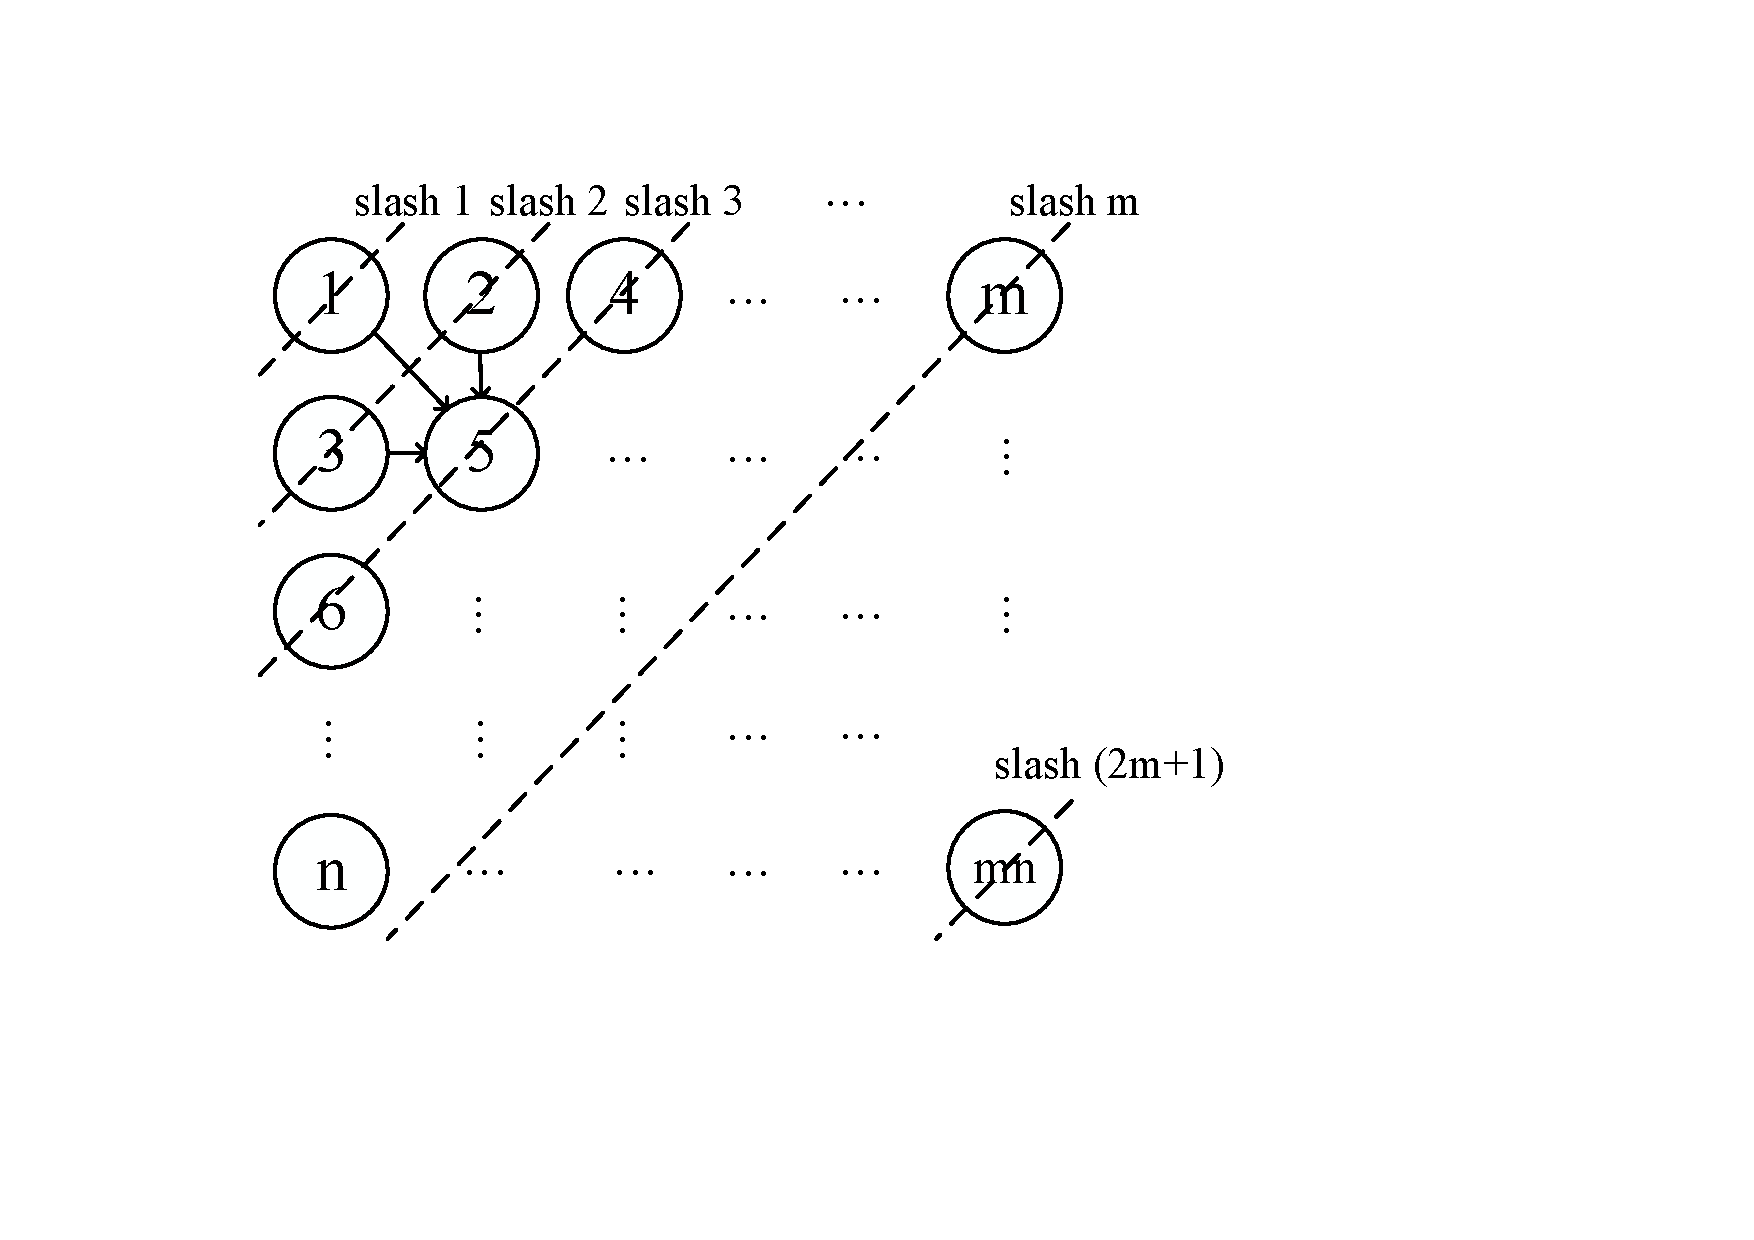
\includegraphics[width=0.48\linewidth]{pdf/DPstate.pdf}
	\caption{An example of EDR calculation procedure\label{fig:DPstate}}
\end{figure}
}

\begin{figure}[t]
	\centering
	\scriptsize{
		\begin{minipage}{0.34\linewidth}
			\centering
			\includegraphics[width=\linewidth]{pdf/StateMatrixDP_V2.pdf}
			(a) Relationship between states on different slashes 
		\end{minipage}
		\hfill
		\begin{minipage}{0.62\linewidth}
			\centering
			\includegraphics[width=\linewidth]{pdf/EDR_fetch.pdf}
			(b) Location of data each thread reads and writes
		\end{minipage}
	}
	\caption{An example of EDR calculation procedure\label{fig:EDR}}
\end{figure}

To solve this problem, we analyse the data dependency of original calculation procedure, finding that if we group the states on the same slash together in state matrix, the value of every state only relies on the states of the last two slashes, and meanwhile the calculations of states in the same slash are independent. Figure \ref{fig:EDR}(a) shows an example. When we calculate the states 7, 8, 9 and 10 on slash 4, only the states 4, 5, 6 on slash 3 and states 2, 3 on slash 2 are needed. 

Based on this observation, we propose an iterative procedure of the parallel EDR calculation in each CUDA block. For a task that $|traj_{d}|=m$ and $|traj_q|=n$, an $(m+1)\times (n+1)$-sized state matrix is maintained. In $i$-th iteration, thread $th_j$ calculate the $j$-th state on slash $i$ based on the corresponding states on slash $i-1$ and slash $i-2$. To achieve a coalesce access pattern, we store state matrix $S$ with xxx order (the order shows in figure \ref{fig:EDR}(b)), because based on this origanization values that threads read and write in each iteration are nearby. For example, on 4-th iteration, the read and write requests of threads 0-3 are continuous, contributing to the coalesce access pattern. For slashes which there are thousands of states on them, states are computed by all threads in some loops. Although not all CUDA threads work in iterations before calculating states on slash $N_{core}$, we argue that they have a small propotion of all iterations, because trajectories usually are longer than 200 meaning that there are usually more than 400 iterations in total, while $N_{core}$ is 64 or 128 on most of GPU. Therefore, a reasonble load balance is achieved in our iterative procedure.

\begin{algorithm}[t]
	\algsetup{linenosize=\tiny}
	\scriptsize
	\caption{Parallel EDR Calculation}
	\label{alg:EDR}
	\begin{algorithmic}[1]
		\REQUIRE ~~\\
		Two sets of trajectories: $\mathbb{T}_D,\mathbb{T}_Q$; Tasks information $Cand_q$; Threshold of EDR: $\epsilon$; Number of threads in a CUDA block $N_{thread}$
		\ENSURE ~~\\
		All EDR distance between trajectories in two sets: $EDR(T_{q},T_{d})$, $\forall (T_{q},T_{d})\in \{Cand_q|\forall q\in Q\}$
		
		\STATE Assign each $(T_d,T_q)$ pair to a thread block
		\STATE Initial an array to store results of all pairs assigned: $result[size(Cand_q)]$
		\FOR{CUDA block $bID$ \textbf{parallelly}}
			\STATE Initial matrix $S$ in global memory: $S[len(T_q)+1][len(T_d)+1]$
			\STATE $maxLen \leftarrow max(len(T_q),len(T_d))$
			\STATE Load trajectories in local memory: $Tq[len(T_q)]$, $Td[len(T_d)]$
			\STATE $slashNum \leftarrow len(T_q)+len(T_d)+1$
			\STATE $loopPerThread \leftarrow \lceil maxLen/N_{thread}\rceil$
			\FOR{slash $i$ from 1 to $slashNum$}
				\FOR{thread $tID$ \textbf{parallelly}}
					\STATE $sl_1 \leftarrow getSlashOffset(i-1)$
					\STATE $sl_2 \leftarrow getSlashOffset(i-2)$
					\FOR{each loop $j$ from 0 to $loopPerThread-1$}
						\STATE $sID\leftarrow j*threadNum+tID$
						\STATE $s_1 \leftarrow getUpState(sl_1,tID,j)$
						\STATE $s_2 \leftarrow getLeftState(sl_1,tID,j)$
						\STATE $s_3 \leftarrow getCrossState(sl_2,tID,j)$
						\STATE $subCost\leftarrow geneSubCost(Tq,Td,\epsilon)$
						\STATE $tempState[loopPerThread]\leftarrow min(s_1,s_2,s_3+subCost)$ 
					\ENDFOR
				\ENDFOR
				\FOR{each thread $tID$ \textbf{parallelly}}
					\FOR{each loop $j$ from 0 to $loopPerThread-1$}
						\STATE $sl_{now}\leftarrow getSlashOffset(i)$
						\STATE $sl_{now}[N_{thread}*j+tID]\leftarrow tempState[j]$
					\ENDFOR
				\ENDFOR
			\ENDFOR
			\STATE $EDR(T_q,T_d)\leftarrow S[len(T_q+1)][len(T_d+1)]$
		\ENDFOR
		\RETURN $EDR(\mathbb{T}_d,\mathbb{T}_q)$
	\end{algorithmic}
\end{algorithm}

\eat{
We designed an iterative framework for parallel EDR calculation. According to the defination of EDR which is given in defination~\ref{def:edr}, the process of EDR calculation can be divided into several independent steps. Figure \ref{fig:DPstate} shows an example of calculating the EDR between two trajectorie $traj_q$ and $traj_d$ with length $m$ and $n$. Each value in a state (represented as $state[i][j]$) is calculated by comparing and choosing the minimun value of $\{state[i-1][j]+1,state[i][j-1]+1,state[i-1][j-1]+subcost\}$. After all the states have been calculated, the $state[m][n]$ is the EDR between two trajectories. If we use slashes to group the states, we notice that the values of states in one slash rely on the value of states in two upper left slashes. For example, in figure \ref{fig:DPstate}, if we want to calculate the states on slash 3, the states on slash 1 and slash 2 are needed. Meanwhile, comparing operations within a slash have no relationship, inspiring us to invoke the calculations within the same slash in parallel, forming the basic idea of our solution.

\begin{algorithm}[t]
	\algsetup{linenosize=\tiny}
	\scriptsize
	\caption{Parallel EDR Calculation}
	\label{alg:EDR}
	\begin{algorithmic}[1]
		\REQUIRE ~~\\
		Two sets of trajectories: $\mathbb{T}_D,\mathbb{T}_Q$; Tasks information $Cand_q$; Threshold of EDR: $\epsilon$; parameters  $\epsilon$, $N_{thread}$
		\ENSURE ~~\\
		all EDR distance between trajectories in two sets: $EDR(T_{q},T_{d})$, $\forall (T_{q},T_{d})\in \{Cand_q|\forall q\in Q\}$
		
		\STATE assign each $(T_d,T_q)$ pair to a thread block
		\STATE initial an array to store results of all pairs assigned: $result[size(Cand_q)]$
		\FOR{each CUDA block $bID$ \textbf{parallelly}}
			\STATE initial matrix $S$ in global memory: $S[len(T_q)+1][len(T_d)+1]$
			\STATE $maxLength \leftarrow max(len(T_q),len(T_d))$
			\STATE load trajectories in local memory: $Tq[len(T_q)]$, $Td[len(T_d)]$
			\STATE $slashNum \leftarrow len(T_q)+len(T_d)+1$
			\STATE $loopPerThread \leftarrow \lceil maxLength/threadNum\rceil$
			\FOR{each slash $i$ from 1 to $slashNum$}
				\FOR{each thread $tID$ \textbf{parallelly}}
					\STATE initial an array in GPU SM's register to store states calculated: $tempState[loopPerThread]$
						\FOR{each loop $j$ from 0 to $loopPerThread-1$}
							\STATE update $tempState[j*threadNum+tID]$ using states on last two slashes
						\ENDFOR
					\ENDFOR
				\FOR{each thread $tID$ \textbf{parallelly}}
					\FOR{each loop $j$, $j\in [0,loopPerThread-1]$}
						\STATE flush $lastTwoSlash[0][j*threadNum+tID]$ to $state$ in corresponding position
						\STATE $lastTwoSlash[0][j*threadNum+tID]\leftarrow lastTwoSlash[1][j*threadNum+tID]$
						\STATE update $lastTwoSlash[1][j*threadNum+tID]$ using $tempState[j]$
					\ENDFOR
				\ENDFOR
			\ENDFOR
			\STATE $result[bID]\leftarrow state[len(t_1)][len(t_2)]$
		\ENDFOR
	\end{algorithmic}
\end{algorithm}

Based on this framework, we propose a procedure of calculating EDRs in parallel on GPU, as algorithm \ref{alg:EDR} shows, whose implement is based on CUDA. Given a set of EDR calculation tasks, we first assign each of them to a block to make GPU full-loading, in order to improve the throughtput(line 1-2). In each block, the values of states are calculated in $(2\times max\{m,n\}+1)$ loops from $state[0][0]$ to $state[m][n]$ slash by slash (line 10). For example, in figure \ref{fig:DPstate}, state on slash 1 is generated, and then slash 2, slash 3, ..., until the slash $(2m+1)$. In each loop data on two before slashes are stored in high-speed local memory of each SM, which is allocated before starting loops (line 6), because they will be frequently accessed by threads. Noting that the length of trajectory is almost smaller than 2048, it is enough for space of local memory to store these data. As for the state matrix of this calculation, we store them according to the order of slash, as figure \ref{fig:DPstate} shows. In this case, the data required by threads are nearby, assuring the coalesce accessing pattern.





In each thread block, based on the data of previous two slashes, all the values on current slash are calculated by mass of threads in parallel by equation (1) mentioned in Section II (line 11-16). After finishing the calculation on current slash i, the states on slash i-2 stored in local memory are flushed into state matrix in global memory, and then states on slash i-1 and i become the new "two last slashes" (line 17-22). The result of EDR calculation of this block can be extracted from state matrix after all loops (line 25). 

We can see that in our solution, the number of steps needed for EDR?calculation reduces from $mn$ to $(2max\{m,n\}+1)$ comparing to not using GPU, and this reduction could be so obvious if trajectory length $m$ or $n$ is large, which is usually an actual situation because the sample interval of location device is short, e.g. 2s.

% In each loop, states in two before slashes are stored as shared variables because in CUDA programming model all shared variables will be stored in high speed local memory and calculation of states on slash $i$ is related to states on slash $(i-1)$ and $(i-2)$. In this way all of states accessing transactions required from EDR calculation are from high speed local memory. In addition to this, we find that calculation of $state[i][j]$ needs for $traj_1[i]$ and $traj_2[j]$ and in some loops all of trajectory points are required. Also storing them as shared variables is surely a choice. However, for limited capabacity of local memory, this choice will impact the efficiency of GPU. This is because in GPU architecture, each SM can execute at most 8 blocks therotically at a time but all of shared variables of blocks are needed to be resident in local memory. So abusement of shared variables may limit the number of blocks running on an SM at the same time. For this reason, we choose 

\begin{algorithm}[t]
	\algsetup{linenosize=\tiny}
	\scriptsize
	\caption{Parallel EDR Calculation}
	\label{alg:EDR}
	\begin{algorithmic}[1]
		\REQUIRE ~~\\
		Two sets of trajectories: $T1,T2$
		
		Threshold of EDR: $\epsilon$
		
		Parallel parameters: $blockNum$, $threadNum$
		\ENSURE ~~\\
		all EDR distance between trajectories in two sets: $EDR(t_{1},t_{2})$, $\forall (t_{1},t_{2})\in T1\times T2$
		
		\STATE assign each $(t_1,t_2)$ pair to a thread block
		\STATE initial an array to store results of all pairs assigned: $result[blockNum]$
		\FOR{each block $bID$ \textbf{parallelly}}
		\STATE initial a matrix in global memory to store all states: $state[len(t_1)+1][len(t_2)+1]$
		\STATE $maxLength \leftarrow max(len(t_1),len(t_2))$
		\STATE initial a matrix in local memory to store states in last two slashes: $lastTwoSlash[2][maxLength+1]$
		\STATE $lastTwoSlash[0][0]=0$
		\STATE $slashNum \leftarrow len(t_1)+len(t_2)-1$
		\STATE $loopPerThread \leftarrow \lceil maxLength/threadNum\rceil$
		\FOR{each slash $i$, $i\in [1,slashNum]$}
		\FOR{each thread $tID$ \textbf{parallelly}}
		\STATE initial an array in GPU SM's register to store states calculated: $tempState[loopPerThread]$
		\FOR{each loop $j$, $j\in [0,loopPerThread-1]$}
		\STATE update $tempState[j*threadNum+tID]$ using states on last two slashes
		\ENDFOR
		\ENDFOR
		\FOR{each thread $tID$ \textbf{parallelly}}
		\FOR{each loop $j$, $j\in [0,loopPerThread-1]$}
		\STATE flush $lastTwoSlash[0][j*threadNum+tID]$ to $state$ in corresponding position
		\STATE $lastTwoSlash[0][j*threadNum+tID]\leftarrow lastTwoSlash[1][j*threadNum+tID]$
		\STATE update $lastTwoSlash[1][j*threadNum+tID]$ using $tempState[j]$
		\ENDFOR
		\ENDFOR
		\ENDFOR
		\STATE $result[bID]\leftarrow state[len(t_1)][len(t_2)]$
		\ENDFOR
	\end{algorithmic}
\end{algorithm}


%% ??????kernel?????????????????GPU????
%% ??????kernel?????????????????GPU????
%% ??????kernel?????????????????GPU????
We propose a multi-GPU implementation of our strategy dealing with large-scale of EDR calculation from all top-k trajectory queries by dividing the set of EDR calculation tasks into several equal size part, to achieve a load balancing and maximum usage of multiple GPUs. Before running these tasks, we use an independent memory allocated table (MAT) to store trajectory data when they are loaded into GPU global memory first, because in this way if a trajectory has been loaded into global memory, by looking for MAT we can avoid the duplicated low-speed data transfering between memory and GPU. However, the volume of the GPU global memory is usually so limited that not all trajectory data can be filled into it. To make an tradeoff, we maintain a memory pool and integrate it to MAT. If the pool is full, we use Least Recently Used (LRU) algorithm to drop some outdated trajectories. This strategy is efficient in real life because there exists hotspot within queries. For example, trajectories in city center may be required by queries more frequently because the population in city center is denser than rural area. After the kernel finishing, EDR calculation results from different GPUs are collected and query engine then filters the candidates, as shown in line 9 in algorithm \ref{alg:TSQ_1}.
}
\subsubsection{Complexity Analysis}
We finally analyse the complexity of our approach of top-k similarity query. We define computing one state in EDR calculation as the unit of cost. Denoting $E$ as the set of all neccessary EDR calculation tasks and $eid$ is the ID of task in $E$, for original EDR calculation algorithm on CPU, the total time cost is: 
\begin{equation}
Cost_{EDR(CPU)} = \sum_{e=1}^{len(E)} len(E[e].T_q)*len(E[e].T_d)
\end{equation}

Denoting $N_{SM}$ and $N_{core}$ as the number of SMs in GPU and cores in an SM respectively, the total time cost of our algorithm on GPU is:
\begin{equation}
\begin{split}
Cost_{EDR(GPU)} = &\sum_{e=1}^{len(E)} \{\frac{\lceil \frac{len(E[e].T_q)}{N_{core}} \rceil + \lceil \frac{len(E[e].T_d)}{N_{core}} \rceil}{N_{SM}}\times\\& [len(E[e].T_q)+len(E[e].T_d)]\}
\end{split}
\end{equation}

Under a typical condition that $N_{core}=128$,$N_{SM}={16}$ and $len(T.q)=len(T.d)=600$, we can see that the cost of original EDR calculation algorithm is 360,000, while that in our approach is 750. Although the frequency of cores on GPU is lower than CPU, a remarkble speedup can be obtained by our approach.


\section{Optimization}\label{sec:optimization}

\subsection{Less Data Transfer}

It is low efficient if duplicated data are transfered from host to GPU global memory, so we maintain a table recording the nodes whose data remain in GPU global memory and its corresponding pointer. Based on this technique, we first check whether the data of node are in GPU global memory. Only if neccessary, we transfer data of this node to GPU, otherwise the pointers of data are directly used to locate the required data. It is worth noting that CPU continue traversing the GT-quadtree simultaneously when transfering data, which can hide the latency caused by low-speed PCI to some extent. 

\section{Experiment}\label{sec:exp}
In this section, we conduct a multiview experiment based on two real trajectory datasets to verify the performance of GTS. We first introduce the experimental environment, then evaluate the efficiency and scalability of index, and compare the performance of two kinds of queries with baseline and state-of-the-art works at last.

\subsection{Experiment Setup}

\subsubsection{Dataset} We use two real life trajectory datasets which are collected from two largest cities of China respectively to test the performance in different trajectories distribution.

\noindent \textbf{SHCAR} SHCAR is the trajectories of some private cars in Shanghai City, which contains 327,474 trajectories and 75,188,293 sample points. Some extra information such as CARID, direction and OBD information are also included in this dataset. All the data were collected from July, 2014 to April, 2015. The sampling rate is about 10 seconds. The size of the raw data file is 8.96GB. 

\noindent \textbf{GeoLife} The GeoLife dataset is published by Microsoft Research Asia, which contains the trajectories from 182 users in a period from April 2007 to August 2012~\cite{DBLP:conf/www/ZhengZXM09}~\cite{DBLP:conf/huc/ZhengLCXM08}~\cite{DBLP:journals/debu/ZhengXM10}. We pick all the sample points within Beijing City, including 30,325 trajectories and 19,143,208 sample points. The size of raw data file is 2.11GB.

\subsubsection{Data Preprocessing} In our experiment, we seem the sequence of sample points of a the same car as a trajectory. If the difference between two time stamps of consecutive points is larger than 30 minutes in a trajectory, we call this point a "gap". We then split the trajectory into several new trajectories according to these gaps. This is because we usually only concern about the trajectory of a single route especially when handling similarity query, and trajectory with these gaps is usually not a meaningful single route. For example, a trajectory of a single car may include sample points from home to office and ones from office to home, and after spliting it two meaningful trajectories can be generated. After preprocessing we get at total 327,474 trajectories.

\subsubsection{Parameters} To systematically test the performance of our system, we conduct our experiments under various parameter settings. Table \ref{table_param} shows the range and default value of parameters we test in experiments. For range query, there are four parameters affecting the performance. In real life, queries from users vary from area, so we test for different size of MBB in range query. We also test the situations of different number of queries to evaluate the scalability of GTS. For top-k similarity search, the execution time under different k value and number of queries are recorded. As we show in section V the length of trajectory determines the complexity of EDR calculations so we test for different length to see whether GTS gets high performance at different situation. Size of cells are altered in all of experiments of both two kinds of queries.

\begin{table}[!t]
	% increase table row spacing, adjust to taste
	\renewcommand{\arraystretch}{1.3}
	% if using array.sty, it might be a good idea to tweak the value of
	% \extrarowheight as needed to properly center the text within the cells
	\caption{Parameters ranges and default values}
	\label{table_param}
	\centering
	% Some packages, such as MDW tools, offer better commands for making tables
	% than the plain LaTeX2e tabular which is used here.
	\begin{tabular}{|c||c|c|c|}
		\hline
		Parameter & Meaning & Range & Default\\
		\hline
		$L_{cell}$ & size of each cell in grid & 0.05 - 0.4 & 0.1\\
		\hline
		$M_{cell}$ & max num. of points in a cell & 256 - 4096 & 1024\\
		\hline
		$VC$ & the VC parameter of virtual grid & 1 - 50 & 15\\
		\hline
		$S_{RQ}$ & area of range query's MBR & 0.01 - 4 & 0.5\\
		\hline
		$k$ & k value of top-\textbf{k} similarity query & 8 - 128 & 32\\
		\hline
		$N_{Q}$ & num. of queries & 256 - 8192 & 1024\\
		\hline
		$L_{QT}$ & length of query trajectory & 256 - 8192 & 1024\\
		\hline
	\end{tabular}
\end{table}

\subsubsection{Baselines} For range query, we implement two state-of-the-art systems supporting range query on GPU: STIG~\cite{7498315} and FSG~\cite{GPUTaxi}. However, these two systems are designed facing to spatial-temporal points rather than trajectories, so we add a data field in each point to represent the trajectory ID of it. To show the acceleration performance, we also implement our approach on multicore CPU as the baseline method.

\noindent \textbf{STIG} This approach use kd-tree as the basic data structure, in which each leaf corresponds to a block rather than a point. We choose in-memory CPU-GPU hybrid strategy of it, which means when executing range query, kd-tree is firstly traversed by CPU and some candidate blocks are returned, then each block is refined by a block in GPU. We set the parameter of block size to 20000, same as default $M_{cell}$ in our approach.

\noindent \textbf{FSG} This approach leverage a flat grid-file based indexing to accelerate point-in-polygon queries for analysing taxi trip data. Similar to our approach, it firstly find cells which overlap the MBR of queries, then generate cell-polygon pairs and send them to GPU. In next phase each pair is processed by an SM, achieving the goal of acceleration. We set the parameter of size of cell to 0.02, same as default $L_{cell}$ in our approach. $R$ value is set to 0.0025.

\noindent \textbf{GTS-MCPU} The CPU version of GTS. In this approach each  $\langle node, query\rangle $ pair is assigned to a thread of CPU rather than an SM of GPU to achieve parallelism. All the parameters are set the same as which in GTS.
   
For similarity query, we only implement the original EDR-based top-k similarity query algorithm proposed in ~\cite{DBLP:conf/sigmod/ChenOO05} on multicore CPU as the baseline because as far as we know we are first to utilize GPU to accelerate EDR based top-k similarity query.

\noindent \textbf{EDR-MCPU} We modify original EDR-based top-k similarity query method to a multithread version by assigning each query task to a thread. The parameters of this method are the same as which in our approach.

\subsubsection{Experiment Overview} ???All other parameters are tuned to the optimal case.

After that, the scalability is tested. As there is no method to shut some cores in GPU, we can only test the situation with different number of GPUs.

In query performance part, same as the most of previous works, we use query latency as our metric. We compare the query time latency of two kinds of queries in different baselines and state-of-the-art systems in a large query set situation. When testing range query, we randomly generate range queries with different areas and positions and reckon the time consumption during finishing all of queries. To reflect the true working environment as much as possible, the chosen positions are restricted to the central district of Shanghai ($31.11^{\circ} N-31.36^{\circ} N, 121.39^{\circ} E-121.58^{\circ} E$). For similarity query, some trajectories are selected randomly from dataset as the query set. During the query, for each trajectory in query set, the result of top-$k$ similarity query is returned under the settings of different query parameters including $k$ and $\epsilon$. Queries are handled with formed query set and time consumption in both baseline method and GTS are then calculated. 


We run all the experiments on a server equipped with two ten-core Xeon E5-2650 v3 processor clocked at 2.3GHz, 64GB of RAM, 4TB of disk storage and an NVIDIA Tesla K80 GPU with 6GB graphical memory. Our system is implemented by C++ with CUDA 8.0, and operating system is CentOS 7.

\subsection{Query Latency}

In this section we evaluate the performance of range query and top-k similarity query under SHCAR dataset. For range query, we compare our approach with three baselines described in Section VI-A. For top-k similarity query, we only compare our system with the multicore-CPU implementation of original EDR based top-k similarity query because there is no other GPU-accelerated query processing approach based on EDR. 

\begin{figure}[!t]
	\centering
\scriptsize{
	\begin{minipage}{0.48\linewidth}
		\centering
		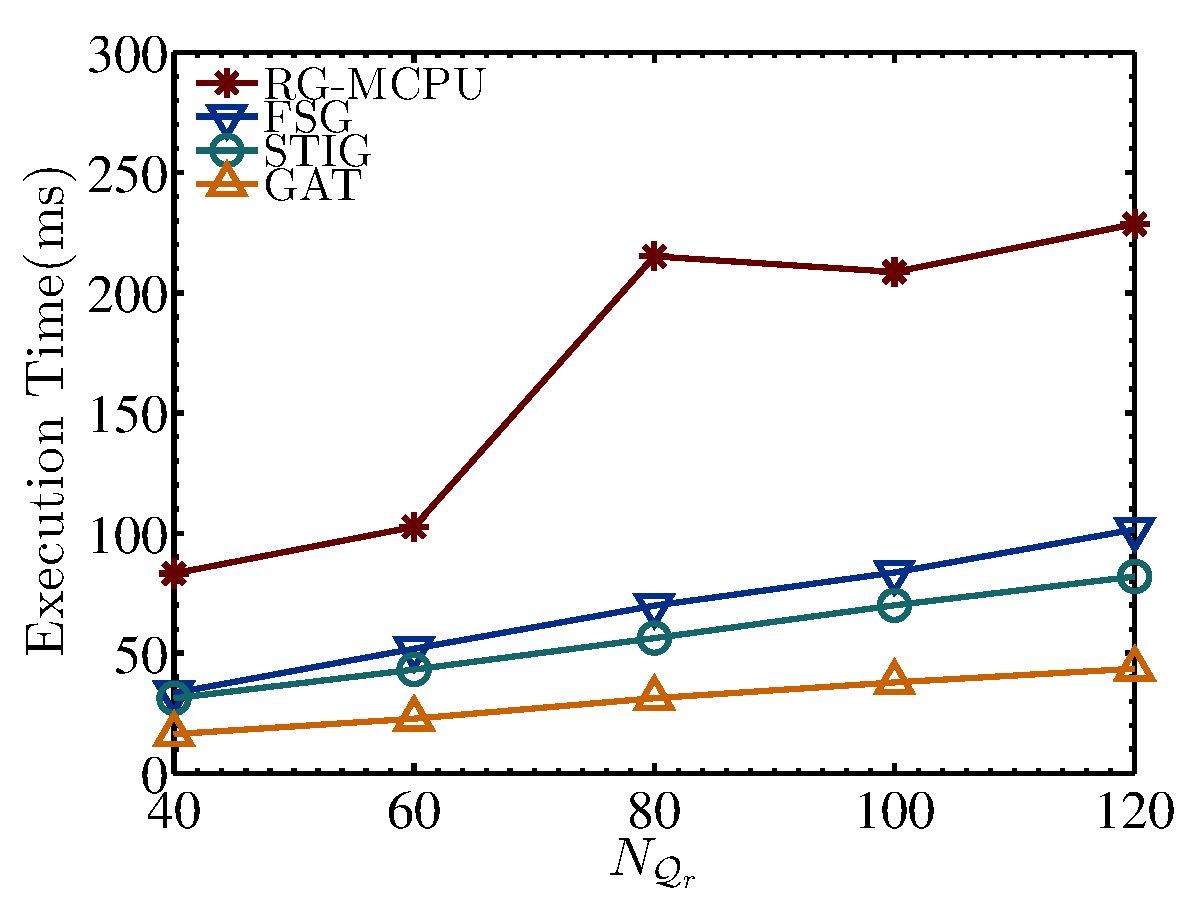
\includegraphics[width=\linewidth]{eps/QueryNum_RangeQ.eps}
		(a) Execution time for different number of range queries 
	\end{minipage}
	\hfill
	\begin{minipage}{0.48\linewidth}
		\centering
		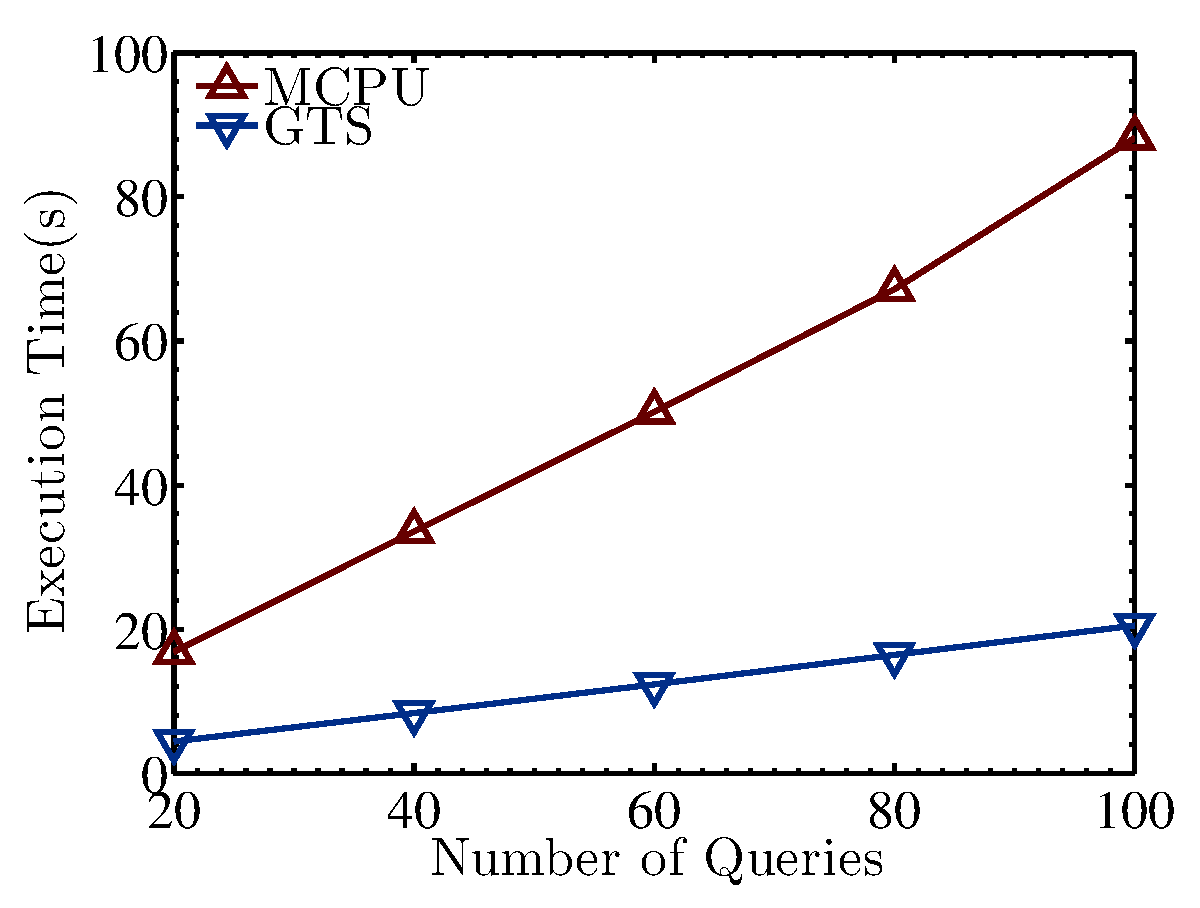
\includegraphics[width=\linewidth]{eps/QueryNum_SimilarityQ.eps}
		(b) Execution time for different number of top-k similarity queries
	\end{minipage}
}
	\caption{Query performance for range query and top-k similarity query under different workload\label{fig:QueryNum}}
\end{figure}

\begin{figure}[!t]\centering
	\scriptsize{
		\begin{minipage}{0.48\linewidth}
			\centering
			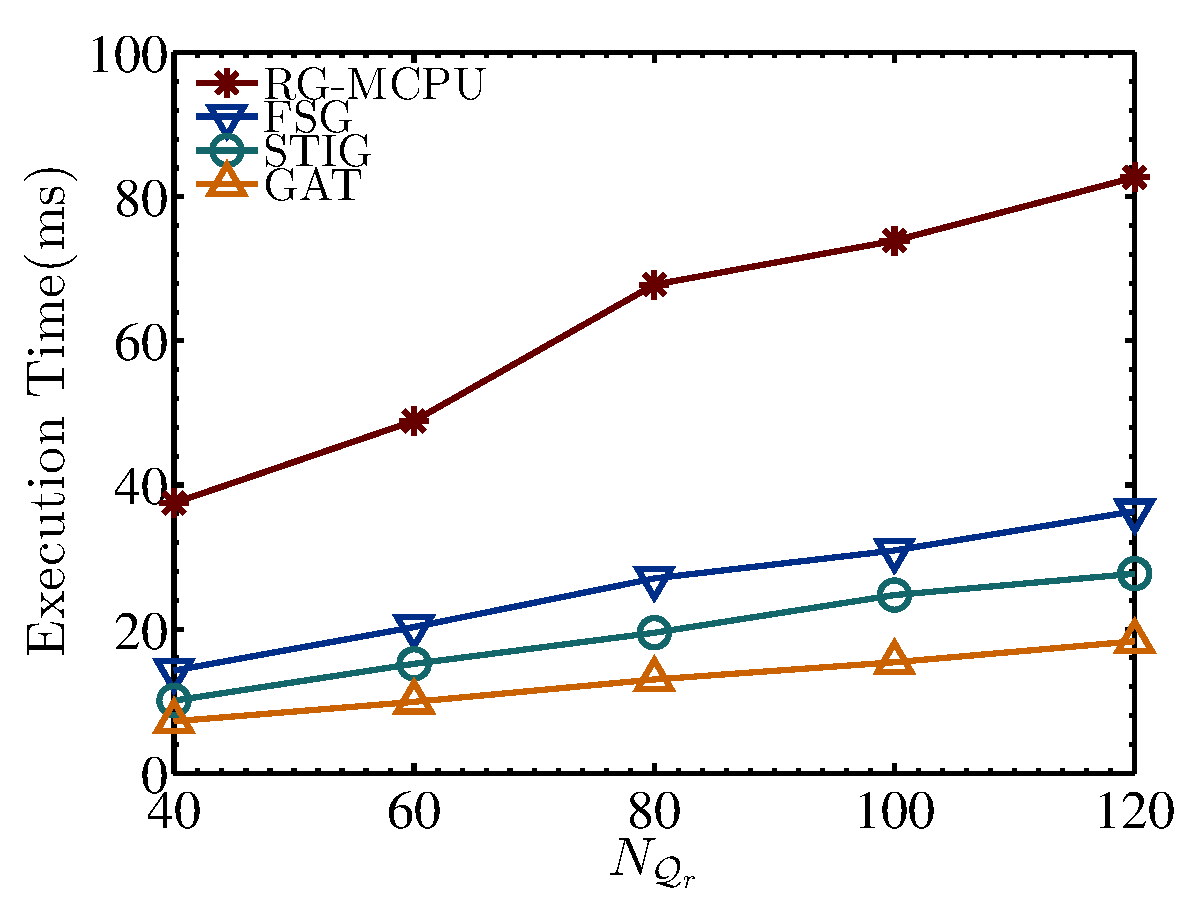
\includegraphics[width=\linewidth]{eps/QueryNum_RangeQ_GEO.eps}
			(a) Execution time for different number of range queries 
		\end{minipage}
		\hfill
		\begin{minipage}{0.48\linewidth}
			\centering
			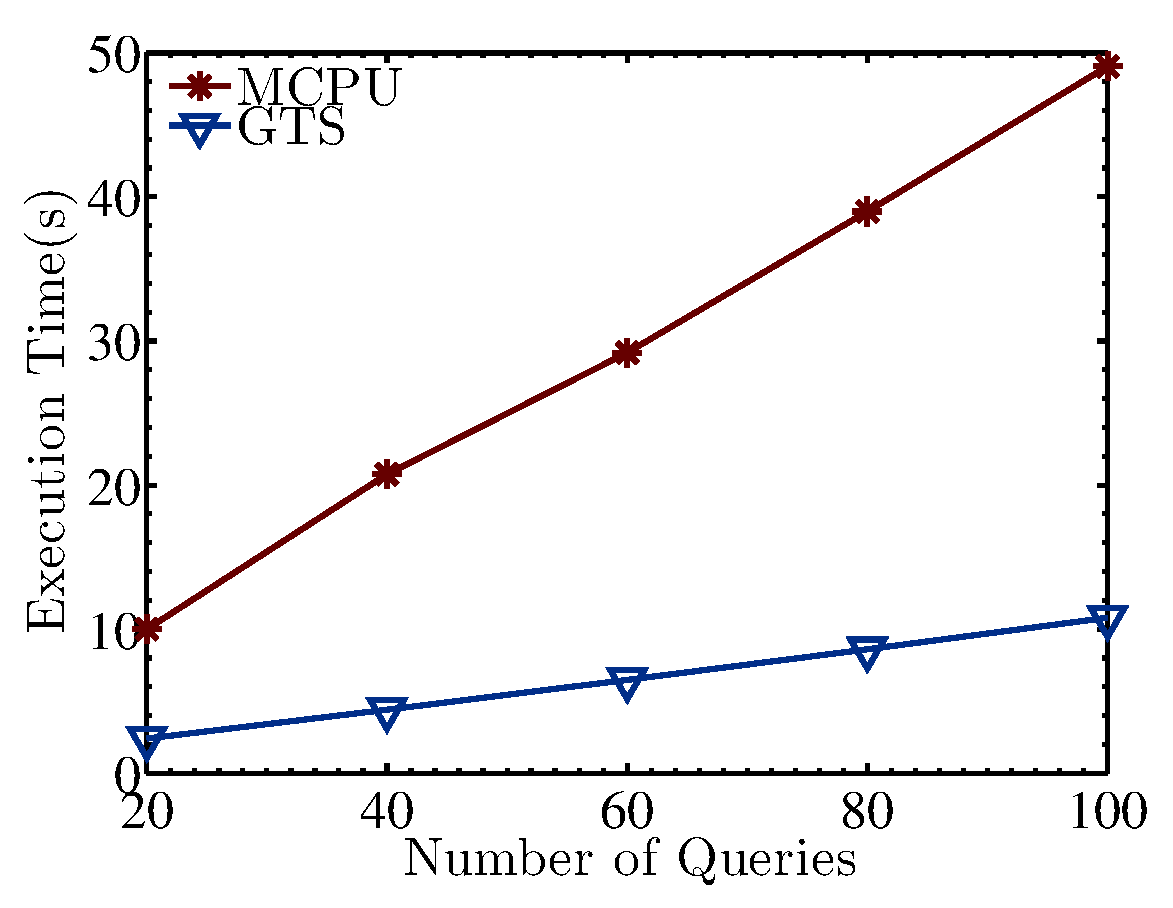
\includegraphics[width=\linewidth]{eps/QueryNum_SimilarityQ_GEO.eps}
			(b) Execution time for different number of top-k similarity queries
		\end{minipage}
	}
	\caption{Query performance for range query and top-k similarity query under different workload\label{fig:QueryNum_GEO}}
\end{figure}

\noindent \textbf{Range Query} We evaluate the efficiency of three baselines and our system under different workloads. The workload is controlled by the number of range queries with the same MBR. The result is shown in figure\ref{fig:QueryNum}, we can see that our approach outperforms other three baselines. The reason that two GPU baseline, FSG and STIG, perform worse that MCPU is because the main cost of them is the data transfering between GPU and CPU, which is getting larger as the increasing scale of queries. In our system, owing to the memory allocation table, we can avoid duplicated data transfering on the slow PCI-E interface. On the other hand, in our approach refinement workload on GPU is even, leading to more efficient parallelism. We can also see that query execution time of our approach grows linearly with increasing number of range queries. Also hundreds of queries can be finished within 200 ms, which meet the requirement of real-time service.

\noindent \textbf{Top-k Similarity Query} We test the performance of the baseline method and our system. The number of queries are set between 10 and 70 to show the time consumption under different workload. From the result shown in figure\ref{fig:QueryNum}, we can see that GPU-based approach we proposed outperforms original method implemented on multicore-CPU under all workload, because of much higher throughtput of GPU. Moreover, as the increasing number of queries, the gap between these two methods becomes larger. This is because our method mainly accelerate the calculation of EDR distance, and the propotion of time consumed in this part under high workload is much larger than that under low workload. Note that the time taken to finish top-5 similarity query for 70 trajectories having 1024 points in our GPU-based implementation is only about 38s, which is drastically shorter than that of implementation on multicore-CPU.

%\begin{figure}[!t]\centering
%	\includegraphics[width=8cm]{pdf/SpeedUp.pdf}
%	\caption{Speedup ratio of both range query and top-k similarity query on one GPU and two GPUs respectively, compared to the single-core CPU implementation\label{fig:SpeedUp}}
%\end{figure}





\subsection{Indexing Cost}

\begin{figure}[!t]\centering
	\scriptsize{
		\begin{minipage}{0.48\linewidth}
			\centering
			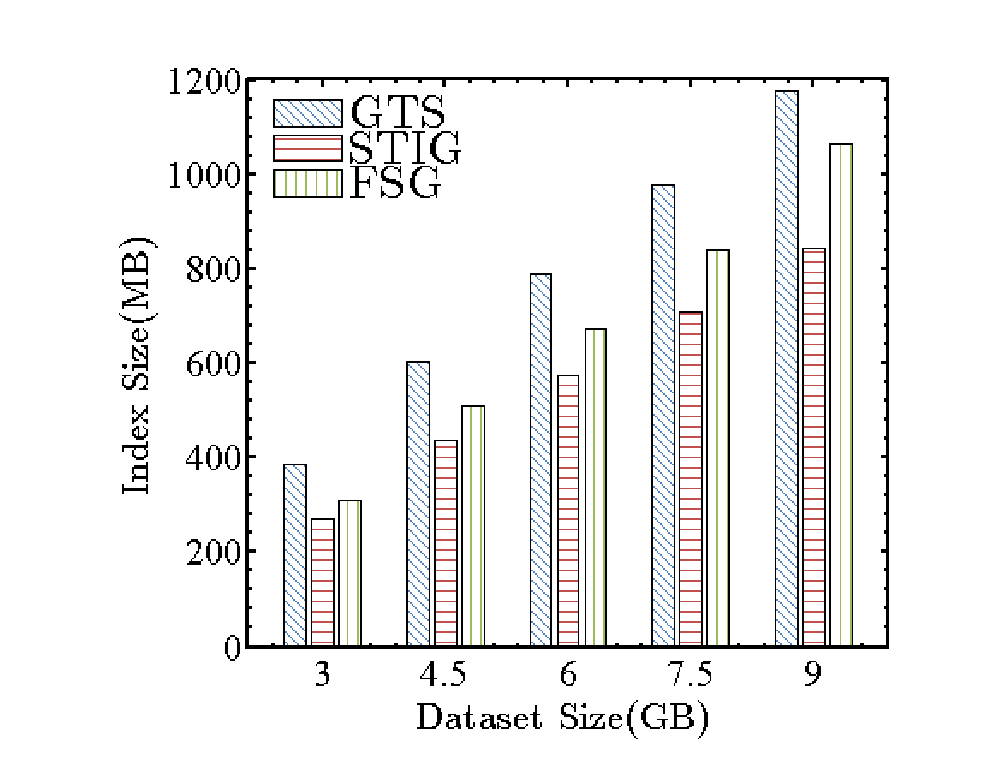
\includegraphics[width=\linewidth]{eps/indexSize.eps}
			(a) The memory occupation of index on different size of dataset
		\end{minipage}
		\hfill
		\begin{minipage}{0.48\linewidth}
			\centering
			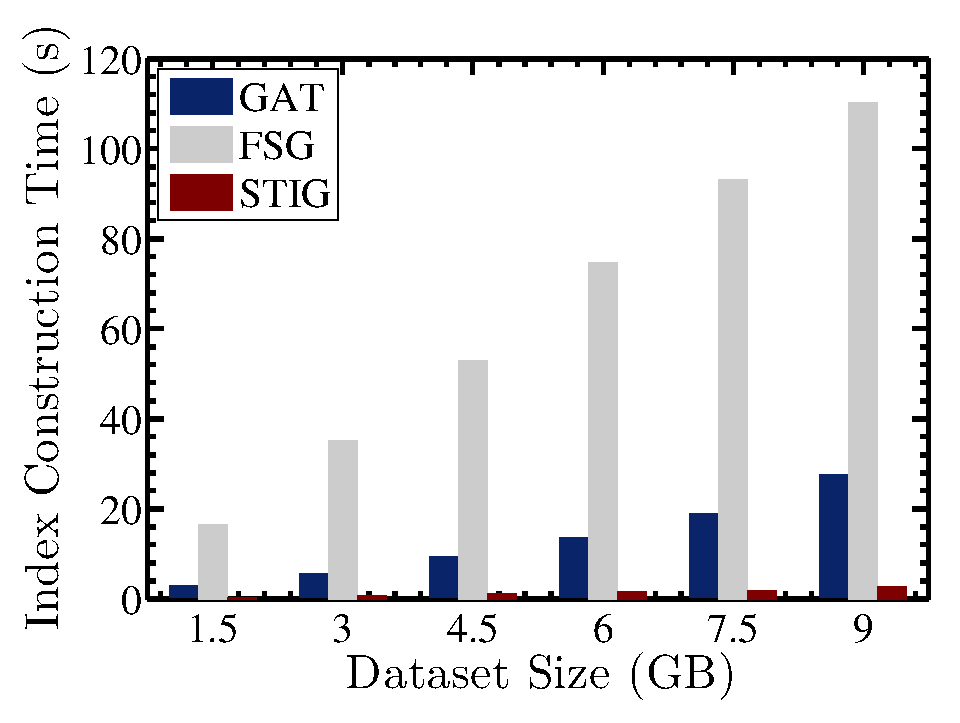
\includegraphics[width=\linewidth]{eps/indexTime.eps}
			(b) The index building time of index on different size of dataset
		\end{minipage}
	}
	\caption{The memory occupation and building time of index under different size of dataset\label{fig:IndexCost}}
\end{figure}

We then test the indexing cost of our system. We measure the memory occupation and building time of different indices in the baselines and show it in figure \ref{fig:IndexCost}. All the parameters are set to default. We can see in the evaluation of 9GB dataset our approach only use about 80MB more memory to support efficient top-k similarity query. This is because some information such as fixed grid and cell-based trajectories can be reused in both range query and top-k similarity query, so only a quadtree causes the extra occupation of memory. We argue that it is worthy to pay this small cost as a unified index for both two kinds of queries because in the most of applications we concern more about speed of query processing than a little more memory occupation. From figure \ref{fig:IndexCost}, we can see our approach spends less time in building index than STIG, because in STIG there is a large amount of computation of finding medium value when generating a layer of kd-tree.

\subsection{Speedup Ratio}
In this section we study the speedup attained by our GPU-based approach under default parameters with one and two GPUs are used. Note that 2496 CUDA cores whose frequency is 562MHz are avaliable in each GPU. We compute the speedup against the implementation on a single-core CPU whose frequency is 2.3GHz. This study explains two benefits. First, it shows that our GPU-based implementation can outperform traditional implementation on CPU. Second, it demonstrates that a near-linear improvement of efficiency can be achieved by adding more GPU devices.

\begin{table}[!h]
	\centering
	
	\caption{Speedup achieved in two datasets}     % NOTE!  caption goes _before_ the table contents !!
	\label{tab:speedup}
	
	\begin{small}
		\begin{tabular}{|l|c|c|c|c|}
			\hline
			{\bfseries Dataset} & \multicolumn{2} {c|} {\bfseries SHCAR} & \multicolumn{2} {c|} {\bfseries GeoLife} \\
			\cline{1-5}
			{\bfseries \# GPU} & {\bfseries 1GPU} &  {\bfseries 2GPU}  & {\bfseries 1GPU} &  {\bfseries 2GPU}  \\
			\hline
			Range Query & 20.07 & 37.63 & 18.03 & 32.43 \\
			\hline
			Top-k Similarity Query & 35.54 & 68.53 & 38.94 & 74.95 \\
			\hline
		\end{tabular}
	\end{small} 
\end{table}

Table \ref{tab:speedup} shows the speedup ratio for two kinds of queries. Our approach achieves about 80x speedup in evaluation of top-k similarity query for single GPU, and 42x in dual GPUs environment. The high speedup ratio comes from the parallel execution of compute-intensive calculation of EDR distance. For range query, although our approach achieves about 8.28x speedup for single GPU and 14.59x speedup for dual GPUs, slow data transfering between main memory and GPU may restrict the speedup ratio. This is because only some comparison operations are needed in the refinement procedure of range query, which means it is not a compute-intensive task.

\subsection{Scalability}

We investigate the scalability of all of the approaches in this part. Figure x presents the results under different size of data in the range from 3GB to 9GB.

\begin{figure}[!t]\centering
		\scriptsize{
		\begin{minipage}{0.48\linewidth}
			\centering
			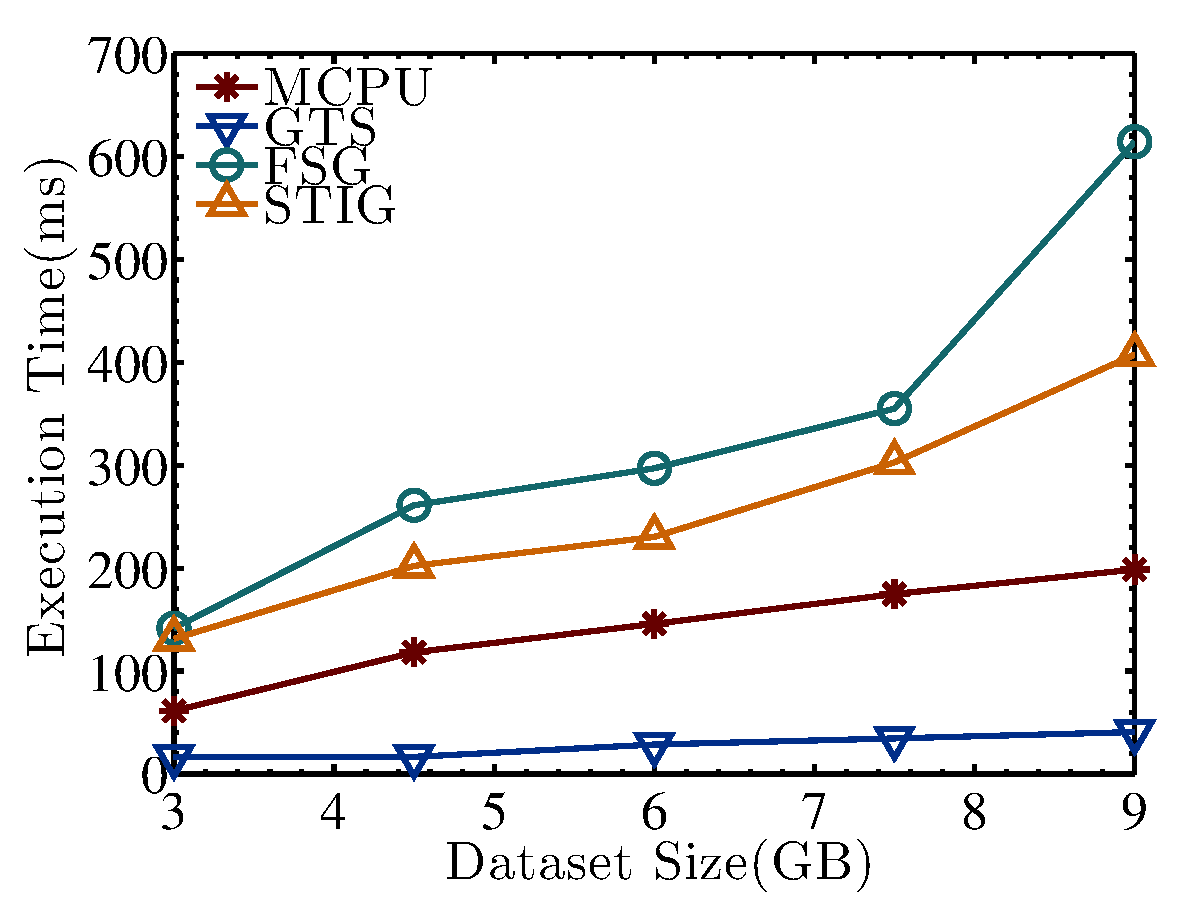
\includegraphics[width=\linewidth]{eps/range_scala.eps}
			(a) Execution time of range queries under different size of data 
		\end{minipage}
		\hfill
		\begin{minipage}{0.48\linewidth}
			\centering
			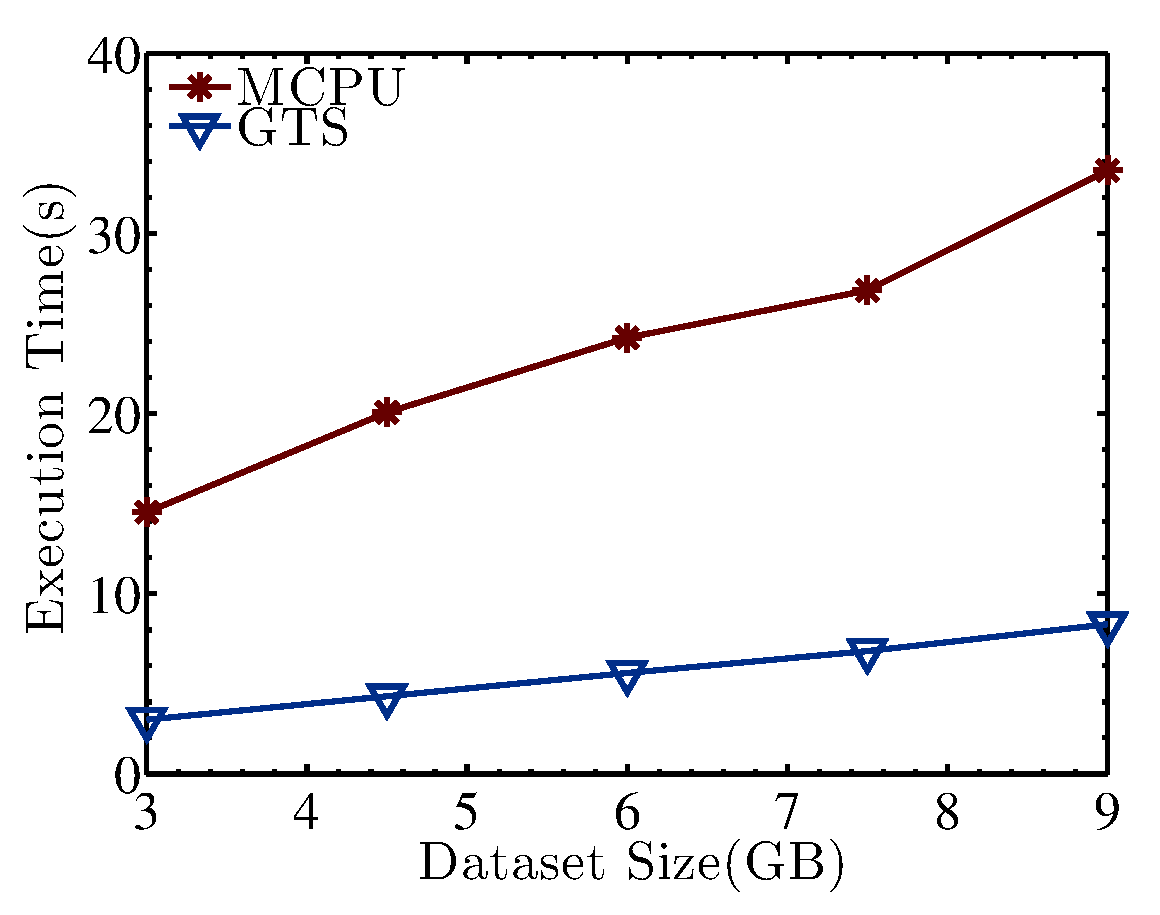
\includegraphics[width=\linewidth]{eps/similarity_scala.eps}
			(b) Execution time of top-k similarity queries under different size of data 
		\end{minipage}
	}
	\caption{Execution time of 80 range queries (left) and 40 top-k similarity queries (right) under different size of dataset\label{fig:Scalability}}
\end{figure}

\noindent \textbf{Range Query} From figure x(a) we can see that in the evaluation about range query, all the approaches increases almost linearly when we enlarge the MBR of the query. This is determined by the fact that more candidates are included in range queries if there are more points in dataset. We can also see our approach shows a better performance than other baselines in the test of each size of dataset, proving our system has a good scalability on range query.

\noindent \textbf{Top-k Similarity Query} The execution time of top-k similarity queries on different size of dataset is shown in figure \ref{fig:Scalability}. We can see as the growing volume of data, both two approaches consume more time on queries and the benefit of acceleration by using GPU becomes more obvious. It also proves that our system works excellently on large-scale dataset.


\subsection{Parameters Tuning}

In this section we study the effects of parameters in GTS. Here are totally seven parameters in our experiment as Table\ref{table_param} shows. Some of them can be categorized as query parameters, which are properties of queries and can be evaluated in both other systems and GTS, such as the area of MBR and $k$. Others are system parameters, which only exist in our system. For this reason, we show results of all baselines when evaluating the execution time in different query conditions to demonstrate both the expected performance in various environment and the effects of these parameters. Meanwhile, system parameters are evaluated under different query scales to show the effects, which are only based on our approach. 

\noindent \textbf{Range Query} There are three parameters about range query. We will evaluate the effects of them and explain the reasons.

\begin{figure}[!t]\centering
	\scriptsize{
		\begin{minipage}{0.48\linewidth}
			\centering
			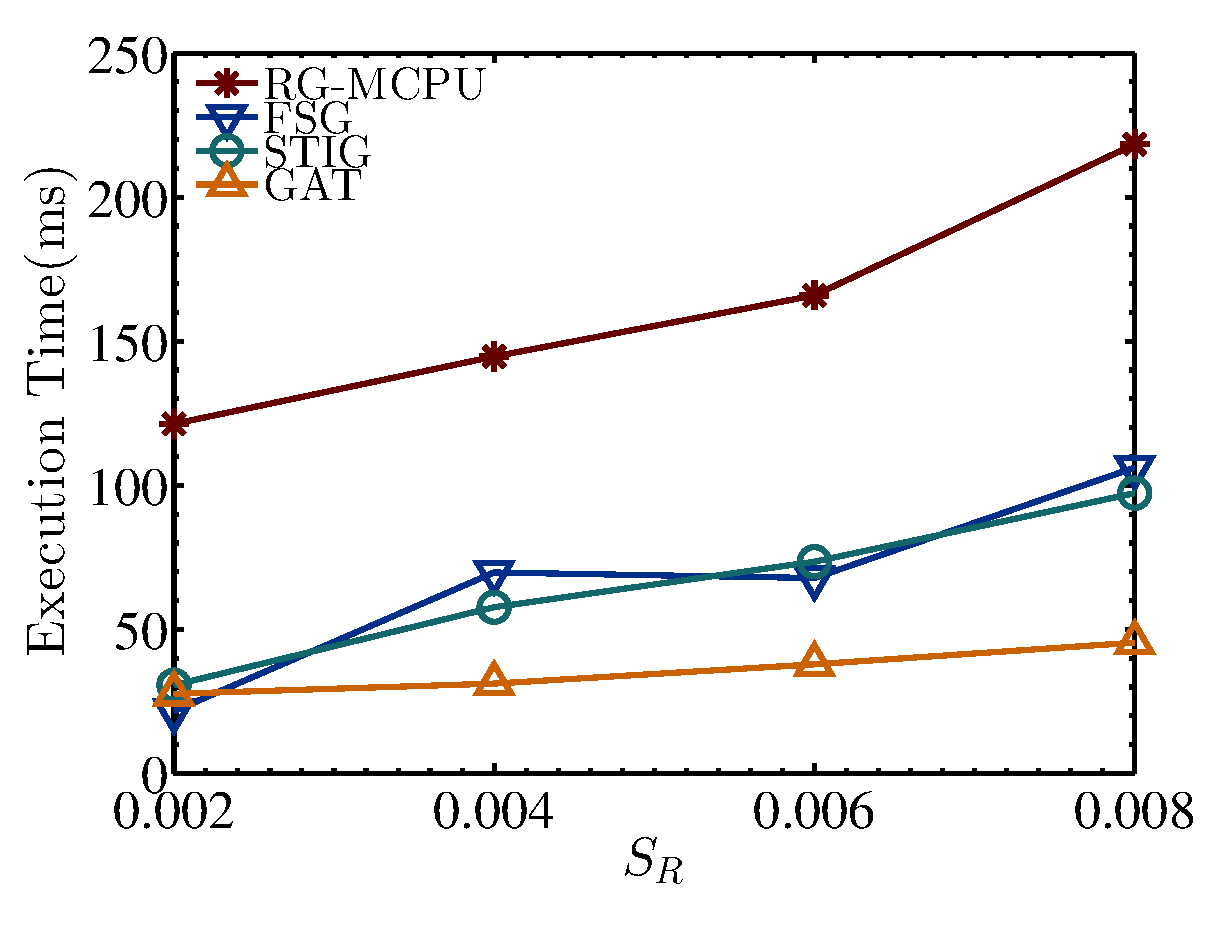
\includegraphics[width=\linewidth]{eps/RangeArea.eps}
			(a) Execution time of 80 range queries under different area of MBR
		\end{minipage}
		\hfill
		\begin{minipage}{0.48\linewidth}
			\centering
			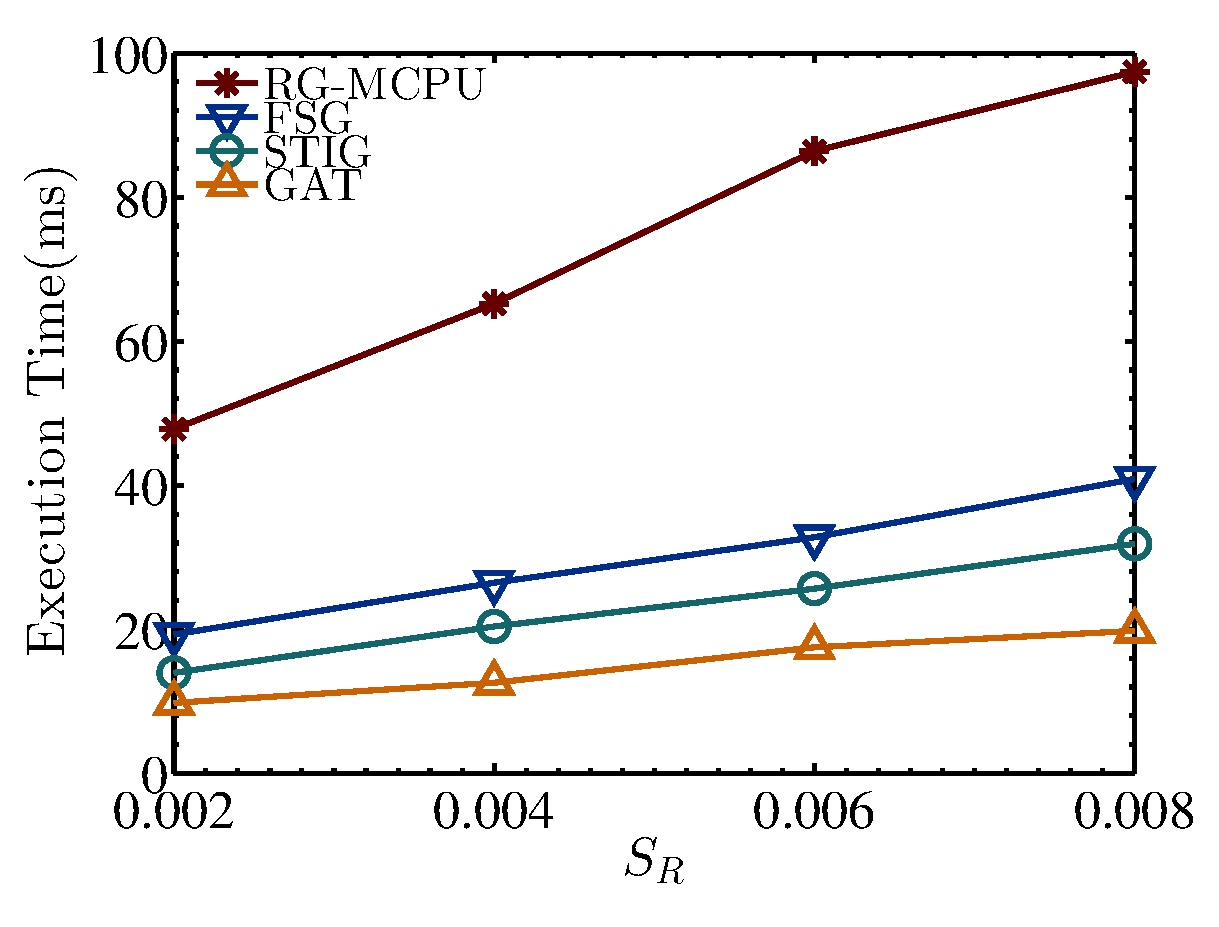
\includegraphics[width=\linewidth]{eps/RangeArea_GEO.eps}
			(b) Execution time of 80 range queries under different area of MBR
		\end{minipage}
	}
	\caption{The execution time (left) and speedup ratio achieved (right) in the top-k similarity queries \label{fig:RANGE}}
\end{figure}


$S_{RQ}$ is the only one query parameter about range query. Figure\ref{fig:RANGE} shows the time consumption of queries with different $S_{RQ}$. We can see in all approaches, the time consumption rises as the area of MBR increases from 0.002 to 0.008. We can see that this trend is nearly linear, because the number of nodes overlapped by the MBR is basically propotional to the area of MBR. 

\begin{figure}[!t]\centering
	\scriptsize{
		\begin{minipage}{0.48\linewidth}
			\centering
			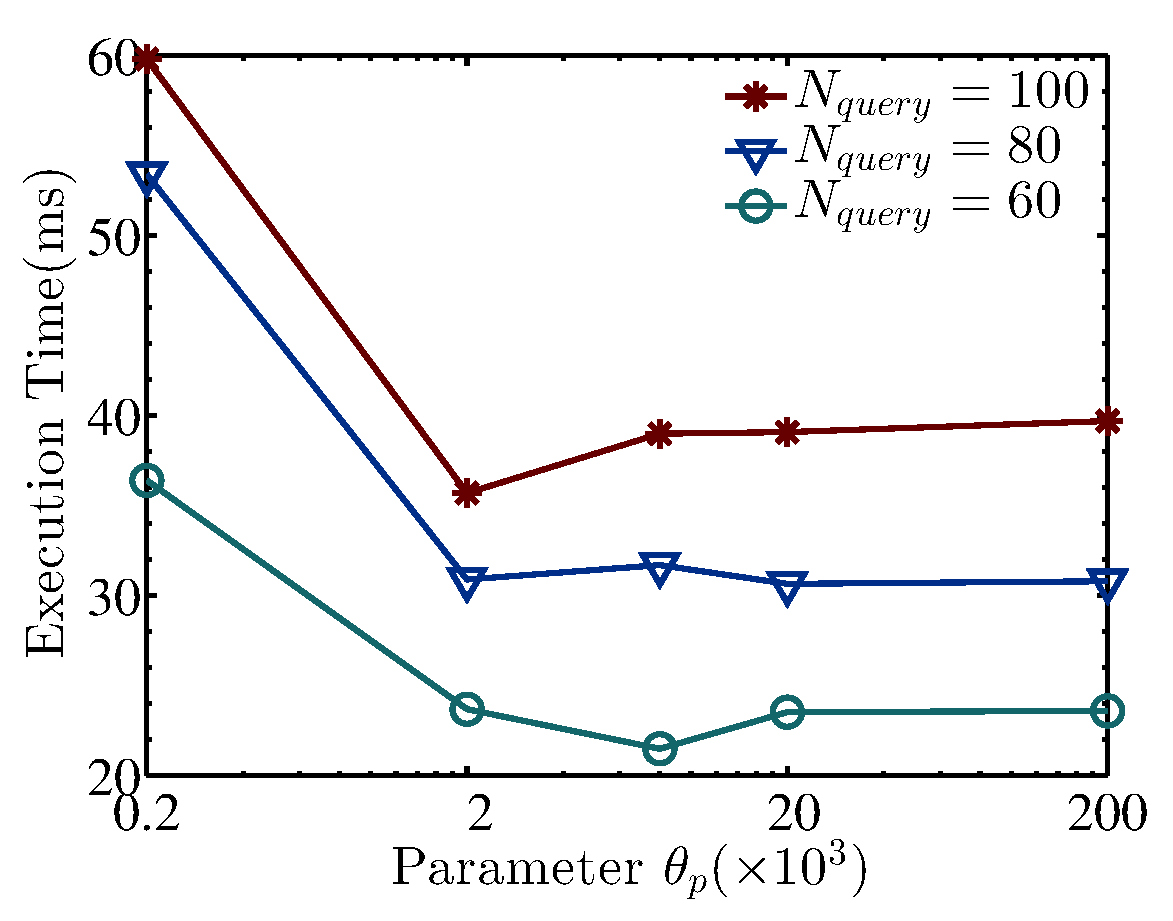
\includegraphics[width=\linewidth]{eps/MCELL.eps}
			(a) Execution time of 80 range queries under different $M_{cell}$
		\end{minipage}
		\hfill
		\begin{minipage}{0.48\linewidth}
			\centering
			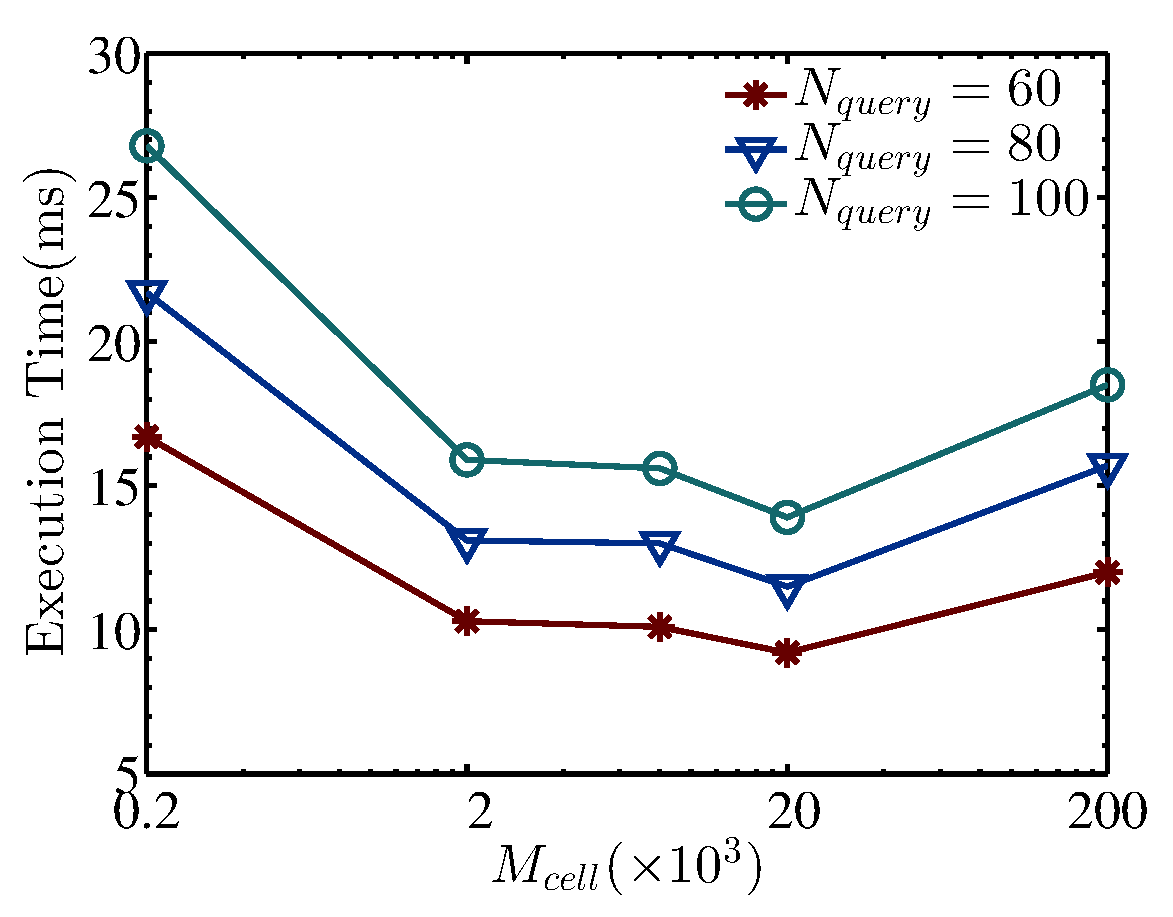
\includegraphics[width=\linewidth]{eps/MCELL_GEO.eps}
			(b) Execution time of 80 range queries under different $M_{cell}$
		\end{minipage}
	}
	\caption{The execution time (left) and speedup ratio achieved (right) in the top-k similarity queries \label{fig:MCELL_GEO}}
\end{figure}

There are two system parameters about range query: $L_{cell}$ and $M_{cell}$. As shown in figure \ref{fig:MCELL}, under $M_{cell}=2000$ and $M_{cell}=20000$ our approach achieves the best performance in all tests. We can see a downward trend of execution time as decreasing $M_{cell}$. This is because if $M_{cell}$ is too small, each SM of GPU need only finish several tests of whether a point is in MBR, leading to not fully usage of GPU. As a consequence, time consumption other than refinement itself such as memory allocation, data copy and kernel launching becomes the main source of cost. However, as $M_{cell}$ continues to increase, the workload of some refinement tasks are larger than others, causing a slight increasing of the execution time. 

\begin{figure}[!t]\centering
	\scriptsize{
		\begin{minipage}{0.48\linewidth}
			\centering
			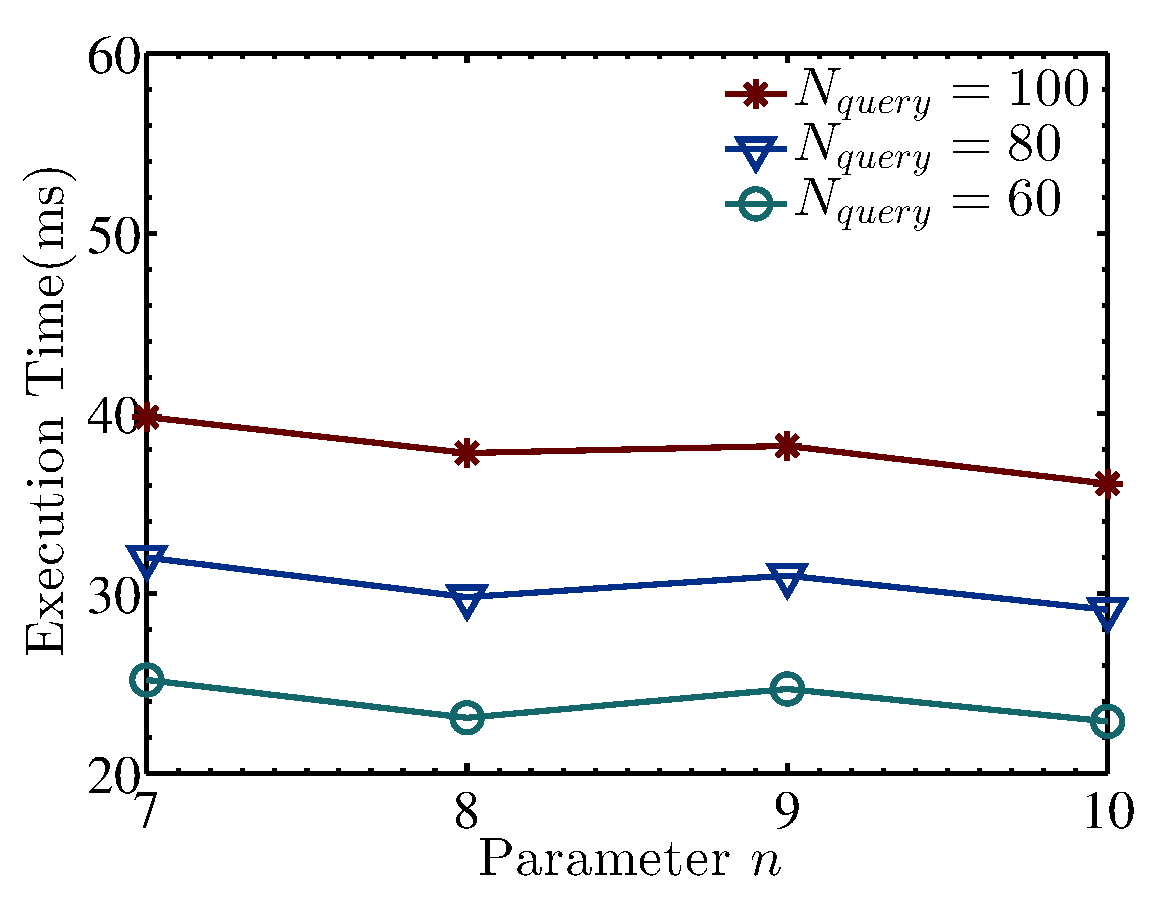
\includegraphics[width=\linewidth]{eps/LCELL.eps}
			(a) Execution time of 80 range queries under different $L_{cell}$
		\end{minipage}
		\hfill
		\begin{minipage}{0.48\linewidth}
			\centering
			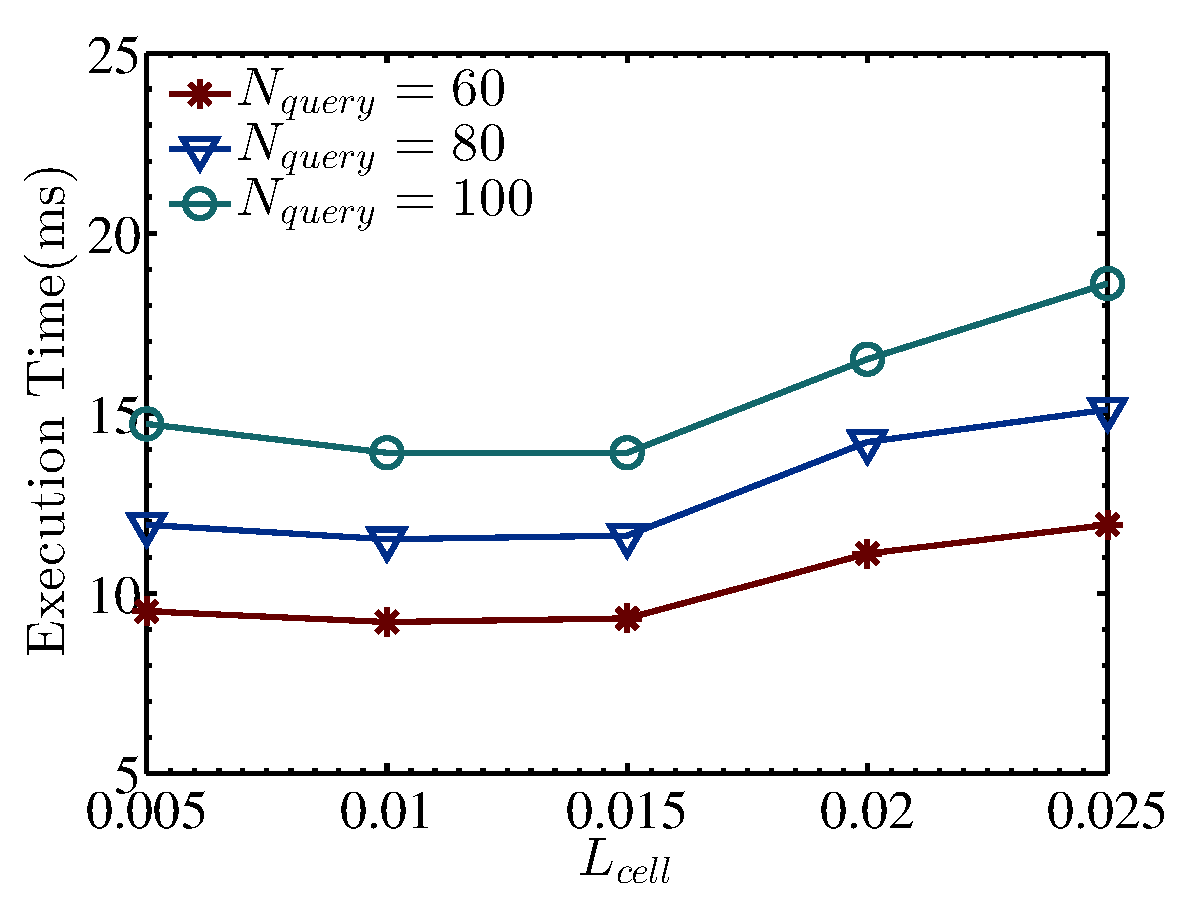
\includegraphics[width=\linewidth]{eps/LCELL_GEO.eps}
			(b) Execution time of 80 range queries under different $L_{cell}$
		\end{minipage}
	}
	\caption{The execution time (left) and speedup ratio achieved (right) in the top-k similarity queries \label{fig:LCELL}}
\end{figure}

Figure \ref{fig:LCELL} shows the running time by varying the number of $L_{cell}$ from 0.01 to 0.03. From the results, we observed that the running time tends to get larger under big $L_{cell}$. The reason is that in this situation, a larger quantity of points are collected as the candidates in filter phase. To explain it, considering an extreme situation that $L_{cell}$ is so large that there is only one cell in the whole plane.In this situation all of points are verified in refinement phase, which means that the whole process degrades to sequencial scan. However, this does not mean that smaller $L_{cell}$ is always better, because larger number of cells are generated, resulting in a slight increasing performance but much higher memory cost.

\noindent \textbf{Top-k Similarity Query} In this section, we study the effects of parameters in top-k similarity query, including $L_{query}$, $k$ and $VC$. We omit $\epsilon$ because it is considered when studying the effect of $VC$.

\begin{figure}[!t]\centering
	\scriptsize{
		\begin{minipage}{0.48\linewidth}
			\centering
			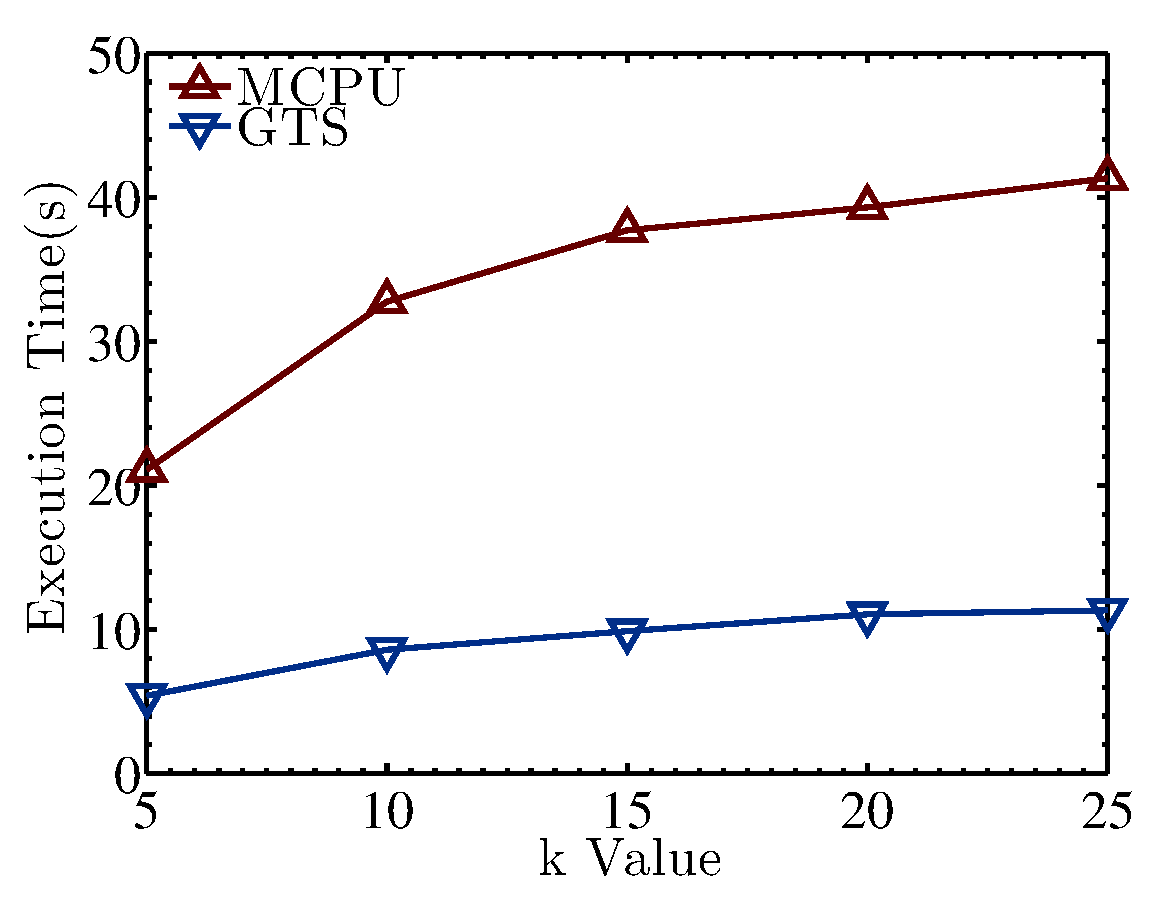
\includegraphics[width=\linewidth]{eps/kValue.eps}
			(a) Execution time of 40 top-k similarity queries with different query trajectory length
		\end{minipage}
		\hfill
		\begin{minipage}{0.48\linewidth}
			\centering
			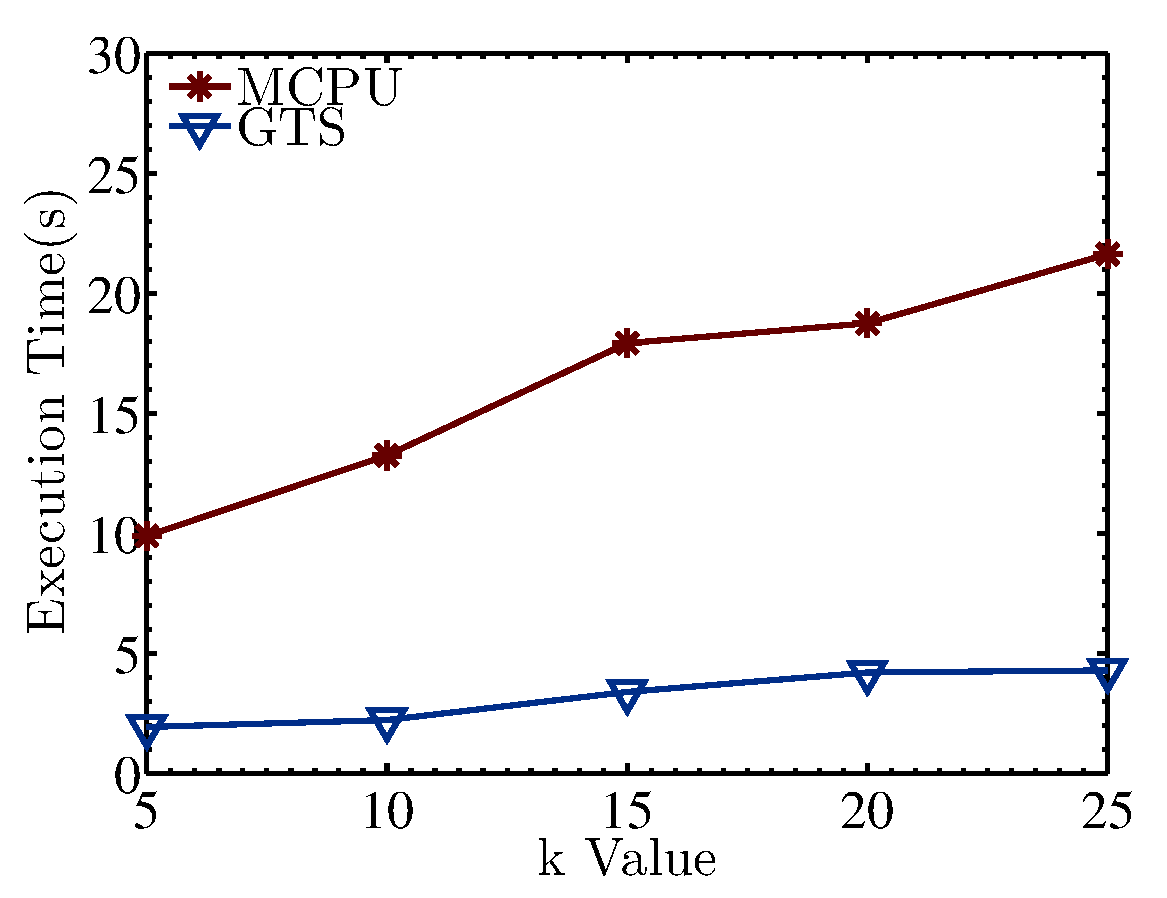
\includegraphics[width=\linewidth]{eps/kValue_GEO.eps}
			(b) Speedup ratio of 40 top-k similarity queries with different query trajectory length
		\end{minipage}
	}
	\caption{The execution time (left) and speedup ratio achieved (right) in the top-k similarity queries \label{fig:kValue}}
\end{figure}

Figure x shows the execution time of our approaches for different value of $k$. We can see that for all $k$ values our approach achieves a better performance than CPU-based implementation, and the execution time goes higher as the $k$ value increases. This is because a larger $k$ means less trajectories are filtered than that of small $k$. For example, for $k=5$, trajectories whose lowerbound of EDR are higher than the 5-th highest EDR in the priority queue will be filtered, but if $k=25$ less trajectories will be filtered because more trajectories will have a lowerbound which is lower than the highest EDR of trajectory on the tail of the priority queue. 


\begin{figure}[!t]\centering
			\scriptsize{
		\begin{minipage}{0.48\linewidth}
			\centering
			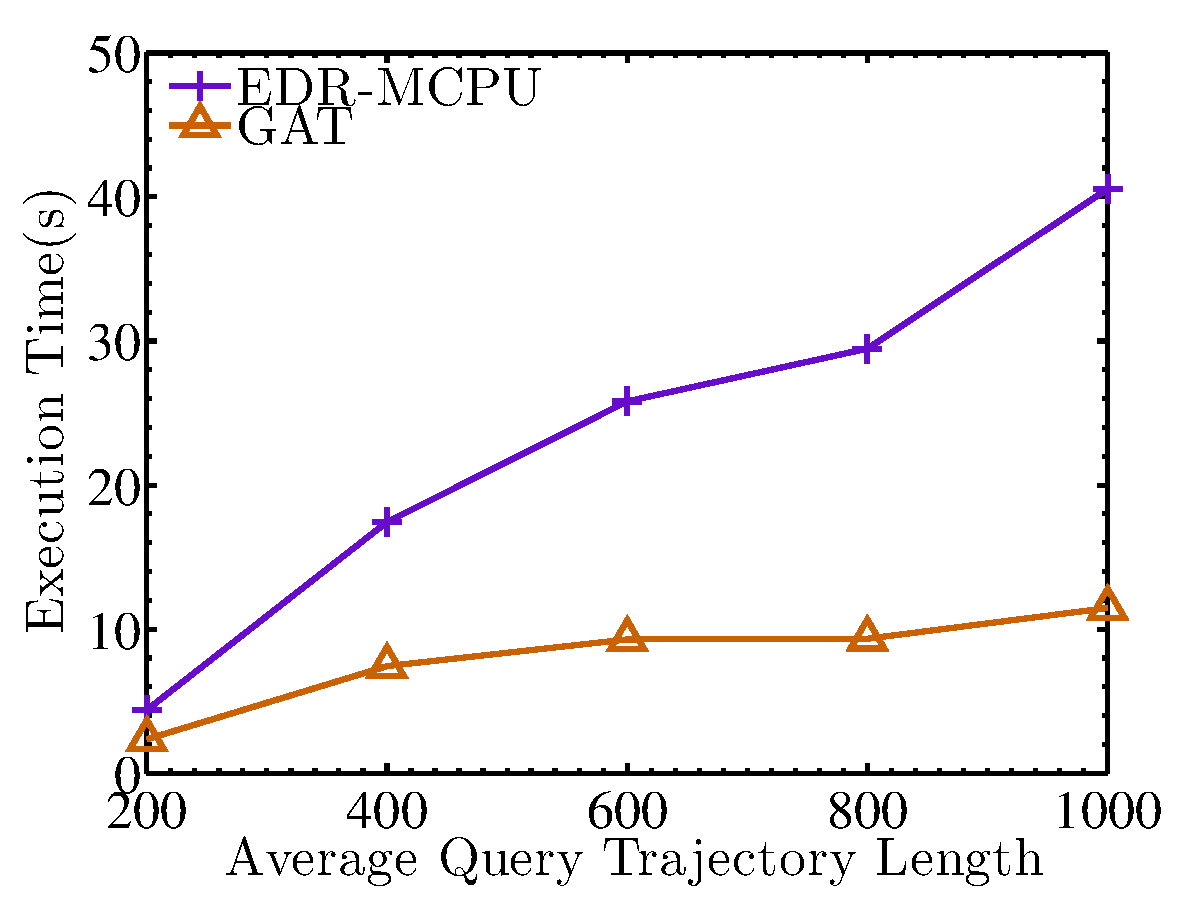
\includegraphics[width=\linewidth]{eps/QueryLength.eps}
			(a) Execution time of 40 top-k similarity queries with different query trajectory length
		\end{minipage}
		\hfill
		\begin{minipage}{0.48\linewidth}
			\centering
			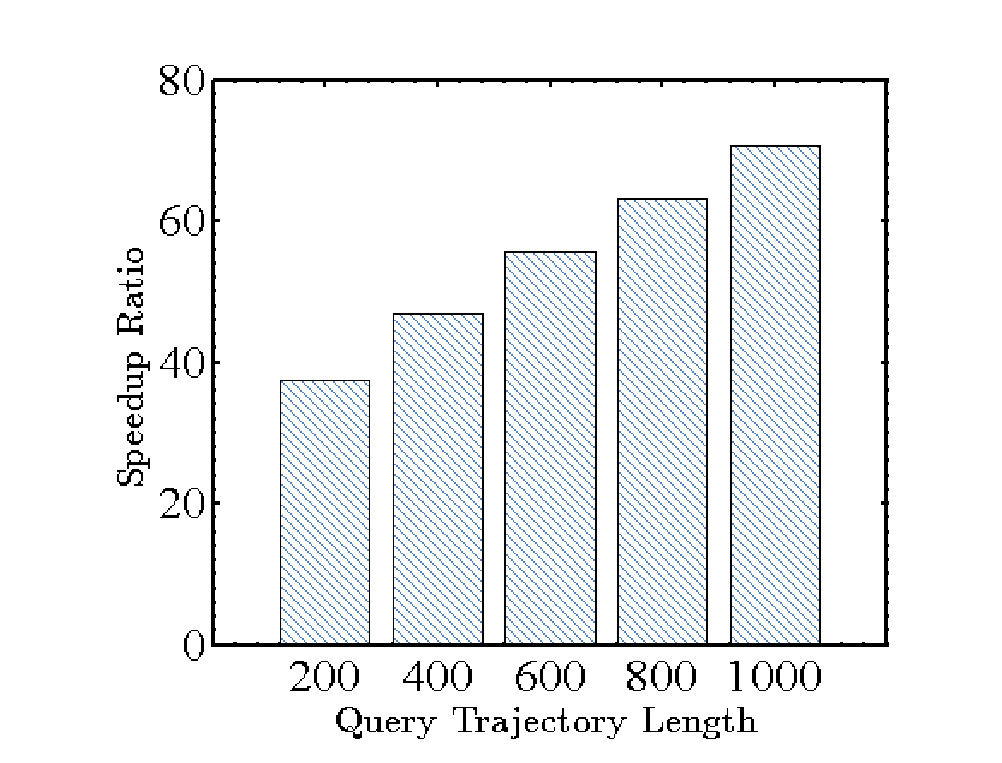
\includegraphics[width=\linewidth]{eps/QueryLength_speedup.eps}
			(b) Speedup ratio of 40 top-k similarity queries with different query trajectory length
		\end{minipage}
	}
	\caption{The execution time (left) and speedup ratio achieved (right) in the top-k similarity queries \label{fig:LENSIMI}}
\end{figure}

We then study the effects of the length of trajectories in query set. To concern on the effects of trajectories' length, we control other factors by using trajectories with the same cell-based trajectory but different length to form a query set. Figure x shows the execution time and speedup ratio for query sets which are built with trajectories of different length. It can be seen that speedup ratio rises linearly as the growing length of trajectories in query set. This phenomenon proves the cost computed in equation (x), meaning that our approach can achieve a higher speedup if trajectories in query set are longer. 

\begin{figure}[!t]\centering
	\scriptsize{
		\begin{minipage}{0.48\linewidth}
			\centering
			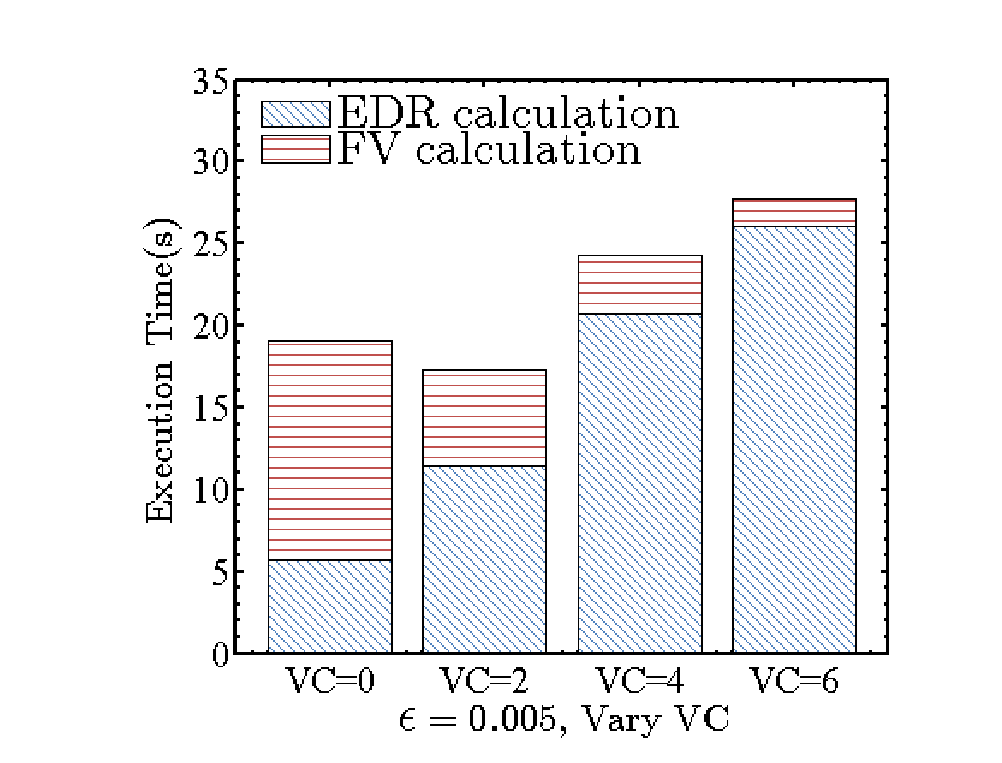
\includegraphics[width=\linewidth]{eps/VC_epsilon.eps}
			(a) Execution time of 40 top-k similarity queries with different query trajectory length
		\end{minipage}
		\hfill
		\begin{minipage}{0.48\linewidth}
			\centering
			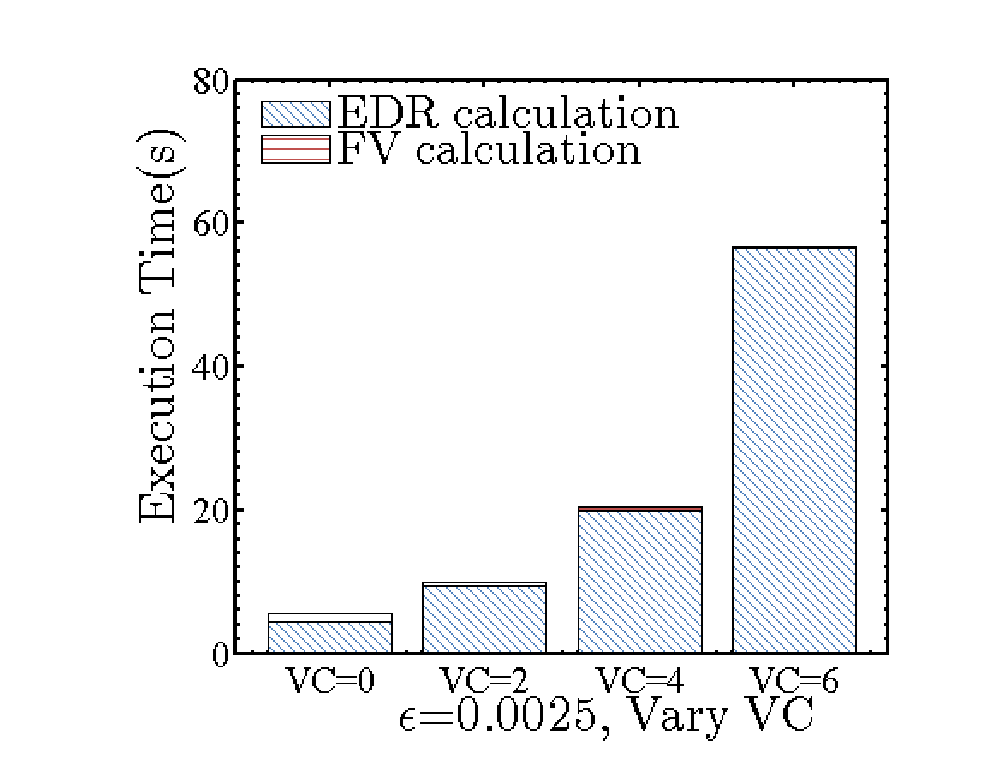
\includegraphics[width=\linewidth]{eps/VC_epsilon_GEO.eps}
			(b) Speedup ratio of 40 top-k similarity queries with different query trajectory length
		\end{minipage}
	}
	\caption{The execution time (left) and speedup ratio achieved (right) in the top-k similarity queries \label{fig:VC}}
\end{figure}

$VC$ is a system parameter which has effects on the process of pruning, as we described in section V. Because for different $\epsilon$ the most suitable $VC$ value is not the same, we study the effects of $VC$ based on the situation that $\epsilon$ equals 0.005. Figure x shows the change of pruning time and EDR calculation time under different $VC$. It can be seen that the most appropriate $VC$ is 2. When $CV$ is bigger than 2, the total execution time shows an increasing trend because of too many EDR calculation caused by the more coarse index. On the other hand, there is also high total time consumption if $CV$ is 0, and it is because more time is spent in generating FVs when the index is too fine. We can see it is important to set a correct $CV$ for acheiving a better query performance. 

\section{Related Work}\label{sec:related}

There has been various related works about trajectory storage, indexing and query processing. In this sectoin we review some previous related works about Trajectory Storage and Indexing, Spatial Query Processing.

\subsection{Trajectory Indexing and Query Processing}

R-Tree~\cite{DBLP:conf/sigmod/Guttman84} is the most classical index for spatial data, which is a two-dimensional generalization of B-Tree~\cite{DBLP:conf/sigmod/BayerM70}. However, it is not good enough for large-scale trajectory data as the large number of overlappings among the MBR. After that some indices optimized for trajectory such as 3D-RTree~\cite{DBLP:conf/icmcs/TheodoridisVS96}, TB-Tree~\cite{DBLP:conf/vldb/PfoserJT00} and TPR-Tree~\cite{DBLP:conf/sigmod/SaltenisJLL00}. They index on the temporal dimension as well as the spatial dimension. However, they are non-adaptive, meaning that they suffered from a performance loss as the diversity of trajectory distribution. SETI~\cite{DBLP:conf/cidr/ChakkaEP03} proposed a indexing mechanism which forms a two-level index by decoupling the spatial dimension and temporal dimension to reduce the complexity of spatial query. PIST~\cite{DBLP:journals/geoinformatica/BoteaMNS08} developed a cost model of partitioning the data space for different data distributions, aiming to reduce the number of disk accesses. TrajStore~\cite{DBLP:conf/icde/Cudre-MaurouxWM10} proposed an adaptive algorithm to split trajectories optimally and cluster them physically to achieve a lowest expected cost of query according to the model about the number of pages accessed when executing range queries. Different to the above works which are based on the optimization to the I/O cost, Wang et.al. developed an in-memory column-oriented storage called SharkDB~\cite{DBLP:conf/cikm/WangZXZZS14} to achieve the high performance in range queries and kNN queries by avoiding the expensive I/O operations. Trajtree~\cite{EDWP15} was designed to index the computation of EDwP, a similarity metric optimized for trajectories under inconsistent sampling rates. However, these works are all designed to process queries on single-core CPU, so the performance in big trajectory data environment is limited.

There are also some previous works which accelerate various queries on trajectory data using GPU. Zhang et.al~\cite{Zhang:2012:USH} proposed a prototype system called U$_2$STRA to achieve high performance in querying of large-scale trajectory data. It used a four-level hierarchy to split and represent trajectories, and then index them by a grid-file based data structure. Based on this system, he developed TKSimGPU~\cite{DBLP:conf/bigdataconf/LealGZY15}, a top-k similarity query algorithm for multicore CPU and manycore GPU, to fill the gap between the importance of this query and the lack of parallel algorithm for it. However, it only support a similarity metric called Hausdorff distance, which is not as popular and robust as some metrics based on global alignment such as EDR~\cite{DBLP:conf/sigmod/ChenOO05}, DTW~\cite{DBLP:conf/vldb/Keogh02} and EDwP~\cite{EDWP15}. Gowanlock et.al~\cite{DBLP:journals/tpds/GowanlockC16} developed three GPU-friendly indexing schemes for distance threshold similarity searches for trajectories, in which the segments within an euclidean distance threshold in a point of time are retrieved. Its aims are different from our work, in which all points of time is considered in similarity searches.

\subsection{Parallel and Distributed Spatial Data Analytics}

Apart from trajectory, some parallel spatial data analytics frameworks and systems are proposed for spatio-temporal data before. Zhang et.al~\cite{GPUTaxi} developed a query processing system to manage big taxi trip data, which record the pickup locations and timestamps of the passengers, by the help of GPU. Lettich et.al~\cite{DBLP:conf/gis/LettichOS15} designed the PR-quadtree to process stream spatial k-NN queries, in which GPU is used to constructing the index within one second and executing a mass of queries in following seconds to meet the requirement of short response time. Doraiswamy et.al.~\cite{7498315} generalized the kd-tree to STIG, in which points in leaf node are packed to a block to guarantee the fully utilization of GPU when performing interative spatio-temporal queries on it. However, these works are not suitable for managing large-scale trajectory data, because trajectory is not the set but the sequence of spatio-temporal points. 

Some works utilize distributed system to solve the efficiency problem in processing spatial queries on single CPU. HadoopGIS ~\cite{DBLP:journals/pvldb/AjiWVLL0S13} adapted and extended Hadoop to meet the challenge of large-scale spatial objects and high computation complexity. It is intergrated with Hive and provides an expressive spatial query language. Lu et.al~\cite{DBLP:journals/pvldb/LuSCO12} proposed a solution to the problem of implementing kNN join, an expensive spatial operation for large dataset, in MapReduce to improve the performance of it. Aiming to the performance degradation due to the moving hotspots in distributed spatio-temporal storage system, Pyro~\cite{DBLP:conf/usenix/LiHGSA15} adapted HDFS and H-Base by employing a novel DFS block grouping algorithm and multi-scan optimization to reduce the response time of geometry queries. Based on Spark, Dong et.al developed Simba ~\cite{DBLP:conf/sigmod/XieL0LZG16} to provide native support for spatial queries to achieve low query latency and high throughput and excellent scalability. After that, he proposed a distributed framework~\cite{DBLP:journals/pvldb/XieLP17} implemented on Spark which leverage it to answer similarity searches with Hausdorff and Frechet distance as the metric. ???


\section{Conclusion}\label{sec:conclusion}
The conclusion goes here.



% conference papers do not normally have an appendix


% use section* for acknowledgement
\section*{Acknowledgment}


The authors would like to thank...


%
%
%
%\subsection{This Sub-Section for LaTeX Users Only}
%
%If the appearance is different from what is shown in this template,
%then the cause may be the use of conflicting style files in your
%LaTeX document.  An example of an incompatible style file is {\it
%latex8.sty}.  You must remove all such conflicting style files.
%
%\section{Page Layout}
%
%An easy way to comply with the conference paper formatting
%requirements is to use this document as a template and simply type
%your text into it.
%
%\subsection{Page Layout}
%
%Your paper must use a page size corresponding to US Letter which is
%215.9mm (8.5") wide and 279.4mm (11") long.  The margins must be
%set as follows:
%
%\begin{itemize}
%\item	Top = 19mm (0.75")
%\item	Bottom = 25.4mm (1")
%\item	Left = Right = 17.3mm (0.68")
%\end{itemize}
%
%Your paper must be in two column format with a space of 4.22mm
%(0.17") between columns. 
%
%\section{Page Style}
%\label{sec:page style}
%
%All paragraphs must be indented.  All paragraphs must be
%justified, i.e. both left-justified and right-justified. 
%
%\subsection{Text Font of Entire Document}
%
%The entire document should be in Times New Roman or Times font.
%Type 3 fonts must not be used.  Other font types may be used if
%needed for special purposes.  
%
%Recommended font sizes are shown in Table \ref{tab:font-sizes}.
%
%\subsection{Title and Author Details}
%\label{sec:title and author details}
%
%Title must be in 24 pt Regular font.  Author name must be in 11
%pt Regular font.  Author affiliation must be in 10 pt Italic.
%Email address must be in 9 pt Courier Regular font.  
%
%\begin{table}[!h]
%\centering
%
%    \caption{Font Sizes for Papers}     % NOTE!  caption goes _before_ the table contents !!
%    \label{tab:font-sizes}
%
%    \begin{small}
%    \begin{tabular}{|l|l|l|l|}
%    \hline
%    {\bfseries Font} & \multicolumn{3} {c|} {\bfseries Appearance (in Times New Roman or Times} \\
%    \cline{2-4}
%    {\bfseries Size} & {\bfseries  Regular}         & {\bfseries Bold}     & {\bfseries Italic}           \\
%    \hline
%    8         & table caption (in	&		& reference item	\\
%              & Small Caps),		&		& (partial)		\\
%              &	figure caption,		&		&			\\
%              &	reference item		&		&			\\
%    \hline
%    9         & author email address	& abstract body & abstract heading	\\
%              &	 (in Courier),		&		&    (also in Bold)	\\
%              &	cell in a table		&		&			\\
%    \hline
%    10        & level-1 heading  (in 	&		& level-2 heading,      \\
%              & Small Caps),		&		& level-3 heading,	\\
%              &	paragraph		&		& author affiliation	\\
%    \hline
%    11        &	author name		&		&			\\
%    \hline
%    24        & title			&		&			\\
%    \hline
%    \end{tabular}
%    \end{small} 
%\end{table}
%
%All title and author details must be in single-column format and
%must be centered. 
%
%Every word in a title must be capitalized except for short minor
%words such as ``a'', ``an'', ``and'', ``as'', ``at'', ``by'', ``for'', ``from'',
%``if'', ``in'', ``into'', ``on'', ``or'', ``of'', ``the'', ``to'', ``with''.  
%
%Author details must not show any professional title (e.g.
%Managing Director), any academic title (e.g. Dr.) or any
%membership of any professional organization (e.g. Senior
%Member IEEE).
%
%To avoid confusion, the family name must be written as the
%last part of each author name (e.g. John A.K. Smith).
%
%Each affiliation must include, at the very least, the name of
%the company and the name of the country where the author is
%based (e.g. Causal Productions Pty Ltd, Australia).  
%
%Email address is compulsory for the corresponding author.
%
%
%\subsection{Section Headings}
%
%No more than 3 levels of headings should be used.  All headings must
%be in 10pt font.  Every word in a heading must be capitalized except
%for short minor words as listed in Section \ref{sec:title and author
%details}.
%
%\subsubsection{Level-1 Heading}
%
%A level-1 heading must be in Small Caps, centered and numbered using
%uppercase Roman numerals.  For example, see heading ``\ref{sec:page
%style}. Page Style'' of this document.  The two level-1 headings which
%must not be numbered are ``Acknowledgment'' and ``References''.
%
%\subsubsection{Level-2 Heading}
%
%A level-2 heading must be in Italic, left-justified and numbered using
%an uppercase alphabetic letter followed by a period.  For example, see
%heading ``C. Section Headings'' above.
%
%\subsubsection{Level-3 Heading}
%
%A level-3 heading must be indented, in Italic and numbered with an
%Arabic numeral followed by a right parenthesis. The level-3 heading
%must end with a colon.  The body of the level-3 section immediately
%follows the level-3 heading in the same paragraph.  For example, this
%paragraph begins with a level-3 heading.
%
%\subsection{Figures and Tables}
%
%Figures and tables must be centered in the column.  Large figures and
%tables may span across both columns.  Any table or figure that takes
%up more than 1 column width must be positioned either at the top or at
%the bottom of the page.
%
%Graphics may be full color.  All colors will be retained on the CDROM.
%Graphics must not use stipple fill patterns because they may not be
%reproduced properly.  Please use only SOLID FILL colors which contrast
%well both on screen and on a black-and-white hardcopy, as shown in
%Fig.  \ref{fig:sample_graph}.
%
%\begin{figure}[h]
%	\centerline{\psfig{figure=fig_1.eps,width=68.7mm} }
%	\caption{A sample line graph using colors which contrast well both on screen and on a black-and-white hardcopy}
%	\label{fig:sample_graph}
%\end{figure}
%
%Fig. \ref{fig:lores-photo} shows an example of a low-resolution image
%which would not be acceptable, whereas Fig.  \ref{fig:hires-photo}
%shows an example of an image with adequate resolution.  Check that the
%resolution is adequate to reveal the important detail in the figure.
%
%Please check all figures in your paper both on screen and on a
%black-and-white hardcopy.  When you check your paper on a
%black-and-white hardcopy, please ensure that:
%
%\begin{itemize}
%\item	the colors used in each figure contrast well,
%\item	the image used in each figure is clear,
%\item	all text labels in each figure are legible.
%\end{itemize}
%
%\begin{figure}[h]
%	\centerline{\psfig{figure=lores_photo.eps,height=64.54mm} }
%	\caption{Example of an unacceptable low-resolution image}
%	\label{fig:lores-photo}
%\end{figure}
%
%\begin{figure}[h]
%	\centerline{\psfig{figure=hires_photo.eps,height=64.54mm} }
%	\caption{Example of an image with acceptable resolution}
%	\label{fig:hires-photo}
%\end{figure}
%
%\subsection{Figure Captions}
%
%Figures must be numbered using Arabic numerals.  Figure captions must
%be in 8 pt Regular font.  Captions of a single line (e.g. Fig.
%\ref{fig:lores-photo}) must be centered whereas multi-line captions
%must be justified (e.g. Fig.  \ref{fig:sample_graph}).  Captions with
%figure numbers must be placed after their associated figures, as shown
%in Fig. \ref{fig:sample_graph}.
%
%\subsection{Table Captions}
%
%Tables must be numbered using uppercase Roman numerals.  Table
%captions must be centred and in 8 pt Regular font with Small Caps.
%Every word in a table caption must be capitalized except for short
%minor words as listed in Section \ref{sec:title and author details}.
%Captions with table numbers must be placed before their associated
%tables, as shown in Table \ref{tab:font-sizes}.
%
%\subsection{Page Numbers, Headers and Footers}
%
%Page numbers, headers and footers must not be used.
%
%\subsection{Links and Bookmarks}
%
%All hypertext links and section bookmarks will be removed from
%papers during the processing of papers for publication.  If you
%need to refer to an Internet email address or URL in your paper,
%you must type out the address or URL fully in Regular font.
%
%\subsection{References}
%
%The heading of the References section must not be numbered.
%All reference items must be in 8 pt font.  Please
%use Regular and Italic styles to distinguish different fields as
%shown in the References section. Number the reference items
%consecutively in square brackets (e.g. ~\cite{IEEEexample:book}).
%
%When referring to a reference item, please simply use the
%reference number, as in ~\cite{IEEEexample:bookwithseriesvolume}.
%Do not use �Ref. ~\cite{IEEEexample:article_typical}� or
%�Reference ~\cite{IEEEexample:article_typical}� except at the
%beginning of a sentence, e.g.  ``Reference
%~\cite{IEEEexample:article_typical} shows �''.  Multiple
%references are each numbered with separate brackets (e.g.
%~\cite{IEEEexample:bookwithseriesvolume},
%~\cite{IEEEexample:article_typical},
%~\cite{IEEEexample:confwithpaper}--[6]).
%
%Examples of reference items of different categories shown in the
%References section include:
%
%\begin{itemize}
%\item	example of a book in ~\cite{IEEEexample:book}
%\item	example of a book in a series in ~\cite{IEEEexample:bookwithseriesvolume}
%\item	example of a journal article in ~\cite{IEEEexample:article_typical}
%\item	example of a conference paper in ~\cite{IEEEexample:confwithpaper}
%\item	example of a patent in ~\cite{IEEEexample:uspat}
%\item	example of a website in ~\cite{IEEEexample:IEEEwebsite}
%\item	example of a web page in ~\cite{IEEEexample:shellCTANpage}
%\item	example of a databook as a manual in ~\cite{IEEEexample:motmanual}
%\item	example of a datasheet in ~\cite{IEEEexample:datasheet}
%\item	example of a master's thesis in ~\cite{IEEEexample:masterstype}
%\item	example of a technical report in ~\cite{IEEEexample:techreptype}
%\item	example of a standard in ~\cite{IEEEexample:standard}
%\end{itemize}
%
%% the following command shrinks the final page to force the columns to
%% be balanced.  You will need to adjust the value according to the 
%% appearance of your last page.  Start by setting the value to 0mm
%% and slowly increase it until the columns balance.  Alternatively,
%% use balance.sty to do the job.
%\enlargethispage{-62mm}
%
%\section{Conclusion}
%
%The version of this template is V3.  Most of the formatting
%instructions in this document have been compiled by Causal Productions
%from the IEEE LaTeX style files.  Causal Productions offers both A4
%templates and US Letter templates for LaTeX and Microsoft Word.  The
%LaTeX templates depend on the official IEEEtran.cls and IEEEtran.bst
%files, whereas the Microsoft Word templates are self-contained.
%Causal Productions has used its best efforts to ensure that the
%templates have the same appearance.
%
%Causal Productions permits the distribution and revision of these
%templates on the condition that Causal Productions is credited in the
%revised template as follows: ``original version of this template was
%provided by courtesy of Causal Productions
%(www.causalproductions.com)''.
%
%\section*{Acknowledgment}
%
%The heading of the Acknowledgment section and the References section
%must not be numbered.
%
%Causal Productions wishes to acknowledge Michael Shell and other
%contributors for developing and maintaining the IEEE LaTeX style files
%which have been used in the preparation of this template.  To see the
%list of contributors, please refer to the top of file IEEETran.cls in
%the IEEE LaTeX distribution.

\bibliographystyle{IEEEtran}

\bibliography{IEEEabrv,IEEEexample}

\end{document}

